%\chapter{FITTING THE HIGH RESOLUTION SPECTRUM OF RX J0925.7-4758 USING COMPOSITE XSPEC MODEL} \label{chap:hi-resolution}
\chapter{\MakeUppercase{\ChapterTitleFour}} \label{chap:hi-resolution}
    %\doublespacing
    \minitoc
    
    \newpage
    \begin{center}
    	%\emph{Abstract of chapter \ref{chap:hi-resolution}}
    	\emph{Abstract}
    \end{center}
    This chapter presents a new analysis of high-resolution X-ray spectra of the astronomical object RX J0925.7-4758, obtained using the XMM-Newton observatory's RGS instrument. We employ spectral fitting using a model grid to ascertain the one that accurately represents the observed data. Our analysis focuses on a subset of pre-defined models, evaluating their fit quality using the reduced chi-squared statistic $\chi^2_\text{reduced}$). We find that model M11 provides the best fit ($1<\chi^2_\text{reduced}<2$) for spectra from both RGS1 and RGS2 instruments, across all observed spectral orders. This signifies a significant improvement compared to previous studies on RX J0925.7-4758, which faced challenges in modeling the object's X-ray emission using a non-local thermodynamic equilibrium (NLTE) atmosphere model. The model M11 incorporates several components, including interstellar medium (ISM) absorption, intrinsic X-ray emission with separate contributions from cold gas absorption and an NLTE atmosphere, thermal plasma emission from potentially two different mechanisms, and a wind or outflow component. This comprehensive model suggests a more accurate capture of the physical processes governing the X-ray emission from RX J0925.7-4758.
    
    \setcounter{footnote}{\value{footnotecount}}

	\newpage
	\section{\MakeUppercase{RGS Spectra from XMM-Newton}} \label{hi-resolution:rgs-spec}
		X-ray astronomy provides a powerful tool for studying the universe's most energetic phenomena. However, a complete understanding often requires detailed information about the elemental composition and physical conditions within the emitting region. This is where high-resolution X-ray spectroscopy shines, allowing us to dissect the X-ray emission line by line.
		
		The Reflection Grating Spectrometers (RGS) onboard the XMM-Newton satellite offer exceptional capabilities in this domain\footnote{\url{https://www.cosmos.esa.int/web/xmm-newton/technical-details-rgs}}. These instruments achieve resolving powers (ability to distinguish close-lying spectral lines) in the range of 100 to 500 FWHM (Full Width at Half Maximum) within the energy band of 0.33-2.5 keV. This specific energy range is particularly rich in diagnostic information due to the presence of numerous emission lines:
		\begin{itemize}
			\item \textbf{K-shell transitions and He-like triplets:} These lines originate from the innermost electron shells (K-shell) of lighter elements like such as C, N, O, Ne, Mg and Si.
			
			\item \textbf{L-shell transitions:} Heavier elements like Iron (Fe) and Nickel (Ni) also contribute to the X-ray spectrum through their L-shell transitions within this energy range.
		\end{itemize}
		
		The wealth of emission lines within the RGS spectra may be considered to be like a ``fingerprint'',  revealing the elemental composition and physical conditions within the emitting plasma. By analyzing the line strengths, profiles, and shifts, one can:
		\begin{enumerate}
			\item \textit{Determine abundances}: The relative intensity of specific lines reflects the abundance of the emitting element within the source.
			
			\item \textit{Measure temperatures}:The broadening of emission lines can be attributed to the thermal Doppler effect,
where hotter plasmas exhibit broader lines.
			
			\item \textit{Investigate densities}: Certain lines are sensitive to the density of the emitting gas.
			
			\item \textit{Identify redshift}: The systematic shift of all emission lines towards lower energies (redshift) indicates the object's distance from the observatory.
		\end{enumerate}
		
		Therefore, XMM-Newton RGS observations provide a powerful diagnostic tool for studying a wide range of astrophysical phenomena, which include stellar coronae and winds, accretion disks and supernova remnants.
		%X-ray data with high spectral resolution in the range 100 to 500 FWHM in the energy range 0.33-2.5 keV can be obtained using the RGS instruments on board the XMM-Newton satellite. In this energy range, there is a multitude of X-ray emission lines, which include the K-shell transitions and He-line triplets of light elements, such as C, N, O, Ne, Mg and Si. This energy range also includes the L-shell transitions of heavier elements such as Fe and Ni. Consequently, the RGS spectra have immense use as diagnostic tools which can be used to further investigate the high-energy physics in the emitting material \cite{xmmUserHandbook}.
		
		%\subsection{Technical Specifications of the RGS Instrument}		
		\begin{figure}[!htb]
			\centering
			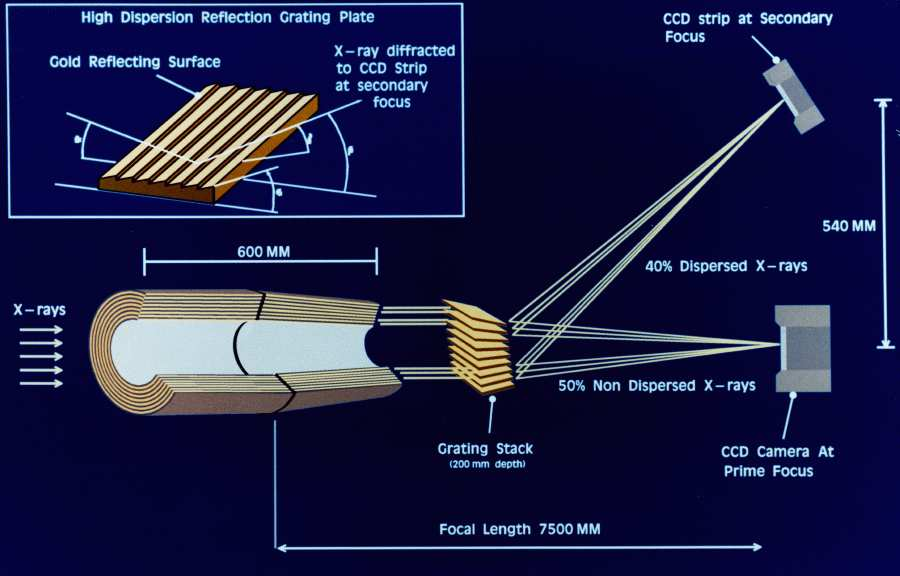
\includegraphics[width=0.9\textwidth]{xmm-rgs.png}
			\caption{Schematic of the RGS instruments of XMM-Newton. Courtesy: Hardware Schematics at XMM-Newton SOC}
			\label{xmm-rgs-instrument}
		\end{figure}
		
		\subsection{RGS Design and Functionality}			
			Each of the two XMM-Newton telescopes feeds light to a dedicated RGS instrument, referred to as RGS1 and RGS2, as illustrated in figure \ref{xmm-rgs-instrument} \footnote{\url{https://heasarc.gsfc.nasa.gov/docs/xmm/xmmhp_gal_hard_schem.html}}. These instruments consist of two main parts:
			\begin{enumerate}
				\item \textbf{Reflection Grating Assemblies (RGAs):} These assemblies act as the heart of the RGS instruments. They comprise arrays of precisely manufactured grating plates with microscopic grooves etched onto their surfaces, which play a crucial role in diffracting incoming X-ray photons. In figure \ref{xmm-rgs-instrument}, these are referred to as \emph{grating stack}.
				
				\item \textbf{RGS Focal Cameras (RFCs):} Downstream from the RGAs lie the RFCs. These consist of long, linear Charge-Coupled Device (CCD) detectors. The diffracted X-rays from the gratings fall onto these CCDs, where they are converted into electronic signals and ultimately into a digital spectrum. They are referred to as \emph{CCD strip} in figure \ref{xmm-rgs-instrument}.
			\end{enumerate}
		
			%The XMM-Newton satellite has three telescopes, out of which two are equipped with RGS instruments; these are referred to as RGS1 and RGS2. Each of these RGS instruments comprise of Reflection Grating Assemblies (RGAs) and RGS Focal Cameras (RFCs). These are referred to as \emph{grating stack} and \emph{CCD strip} in figure \ref{xmm-rgs-instrument}.
			
		\begin{table}[!htb]
			\centering
			\caption{In-orbit performance of RGS instruments}
			\label{xmm-rgs-performance}
			\begin{tabular}{l|l|ccc|ccc}
				\hline
				\multicolumn{2}{l|}{\multirow{2}{*}{\textbf{Parameter}}} & \multicolumn{3}{c|}{\textbf{RGS1}} & \multicolumn{3}{c}{\textbf{RGS2}} \\ \cline{3-8}
				\multicolumn{2}{l|}{} & {10 \AA} & {15 \AA} & {35 \AA} & {10 \AA} & {15 \AA} & {35 \AA} \\ \hline
				\multirow{2}{*}{Effective area (cm$^2$)} & {1$^\text{st}$ order} & {51} & {61} & {21} & {53} & {68} & {25} \\ %\cline{2-8}
														 & {2$^\text{nd}$ order} & {29} & {15} & {--} & {31} & {19} & {--} \\ \hline
				\multirow{2}{*}{Resolution (km s$^{-1}$)}& {1$^\text{st}$ order} & {1700} & {1200} & {600} & {1900} & {1400} & {700} \\ %\cline{2-8}
														 & {2$^\text{nd}$ order} & {1000} & {700} & {--} & {1200} & {800} & {--} \\ \hline
				\multirow{2}{*}{Wavelength range} & {1$^\text{st}$ order} & \multicolumn{6}{c}{5 -- 38 \AA (0.35 -- 2.5 keV)} \\ %\cline{2-8}
												   & {2$^\text{nd}$ order} & \multicolumn{6}{c}{5 -- 20 \AA (0.62 -- 2.5 keV)} \\ \hline
				\multirow{2}{*}{Wavelength accuracy} & {1$^\text{st}$ order} & \multicolumn{3}{c}{$\pm$5 m\AA} & \multicolumn{3}{c}{$\pm$5 m\AA} \\ %\cline{2-8}
                                                  	  & {2$^\text{nd}$ order} & \multicolumn{3}{c}{$\pm$4 m\AA} & \multicolumn{3}{c}{$\pm$3 m\AA} \\ \hline
				\multicolumn{2}{l|}{\multirow{2}{*}{Bin size {[}$3\times 3$ (27 $\mu$)$^2$ pixels{]}}} & \multicolumn{6}{c}{2.5 arcsec (cross dispersion direction)} \\ %\cline{3-8}
				\multicolumn{2}{l|}{} & \multicolumn{6}{c}{7 -- 14 m\AA (dispersion direction, first order)} \\ \hline
			\end{tabular}
		\end{table}
		
		\subsection{Light Path and Spectral Orders}
			%The light path of the two X-ray telescopes are focussed onto the EPIC MOS cameras at the primary focus. The RGAs intercept $\sim 58$ per cent of the light on the light path and diffracts it to the RFCs at the secondary focus. In order to diffract the light, the RGAs have grating plates with groove densities of $\sim 645.6$ lines mm$^{-1}$. This produces the two prominent first and second order spectra with dispersion of 8.3 and 12.7 mm \AA$^{-1}$ at 15 \AA. The performance of various parameters of the RGS instruments, while in orbit, are summarised in the table \ref{xmm-rgs-performance}.
			While the primary focus of the XMM-Newton telescopes is occupied by the European Photon Imaging Camera (EPIC) MOS detectors, designed for high-resolution X-ray imaging, the RGAs ingeniously intercept about 58 per cent of the incoming light before it reaches the EPIC cameras. This light then interacts with the grating plates in the RGAs. The gratings cause the X-ray photons to diffract, separating them according to their energy (wavelength). This phenomenon produces the two prominent first and second order spectra with dispersion of 8.3 and 12.7 mm \AA$^{-1}$ at 15 \AA.
			
			These spectral orders are dispersed across the length of the CCD strips, with higher energy (shorter wavelength) photons landing closer to the beginning of the CCD and lower energy (longer wavelength) photons landing towards the end. This creates a one-to-one mapping between position on the CCD and the energy (or wavelength) of the detected X-ray photon.
			
			The performance characteristics of the RGS instruments, as measured in orbit, are summarized in table \ref{xmm-rgs-performance}, which highlights key parameters namely the \textit{effective area}, \textit{resolution}, \textit{wavelength range}, \textit{wavelength accuracy} and \textit{bin size}.
	
			The effective area represents the collecting power of the instrument at a specific wavelength. As expected, the effective area is higher for the first order compared to the second. Resolution refers to the instrument's ability to distinguish between closely spaced spectral lines. Evidently, the resolution degrades at longer wavelengths (lower energies) within each order. The wavelength range covered by the RGS instruments allows them to probe a vast array of emission lines crucial for understanding the elemental composition and physical conditions within the X-ray emitting source.
			
			While higher-order spectra (beyond the first and second) are technically present, their count rates are significantly lower ($\sim 8$ times lower than that in the second order), rendering them less useful for scientific analysis. Consequently, processed scientific data products from the XMM-Newton Science Operations Centre (SOC) typically only include spectra from the first and second orders. Table \ref{xmm-rgs-wavelength} provides a concise overview of the wavelength and corresponding photon energy ranges covered by these two primary spectral orders.
			%The reflection grating used in the RGS instruments diffract into the first and second spectral orders with the highest efficiency -- therefore these two orders produce the most useful data. Even though the third order spectra are present, their count rates are $\sim 8$ times lower than that in the second order. Therefore, the science data provided by the XMM-Newton SOC consists of spectral data from first and second orders only. Table \ref{xmm-rgs-wavelength} summarises the wavelength range covered by the different spectral orders of the RGS instruments.
			\begin{table}[!htb]
				\centering
				\caption{Wavelength and photon energy ranges covered by RGS}
				\label{xmm-rgs-wavelength}
				\begin{tabular}{ccc}
					\hline
					{\textbf{Order}} & {\textbf{Wavelength range (\AA)}} & {\textbf{Photon energy range (keV)}} \\
					\hline
					{1} & {6 -- 38} & {0.3 -- 2.0} \\
					%\hline
					{2} & {6 -- 20} & {0.6 -- 2.0} \\
					\hline
				\end{tabular}
			\end{table}
	
	\section{\MakeUppercase{Models for Data Fitting}} \label{hi-resolution:models}
		The analysis of high-resolution X-ray spectra, such as those obtained with XMM-Newton RGS, involves a meticulous process of spectral fitting. This process aims to construct a mathematical model that accurately represents the observed spectrum, allowing us to extract meaningful physical information about the source.
		
		\subsection{Model Grid} \label{hi-resolution:models:grid}
			%Given below in table \ref{xmm-rgs-model-list} is the progression of Xspec models used in the analysis of the RGS spectrum of RX J0925.7-4758. Every model is given a model ID and hereinafter it will be referred to by the same. The progression of the models is evolutionary and follows the same sequence as each was built from the preceding model.
			Table \ref{xmm-rgs-model-list} presents a sequence of XSPEC models progressively employed to fit the RGS spectrum of the source RX J0925.7-4758. Each model builds upon the previous one, incorporating additional complexity or refining existing components. For instance, consider the initial model, i.e. M01. This model incorporates two components:
			\begin{enumerate}[i.]
				\item \texttt{tbabs}\footnote{\url{https://heasarc.gsfc.nasa.gov/xanadu/xspec/manual/node273.html}}: This is a multiplicative model component that accounts for the absorption of X-ray photons by the interstellar medium (ISM) along the line of sight to the source, by calculating the cross section for X-ray absorption as the sum of the cross sections for X-ray absorption due to the gas-phase ISM, the grain-phase ISM, and the molecules in the ISM \cite{wilms2000tbabs}.
				
				\item \texttt{bbody}\footnote{\url{https://heasarc.gsfc.nasa.gov/xanadu/xspec/manual/node136.html}} This is an additive model component which represents the intrinsic continuum emission from the source, modeled as a blackbody. Blackbody radiation describes the emission spectrum of a perfect thermal radiator, characterized by a single effective temperature.
			\end{enumerate}
			
			\begin{table}[!htb]
				\centering
				\caption{List of models used for RGS data fitting for \source}
				\label{xmm-rgs-model-list}
				\begin{tabular}{lll}
					\hline
					\textbf{S. No.} & \textbf{Model ID} & \textbf{Xspec model} \\ \hline
					{1} & {M01} & \texttt{tbabs*bbody} \\ %\hline
					{2} & {M02} & \texttt{ismabs*bbody} \\ %\hline
					{3} & {M03} & \texttt{ismabs*(gauss+bbody)} \\ %\hline
					{4} & {M04} & \texttt{ismabs*edge$^3$*(gauss+bbody)} \\ %\hline
					{5} & {M05} & \texttt{ismabs*edge$^3$*(mekal+bbody)} \\ %\hline
					{6} & {M06} & \texttt{ismabs*(apec+mekal)*swind1} \\ %\hline
					{7} & {M07} & \texttt{ismabs*(gauss+mekal+bbody)} \\ %\hline
					{8} & {M08} & \texttt{ismabs*(gauss+mekal+bbody)*swind1} \\ %\hline
					{9} & {M09} & \texttt{ismabs*(rauch+mekal)*swind1} \\ %\hline
					{10} & {M10} & \texttt{ismabs*(rauch+apec)*swind1} \\ %\hline
					{11} & {M11} & \texttt{ismabs*(rauch*tbabs+apec+mekal)*swind1} \\ %\hline
					{12} & {M12} & \texttt{ismabs*(rauch+apec+mekal)*swind1} \\ \hline
				\end{tabular}
			\end{table}
			
			By multiplying tbabs with bbody, the model M01 essentially takes the intrinsic blackbody emission (\texttt{bbody}) and modifies it according to the absorption characteristics of the intervening ISM (\texttt{tbabs}).  This allows for a preliminary fit to the observed spectrum, accounting for both the source's emission and the dimming effect of the interstellar medium. While this model provides a basic framework,  it's often too simplistic for complex X-ray sources. Real celestial objects might exhibit additional features like emission lines, multiple thermal components, or non-thermal emission processes. Subsequent models incorporate these complexities to achieve a more accurate representation of the observed spectrum.
			
			The subsequent models become progressively more complex, incorporating additional components to capture the intricate features of the RGS spectrum. The final models (M11 and M12) exhibit the most intricate structure, potentially accounting for multiple sources of absorption (represented by the combination of rauch and tbabs within M11) and a complex interplay of thermal emission processes (involving both mekal and apec components).
			
			By systematically refining the model through this iterative process of adding and adjusting components, we have tried to achieve the best possible fit to the observed spectrum. The quality of the fit is typically evaluated using statistical tests, and the resulting model parameters provide crucial insights into the physical properties of the X-ray emitting source and its environment.
	  
			% is a simple model which is composed of two model components -- an additive component (\texttt{bbody}) and a multiplicative component (\texttt{tbabs}). This particular model was mainly used to get started with the modelling of the continuum spectrum using a blackbody emission, subjected to absorption. Then, as one progresses downwards along table \ref{xmm-rgs-model-list}, one finds models which are improvements upon the previous model, in terms of the replacement of existing model components or the addition of newer ones.
	
		\subsection{Model Components} \label{hi-resolution:models:components}
			XSPEC allows one to construct complex models of astronomical spectra by combining simpler ones. These simpler models represent various physical processes that contribute to the overall observed spectrum. This section describes some the model components utilised to construct the model grid, as described in \S\ \ref{hi-resolution:models:grid}.
		
			\subsubsection{X-ray Photoabsorption Model: \texttt{ismabs}}
			The \texttt{ismabs} multiplicative model in Xspec provides a way to simulate X-ray photoabsorption \cite{gatuzz2015ismabs}. This model incorporates variable columns for both neutral and ionized species from H, He, N, O, Ne, Mg, Si, S, Ar, Ca, Fe, Ni and Zn.
			
			Because of an inherent degeneracy between the relative columns of H, He I, He II, the column density of He I is not included as a free parameter in the model.
			
			In this model, the absorption cross-sections for various species are sourced as follows:
			\begin{itemize}
				\item Neutral states of Si, S, Ar and Ca from Verner \etal\ \cite{vernerXS}
				\item Singly and doubly ionized states of Si, S, Ar and Ca from Witthoeft \etal\ \cite{witthoeftXS1,witthoeftXS2}
				\item Neutral, singly and doubly ionized states of N from Garcia \etal\ \cite{garciaXS1}
				\item Neutral states of O from Gorczyca \etal\ \cite{gorczycaXS1}
				\item Singly and doubly ionized states of O from Garcia \etal\ \cite{garciaXS2}, including corrections applied by Gatuzz \etal\ \cite{gatuzzXS}
				\item Neutral state of Ne from Gorczyca \etal\ \cite{gorczycaXS2}
				\item Singly and doubly ionized states of Ne from Gorczyca \etal\ \cite{gorczycaXS3}
				\item For the Fe-L edge region we use the measurement of metallic iron by Kortright and Kim \cite{kortrightXS}
				\item Neutral, singly and doubly ionized states of Mg from Hasoglu \etal\ (2014).
			\end{itemize}
			
			The parameters for the \texttt{ismabs} model are given in table \ref{param:ismabs}.
			\begin{table}[h!]
				\centering
				\caption{Model parameters for \texttt{ismabs}}
				\label{param:ismabs}
				\begin{tabular}{p{0.13\textwidth}p{0.32\textwidth}|p{0.13\textwidth}p{0.32\textwidth}}
					\hline
					\textbf{Parameter} & \textbf{Quantity} & \textbf{Parameter} & \textbf{Quantity} \\ \hline
					{\texttt{par1}} & {H col. (in $10^{22}$ cm$^{-2}$)} & {\texttt{par2}} & {He II col. (in $10^{22}$ cm$^{-2}$)} \\ %\hline
					{\texttt{par3}} & {C I col. (in $10^{22}$ cm$^{-2}$)} & {\texttt{par4}} & {C II col. (in $10^{22}$ cm$^{-2}$)} \\ %\hline
					{\texttt{par5}} & {C III col. (in $10^{22}$ cm$^{-2}$)} & {\texttt{par6}} & {N I col. (in $10^{22}$ cm$^{-2}$)} \\ %\hline
					{\texttt{par7}} & {N II col. (in $10^{22}$ cm$^{-2}$)} & {\texttt{par8}} & {N III col. (in $10^{22}$ cm$^{-2}$)} \\ %\hline
					{\texttt{par9}} & {O I col. (in $10^{22}$ cm$^{-2}$)} & {\texttt{par10}} & {O II col. (in $10^{22}$ cm$^{-2}$)} \\ %\hline
					{\texttt{par11}} & {O III col. (in $10^{22}$ cm$^{-2}$)} & {\texttt{par12}} & {Ne I col. (in $10^{22}$ cm$^{-2}$)} \\ %\hline
					{\texttt{par13}} & {Ne II col. (in $10^{22}$ cm$^{-2}$)} & {\texttt{par14}} & {Ne III col. (in $10^{22}$ cm$^{-2}$)} \\ %\hline
					{\texttt{par15}} & {Mg I col. (in $10^{22}$ cm$^{-2}$)} & {\texttt{par16}} & {Mg II col. (in $10^{22}$ cm$^{-2}$)} \\ %\hline
					{\texttt{par17}} & {Mg III col. (in $10^{22}$ cm$^{-2}$)} & {\texttt{par18}} & {Si I col. (in $10^{22}$ cm$^{-2}$)} \\ %\hline
					{\texttt{par19}} & {Si II col. (in $10^{22}$ cm$^{-2}$)} & {\texttt{par20}} & {Si III col. (in $10^{22}$ cm$^{-2}$)} \\ %\hline
					{\texttt{par21}} & {S I col. (in $10^{22}$ cm$^{-2}$)} & {\texttt{par22}} & {S II col. (in $10^{22}$ cm$^{-2}$)} \\ %\hline
					{\texttt{par23}} & {S III col. (in $10^{22}$ cm$^{-2}$)} & {\texttt{par24}} & {Ar I col. (in $10^{22}$ cm$^{-2}$)} \\ %\hline
					{\texttt{par25}} & {Ar II col. (in $10^{22}$ cm$^{-2}$)} & {\texttt{par26}} & {Ar III col. (in $10^{22}$ cm$^{-2}$)} \\ %\hline
					{\texttt{par27}} & {Ca I col. (in $10^{22}$ cm$^{-2}$)} & {\texttt{par28}} & {Ca II col. (in $10^{22}$ cm$^{-2}$)} \\ %\hline
					{\texttt{par29}} & {Ca III col. (in $10^{22}$ cm$^{-2}$)} & {\texttt{par30}} & {Fe col. (in $10^{22}$ cm$^{-2}$)} \\ %\hline
					{\texttt{par31}} & {Redshift $z$} & {} & {} \\ \hline
				\end{tabular}
			\end{table}
			
			\subsubsection{Astrophysical Plasma Emission Code: \texttt{apec}}
				The \texttt{apec} additive model in Xspec simulates an emission spectrum that is obtained from a collisionally-ionized diffuse gas \cite{smithAPEC}. The atomic data for collisional and radiative rates, recombination cross sections, dielectronic recombination rates, and satellite line wavelengths are taken from the Astrophysical Plasma Emission Database (APED).
			
				The \texttt{apec} model provides a way to create emission models for plasma, which can be used to analyse spectral data from high-resolution X-ray spectrometers, as in the case of XMM-Newton or Chandra. The current version of the code stores the atomic data in FITS files, thereby separating it from the code. This optimizes limitations on the speed and memory across different computers.
			
				The \texttt{apec} model simulates a hot, optically thin plasma which is in a collisional ionization equilibrium, and computes both resulting continuum and line emissivities. Here, the \textit{emissivity} of a spectral line is defined as the  total number of radiative transitions per unit volume divided by the product of the electron density $n_e$ and the hydrogen (neutrals and protons) density $n_H$ in the astrophysical plasma, resulting in line emissivities having units of cm$^3$ s$^{-1}$.
			
				The parameters for the \texttt{apec} model are given in table \ref{param:apec}.
				\begin{table}[h!]
					\centering
					\caption{Model parameters for \texttt{apec}}
					\label{param:apec}
					\begin{tabular}{p{0.2\textwidth}p{0.7\textwidth}}
						\hline
						\textbf{Parameter} & \textbf{Quantity} \\ \hline
						{\texttt{par1}} & {Plasma temperature (in keV)} \\ %\hline
						{\texttt{par2}} & {Abundances of the metals C, N, O, Ne, Mg, Al, Si, S, Ar, Ca, Fe, Ni} \\ %\hline
						{\texttt{par3}} & {Redshift $z$} \\ %\hline
						{\texttt{norm}} & {Normalization of the component computed as $\displaystyle\dfrac{10^{-14}}{4\pi[D_A(1+z)]^2}\int{n_en_H\diff{V}}$, where $D_A$ is the angular diameter distance to the source (in cm), $n_e$ and $n_H$ are the electron densities (in cm$^{-3}$) respectively} \\ \hline
					\end{tabular}
				\end{table}

			\subsubsection{Model for Emission Due to Optically-Thin Plasma: \texttt{mekal}}
				The additive model \texttt{mekal} in Xspec allows the simulation of an emission spectrum due to a diffuse plasma, whose electrons have a Maxwellian energy distribution. This model uses the spectral line list as calculated by Mewe and Kaastra \cite{meka}, additional calculations for L-shell of Fe ions by Liedahl \etal\ \cite{liedahl}. The model provides the option to either calculate the spectrum by running the \texttt{mekal} code, or by interpolation on a pre-calculated \texttt{mekal} table, or simply by using the AtomDB data.
				
				The models \texttt{mekal} and \texttt{apec} both simulate emission due to optically-thin plasma, the difference being in the methodology of calculation of the line lists.
				
				The parameters for the \texttt{mekal} model are given in table \ref{param:mekal}.
				\begin{table}[h!]
					\centering
					\caption{Model parameters for \texttt{mekal}}
					\label{param:mekal}
					\begin{tabular}{p{0.2\textwidth}p{0.7\textwidth}}
						\hline
						\textbf{Parameter} & \textbf{Quantity} \\ \hline
						{\texttt{par1}} & {Plasma temperature (in keV)} \\ %\hline
						{\texttt{par2}} & {H density (in cm$^{-3}$)} \\ %\hline
						{\texttt{par3}} & {Metal abundances for the elements C, N, O, Ne, Na, Mg, Al, Si, S, Ar, Ca, Fe, Ni} \\ %\hline
						{\texttt{par4}} & {Redshift $z$} \\ %\hline
						{\texttt{par5}} & {Switch between \texttt{mekal} calculation (0), interpolation (1) and interpolation using AtomDB data (2)} \\ %\hline
						{\texttt{norm}} & {Normalization of the component computed as $\displaystyle\dfrac{10^{-14}}{4\pi[D_A(1+z)]^2}\int{n_en_H\diff{V}}$, where $D_A$ is the angular diameter distance to the source (in cm), $n_e$ and $n_H$ are the electron densities (in cm$^{-3}$) respectively} \\ \hline
					\end{tabular}
				\end{table}
			
			\subsubsection{Velocity Shear Absorption: \texttt{swind1}}
				Originally meant for AGN spectra, the \texttt{swind1} multiplicative model fits the soft excess in partially ionized absorbing material with a large velocity shear. This is approximated by the model component by using XSTAR kn5 photoionization absorption model grids, which were calculated assuming a micro-turbulence of 100 km/s, and subsequently convolving with Gaussian smearing \cite{swind1}.
				
				In this work, the \texttt{swind1} component is used as a proxy model for possible stellar wind from the source RX J0925.7-4758, which may be indicated by the presence of P Cygni profiles in its spectrum.
				
				The parameters for the \texttt{swind1} model are given in table \ref{param:swind1}.
				\begin{table}[h!]
					\centering
					\caption{Model parameters for \texttt{swind1}}
					\label{param:swind1}
					\begin{tabular}{p{0.2\textwidth}p{0.7\textwidth}}
						\hline
						\textbf{Parameter} & \textbf{Quantity} \\ \hline
						{\texttt{par1}} & {Column density (in $10^{22}$ cm$^{-2}$)} \\ %\hline
						{\texttt{par2}} & {$\log{\xi}$ where $\xi=L/nr^2$} \\ %\hline
						{\texttt{par3}} & {$\sigma$: Gaussian $\sigma$ for velocity smearing ($v/c$)} \\ %\hline
						{\texttt{par4}} & {Redshift $z$} \\ \hline
					\end{tabular}
				\end{table}
			
			\subsubsection{T\"{u}bingen NLTE Model-Atmosphere Package: \texttt{rauch}}
				The T\"{u}bingen NLTE Model-Atmosphere Package (TMAP) is a tool to calculate stellar atmospheres in spherical or plane-parallel geometry in hydrostatic and radiative equilibrium allowing departures from local thermodynamic equilibrium (LTE) for the population of atomic levels \cite{werner1999classical}. TMAP is based on the so-called Accelerated Lambda Iteration (ALI) method and is able to account for line blanketing by metals \cite{rauchALI}. All elements from hydrogen to nickel may be included in the calculation with model atoms which are tailored for the aims of the user \cite{wernerTMAP}.
				
				The web-link to a set of theoretical spectral energy distributions (SEDs) of TMAP NLTE model atmospheres were provided by Rauch \cite{rauchFITS}, which contained a grid of 10 FITS files for varying temperatures. The abundances of various elements for this grid are given in table \ref{rauch:abundances}. The TMAP model series refer to the files corresponding to the model atmosphere grid, with each column named after the last three characters of the FITS filename. The grid is calculated for effective temperatures in the range $4.50\times 10^5\,\text{K}\leqslant T_\text{eff}\leqslant 1.05\times 10^6\,\text{K}$ in steps $\Delta T=10^4\,\text{K}$. The effective surface gravity is $\log_{10}{g}=9$. The fluxes in the SEDs are calculated using the TMAP code from models with different elemental abundance ratios $[X]$.
				
%				\begin{table}[h!]
%					\centering
%					\caption{Elemental abundances for TMAP grid}
%					\label{rauch:abundances}
%					\begin{tabular}{|c|cccccccccc|}
%						\hline
%						\multirow{2}{*}{\textbf{{[}X{]}}} & \multicolumn{10}{c|}{\textbf{TMAP model series}} \\ \cline{2-11} & \multicolumn{1}{c|}{\textbf{003}} & \multicolumn{1}{c|}{\textbf{004}} & \multicolumn{1}{c|}{\textbf{005}} & \multicolumn{1}{c|}{\textbf{006}} & \multicolumn{1}{c|}{\textbf{007}} & \multicolumn{1}{c|}{\textbf{008}} & \multicolumn{1}{c|}{\textbf{009}} & \multicolumn{1}{c|}{\textbf{010}} & \multicolumn{1}{c|}{\textbf{011}} & \textbf{201} \\ \hline
%						{[}H{]} & \multicolumn{1}{c|}{-0.688} & \multicolumn{1}{c|}{-0.683} & \multicolumn{1}{c|}{-0.677} & \multicolumn{1}{c|}{-0.673} & \multicolumn{1}{c|}{-0.672} & \multicolumn{1}{c|}{-0.671} & \multicolumn{1}{c|}{-0.670} & \multicolumn{1}{c|}{-0.670} & \multicolumn{1}{c|}{-0.669} & -0.885 \\ \hline
%						{[}He{]} & \multicolumn{1}{c|}{0.382} & \multicolumn{1}{c|}{0.387} & \multicolumn{1}{c|}{0.393} & \multicolumn{1}{c|}{0.397} & \multicolumn{1}{c|}{0.398} & \multicolumn{1}{c|}{0.399} & \multicolumn{1}{c|}{0.400} & \multicolumn{1}{c|}{0.401} & \multicolumn{1}{c|}{0.401} & 0.489 \\ \hline
%						{[}C{]} & \multicolumn{1}{c|}{-1.513} & \multicolumn{1}{c|}{-1.073} & \multicolumn{1}{c|}{-0.772} & \multicolumn{1}{c|}{-0.675} & \multicolumn{1}{c|}{-0.596} & \multicolumn{1}{c|}{-0.529} & \multicolumn{1}{c|}{-0.471} & \multicolumn{1}{c|}{-0.420} & \multicolumn{1}{c|}{-0.374} & -0.057 \\ \hline
%						{[}N{]} & \multicolumn{1}{c|}{1.803} & \multicolumn{1}{c|}{1.678} & \multicolumn{1}{c|}{1.460} & \multicolumn{1}{c|}{1.159} & \multicolumn{1}{c|}{1.062} & \multicolumn{1}{c|}{0.937} & \multicolumn{1}{c|}{0.761} & \multicolumn{1}{c|}{0.460} & \multicolumn{1}{c|}{0.159} & 1.668 \\ \hline
%						{[}O{]} & \multicolumn{1}{c|}{1.528} & \multicolumn{1}{c|}{1.533} & \multicolumn{1}{c|}{1.538} & \multicolumn{1}{c|}{1.543} & \multicolumn{1}{c|}{1.544} & \multicolumn{1}{c|}{1.544} & \multicolumn{1}{c|}{1.545} & \multicolumn{1}{c|}{1.546} & \multicolumn{1}{c|}{1.547} & 1.206 \\ \hline
%						{[}Ne{]} & \multicolumn{1}{c|}{-0.474} & \multicolumn{1}{c|}{-0.469} & \multicolumn{1}{c|}{-0.464} & \multicolumn{1}{c|}{-0.459} & \multicolumn{1}{c|}{-0.459} & \multicolumn{1}{c|}{-0.458} & \multicolumn{1}{c|}{-0.457} & \multicolumn{1}{c|}{-0.456} & \multicolumn{1}{c|}{-0.456} & -0.517 \\ \hline
%						{[}Mg{]} & \multicolumn{1}{c|}{-0.454} & \multicolumn{1}{c|}{-0.450} & \multicolumn{1}{c|}{-0.444} & \multicolumn{1}{c|}{-0.439} & \multicolumn{1}{c|}{-0.439} & \multicolumn{1}{c|}{-0.438} & \multicolumn{1}{c|}{-0.437} & \multicolumn{1}{c|}{-0.436} & \multicolumn{1}{c|}{-0.436} & -0.497 \\ \hline
%						{[}Si{]} & \multicolumn{1}{c|}{0.167} & \multicolumn{1}{c|}{0.172} & \multicolumn{1}{c|}{0.178} & \multicolumn{1}{c|}{0.182} & \multicolumn{1}{c|}{0.183} & \multicolumn{1}{c|}{0.184} & \multicolumn{1}{c|}{0.185} & \multicolumn{1}{c|}{0.186} & \multicolumn{1}{c|}{0.186} & 0.125 \\ \hline
%						{[}S{]} & \multicolumn{1}{c|}{-1.583} & \multicolumn{1}{c|}{-1.578} & \multicolumn{1}{c|}{-1.573} & \multicolumn{1}{c|}{-1.568} & \multicolumn{1}{c|}{-1.567} & \multicolumn{1}{c|}{-1.567} & \multicolumn{1}{c|}{-1.566} & \multicolumn{1}{c|}{-1.565} & \multicolumn{1}{c|}{-1.565} & -1.625 \\ \hline
%						{[}IG{]} & \multicolumn{1}{c|}{0.828} & \multicolumn{1}{c|}{0.833} & \multicolumn{1}{c|}{0.838} & \multicolumn{1}{c|}{0.843} & \multicolumn{1}{c|}{0.843} & \multicolumn{1}{c|}{0.844} & \multicolumn{1}{c|}{0.845} & \multicolumn{1}{c|}{0.846} & \multicolumn{1}{c|}{0.846} & 0.786 \\ \hline
%					\end{tabular}
%				\end{table}
				
				\begin{table}[h!]
					\centering
					\caption{Elemental abundances for TMAP grid}
					\label{rauch:abundances}
					\begin{tabular}{ccccccccccc}
						\hline
						\multirow{2}{*}{\textbf{{[}X{]}}} & \multicolumn{10}{c}{\textbf{TMAP model series}} \\ \cline{2-11} & \multicolumn{1}{c}{\textbf{003}} & \multicolumn{1}{c}{\textbf{004}} & \multicolumn{1}{c}{\textbf{005}} & \multicolumn{1}{c}{\textbf{006}} & \multicolumn{1}{c}{\textbf{007}} & \multicolumn{1}{c}{\textbf{008}} & \multicolumn{1}{c}{\textbf{009}} & \multicolumn{1}{c}{\textbf{010}} & \multicolumn{1}{c}{\textbf{011}} & \textbf{201} \\ \hline
						{[}H{]} & \multicolumn{1}{c}{-0.688} & \multicolumn{1}{c}{-0.683} & \multicolumn{1}{c}{-0.677} & \multicolumn{1}{c}{-0.673} & \multicolumn{1}{c}{-0.672} & \multicolumn{1}{c}{-0.671} & \multicolumn{1}{c}{-0.670} & \multicolumn{1}{c}{-0.670} & \multicolumn{1}{c}{-0.669} & -0.885 \\ %\hline
						{[}He{]} & \multicolumn{1}{c}{0.382} & \multicolumn{1}{c}{0.387} & \multicolumn{1}{c}{0.393} & \multicolumn{1}{c}{0.397} & \multicolumn{1}{c}{0.398} & \multicolumn{1}{c}{0.399} & \multicolumn{1}{c}{0.400} & \multicolumn{1}{c}{0.401} & \multicolumn{1}{c}{0.401} & 0.489 \\ %\hline
						{[}C{]} & \multicolumn{1}{c}{-1.513} & \multicolumn{1}{c}{-1.073} & \multicolumn{1}{c}{-0.772} & \multicolumn{1}{c}{-0.675} & \multicolumn{1}{c}{-0.596} & \multicolumn{1}{c}{-0.529} & \multicolumn{1}{c}{-0.471} & \multicolumn{1}{c}{-0.420} & \multicolumn{1}{c}{-0.374} & -0.057 \\ %\hline
						{[}N{]} & \multicolumn{1}{c}{1.803} & \multicolumn{1}{c}{1.678} & \multicolumn{1}{c}{1.460} & \multicolumn{1}{c}{1.159} & \multicolumn{1}{c}{1.062} & \multicolumn{1}{c}{0.937} & \multicolumn{1}{c}{0.761} & \multicolumn{1}{c}{0.460} & \multicolumn{1}{c}{0.159} & 1.668 \\ %\hline
						{[}O{]} & \multicolumn{1}{c}{1.528} & \multicolumn{1}{c}{1.533} & \multicolumn{1}{c}{1.538} & \multicolumn{1}{c}{1.543} & \multicolumn{1}{c}{1.544} & \multicolumn{1}{c}{1.544} & \multicolumn{1}{c}{1.545} & \multicolumn{1}{c}{1.546} & \multicolumn{1}{c}{1.547} & 1.206 \\ %\hline
						{[}Ne{]} & \multicolumn{1}{c}{-0.474} & \multicolumn{1}{c}{-0.469} & \multicolumn{1}{c}{-0.464} & \multicolumn{1}{c}{-0.459} & \multicolumn{1}{c}{-0.459} & \multicolumn{1}{c}{-0.458} & \multicolumn{1}{c}{-0.457} & \multicolumn{1}{c}{-0.456} & \multicolumn{1}{c}{-0.456} & -0.517 \\ %\hline
						{[}Mg{]} & \multicolumn{1}{c}{-0.454} & \multicolumn{1}{c}{-0.450} & \multicolumn{1}{c}{-0.444} & \multicolumn{1}{c}{-0.439} & \multicolumn{1}{c}{-0.439} & \multicolumn{1}{c}{-0.438} & \multicolumn{1}{c}{-0.437} & \multicolumn{1}{c}{-0.436} & \multicolumn{1}{c}{-0.436} & -0.497 \\ %\hline
						{[}Si{]} & \multicolumn{1}{c}{0.167} & \multicolumn{1}{c}{0.172} & \multicolumn{1}{c}{0.178} & \multicolumn{1}{c}{0.182} & \multicolumn{1}{c}{0.183} & \multicolumn{1}{c}{0.184} & \multicolumn{1}{c}{0.185} & \multicolumn{1}{c}{0.186} & \multicolumn{1}{c}{0.186} & 0.125 \\ %\hline
						{[}S{]} & \multicolumn{1}{c}{-1.583} & \multicolumn{1}{c}{-1.578} & \multicolumn{1}{c}{-1.573} & \multicolumn{1}{c}{-1.568} & \multicolumn{1}{c}{-1.567} & \multicolumn{1}{c}{-1.567} & \multicolumn{1}{c}{-1.566} & \multicolumn{1}{c}{-1.565} & \multicolumn{1}{c}{-1.565} & -1.625 \\ %\hline
						{[}IG{]} & \multicolumn{1}{c}{0.828} & \multicolumn{1}{c}{0.833} & \multicolumn{1}{c}{0.838} & \multicolumn{1}{c}{0.843} & \multicolumn{1}{c}{0.843} & \multicolumn{1}{c}{0.844} & \multicolumn{1}{c}{0.845} & \multicolumn{1}{c}{0.846} & \multicolumn{1}{c}{0.846} & 0.786 \\ \hline
					\end{tabular}
				\end{table}
				
				The quantity $[X]$ is logarithmic and is calculated as
				\begin{align}
					\label{rauch:[X]}
					[X]=\log{\left(\dfrac{\text{stellar mass fraction}}{\text{solar mass fraction}}\right)}=\log{\left(\dfrac{X_*}{X_\odot}\right)}
				\end{align}
				
				For any element $X$ denotes its mass fraction which is defined as $X\equiv\dfrac{m_X}{M}$, where $m_X$ is the mass of the element and $M$ is the total mass of the system. For example in table \ref{rauch:abundances},
				\begin{align*}
					[X]&=-0.675 \\
					\implies \log_{10}\left(\dfrac{X_*}{X_\odot}\right)&=-0.675 \\
					\implies \dfrac{X_*}{X_\odot}&=10^{-0.675} \\
					\implies X_*&=0.211X_\odot
				\end{align*}
				That is, $[X]$ indicates that the stellar mass fraction $X_*$ for that element is about 21 per cent that of solar mass fraction $X_\odot$.
				
				The parameters for the \texttt{rauch} model are given in table \ref{param:rauch}.
				\begin{table}[h!]
					\centering
					\caption{Model parameters for \texttt{rauch}}
					\label{param:rauch}
					\begin{tabular}{p{0.2\textwidth}p{0.7\textwidth}}
						\hline
						\textbf{Parameter} & \textbf{Quantity} \\ \hline
						{\texttt{par1}} & {Effective temperature $T$ (in K)} \\ %\hline
						{\texttt{par2}} & {Redshift $z$} \\ %\hline
						{\texttt{norm}} & {Normalization of the component computed as $\displaystyle\dfrac{10^{-14}}{4\pi[D_A(1+z)]^2}\int{n_en_H\diff{V}}$, where $D_A$ is the angular diameter distance to the source (in cm), $n_e$ and $n_H$ are the electron densities (in cm$^{-3}$) respectively} \\ \hline
					\end{tabular}
				\end{table}
	
	\section{\MakeUppercase{Analysis of High-resolution RGS Spectra}} \label{hi-resolution:analysis}
		The spectra of RX J0925.7-4758 obtained by both of the RGS instrument of XMM-Newton were analyzed using a subset of models from the list given in table \ref{xmm-rgs-model-list}. Models with IDs M07, M08, M09, M10, M11 and M12 were applied on the RGS data for both spectral orders.
		
		\subsection{Fitting of RGS1 Spectra} \label{hi-resolution:analysis:rgs1}
		
			\begin{figure}[h!]
				\centering
				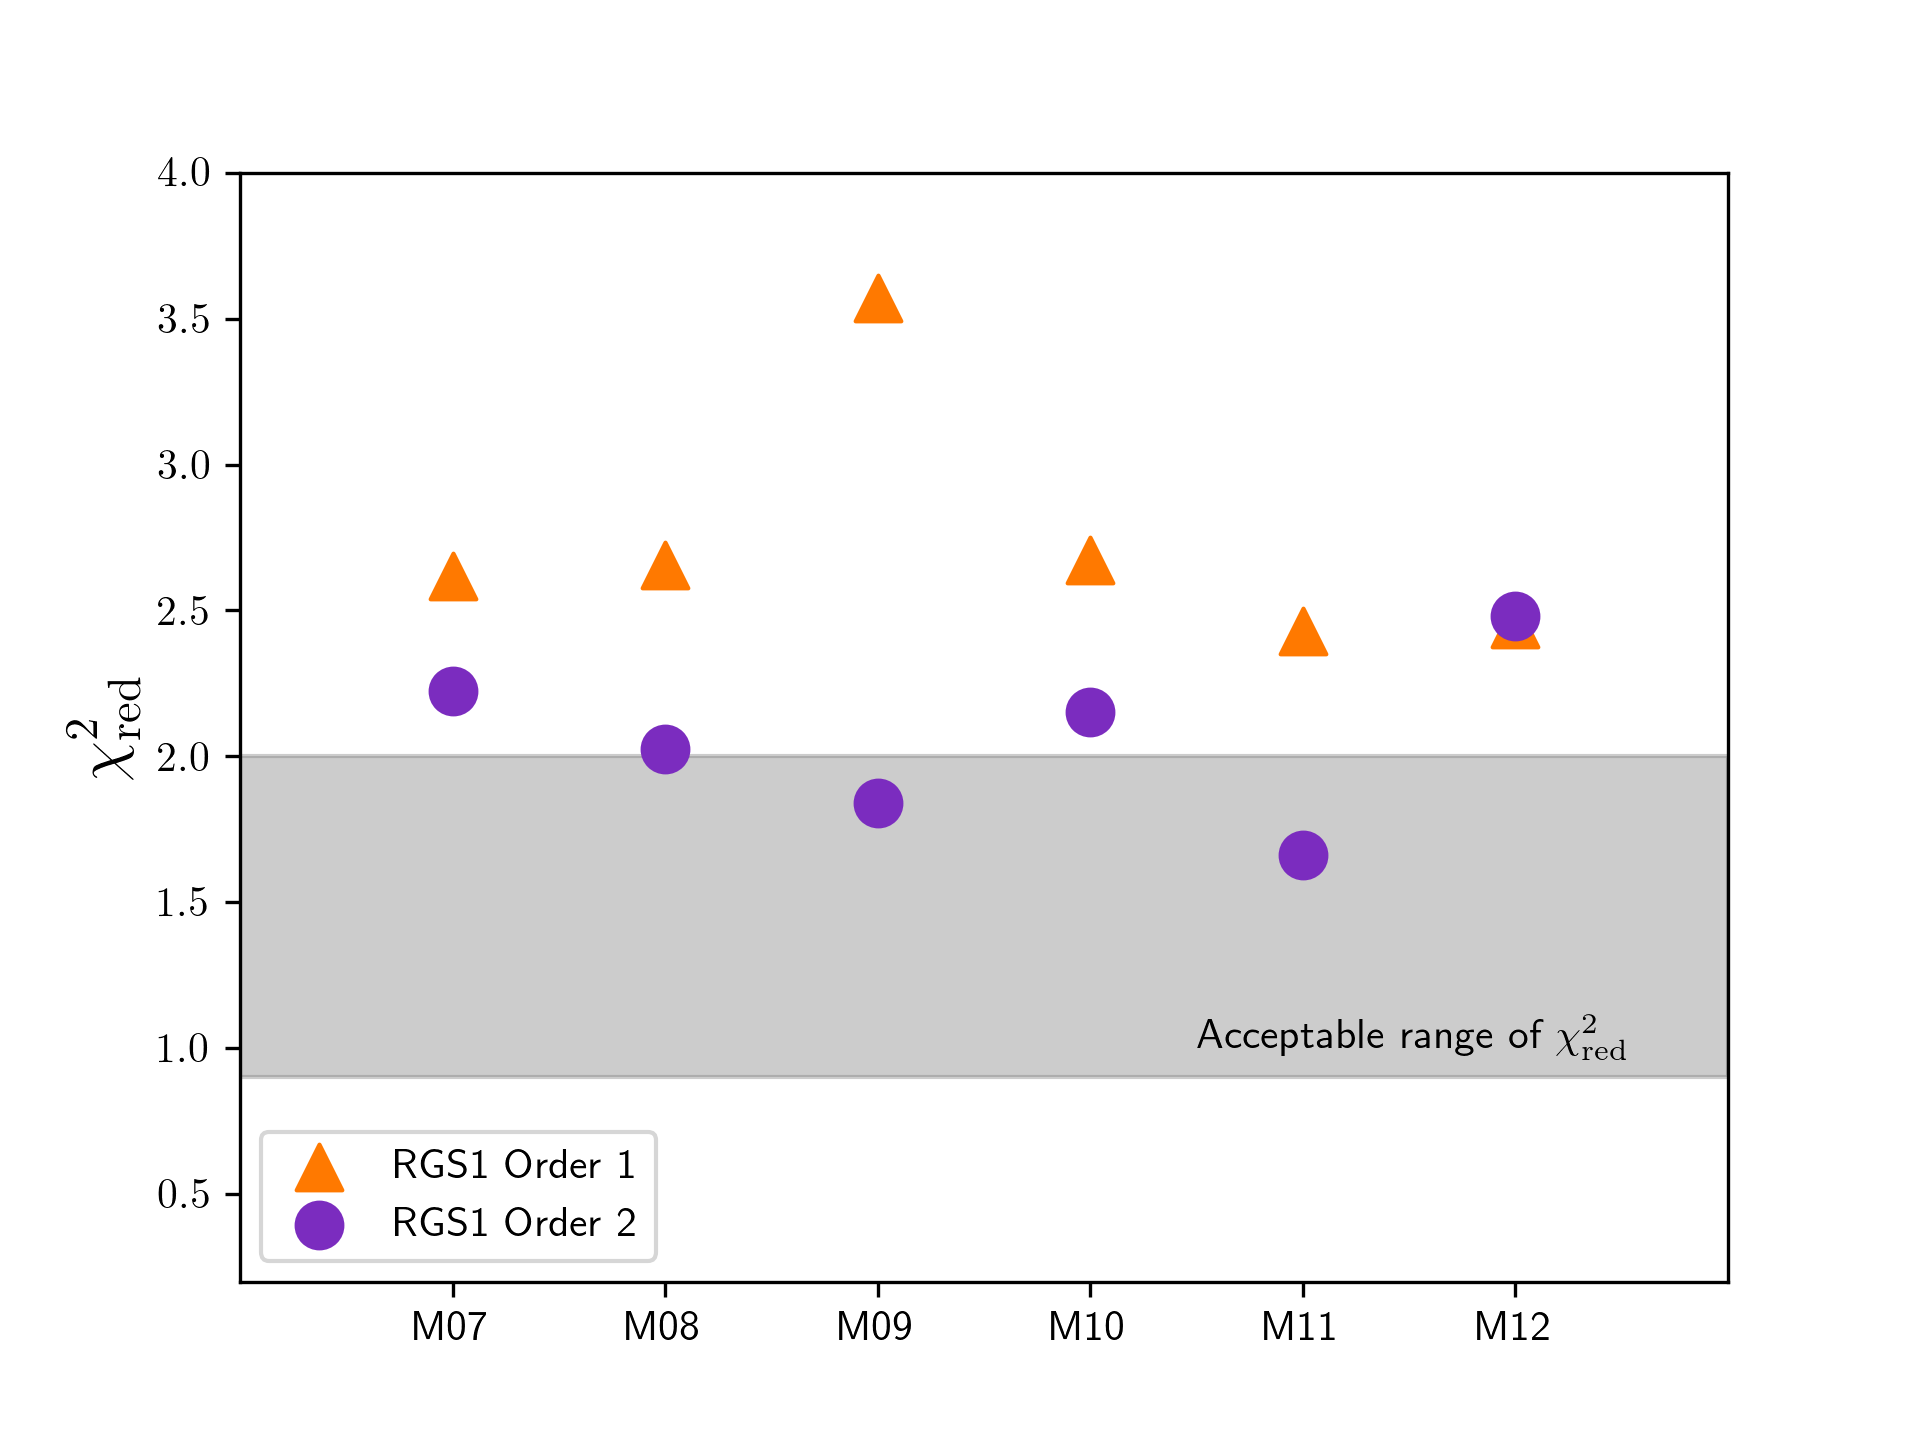
\includegraphics[width=\textwidth]{mrvel-rgs1-chisq_new}
				\caption{$\chi^2_\text{red}$ trend of RGS1 spectra from RX J0925.7-4758}
				\label{fig:mrvel-rgs1-chisq}
			\end{figure}
			
			We present here the results of fitting a selection of spectral models to the RGS1 data from RX J0925.7-4758. We assess the quality of each fit using the values of the reduced chi-squared statistic ($\chi^2_\text{reduced}$). Acceptable models typically have $\chi^2_\text{reduced}$ values in the range of 1 to 2. The fitting statistics are summarized in table \ref{tab:fit-stat:rgs1}.  These values are also plotted in figure \ref{fig:mrvel-rgs1-chisq} to visually identify models with acceptable $\chi^2_\text{reduced}$ values.
			%The fitting statistics obtained by fitting the selected subset of the model grid are summarized in table \ref{tab:fit-stat:rgs1}. The values of fitting statistics are plotted in figure \ref{fig:mrvel-rgs1-chisq} so as to graphically indicate the models whose $\chi^2_\text{reduced}$ values lie within the acceptable range of $(1,2)$.
			\begin{table}[!htb]
				\centering
				\caption{Fitting statistics of RGS1 spectra from RX J0925.7-4758}
				\label{tab:fit-stat:rgs1}
				\begin{tabular}{c|cc|cc}
					\hline
					\multirow{2}{*}{\textbf{Model ID}} & \multicolumn{2}{c|}{\textbf{RGS 1 $\vert$ Order 1}} & \multicolumn{2}{c}{\textbf{RGS 1 $\vert$ Order 2}} \\ \cline{2-5} & {$\boldsymbol{\chi^2}$/\textbf{d.o.f}} & {$\boldsymbol{\chi^2_\text{reduced}}$} & {$\boldsymbol{\chi^2}$/\textbf{d.o.f}} & {$\boldsymbol{\chi^2_\text{reduced}}$} \\ \hline
					{M07} & {1168.4/446} & {2.62} & {386.8/174} & {2.22} \\
					{M08} & {1176.8/443} & {2.66} & {346.4/171} & {2.03} \\
					{M09} & {1126.5/445} & {3.57} & {318.4/173} & {1.84} \\
					{M10} & {1194.4/445} & {2.68} & {372.4/173} & {2.15} \\
					{M11} & {1044.4/442} & {2.36} & {282.8/170} & {1.66} \\
					{M12} & {1087.5/443} & {2.45} & {424.2/171} & {2.48} \\ \hline
				\end{tabular}
			\end{table}
			
			As evident from table \ref{tab:fit-stat:rgs1} or figure \ref{fig:mrvel-rgs1-chisq}, the model M11 provides the best fit for both spectral orders.
			%This model can be written mathematically as: \\ \texttt{ismabs*(rauch*tbabs+apec+mekal)*swind1}
%			\begin{center}
%				\texttt{ismabs*(rauch*tbabs+apec+mekal)*swind1}
%			\end{center}			
			While other models do not yield the best fit according to the $\chi^2_\text{reduced}$ statistic, they still provide a reasonable fit that surpasses those found in previous literature. This trend of $\chi^2_\text{reduced}$ across all the models is illustrated in figure \ref{fig:mrvel-rgs1-chisq}.
			%All the other models, though with $\chi^2_\text{red}$ outside the acceptable range, seemingly yield fits which are better than those in current literature. The trend shown by the $\chi^2_\text{red}$ across all the models considered here are shown in figure \ref{fig:mrvel-rgs1-chisq}.
			
			%\newpage
			\subsubsection*{Detailed spectral fits}
				The following figures depict the fitted spectra and their corresponding residuals for each model applied to RGS1 data. These visual representations provide a critical tool for assessing the quality of the spectral fits. By overlaying the fitted spectra onto the observed data, we can visually evaluate how well each model reproduces the overall spectral shape and intensity. Deviations between the model and the observed data may indicate the presence of additional spectral components or systematic errors. Furthermore, the residuals, calculated as the difference between the observed and fitted spectra, offer valuable insights into the model's accuracy. A well-fitting model should produce residuals that are randomly distributed around zero, with no systematic trends or patterns. Systematic deviations in the residuals suggest that the model is incomplete or that there are underlying systematic errors in the data. By carefully examining these figures, we can identify potential shortcomings in our models and refine our understanding of the physical processes governing the observed celestial object.
				%The following set of figures present the fitted spectra along with their residuals for each model applied to RGS1 data. These figures allow for a visual inspection of the quality of the fit for each model.
				%The fitted spectra, along with the residuals are compiled in the following set of figures:
			\begin{figure}[h!]
				\centering
				\subfloat[Order 1 \label{xmm:rgs1-m07:o1}]{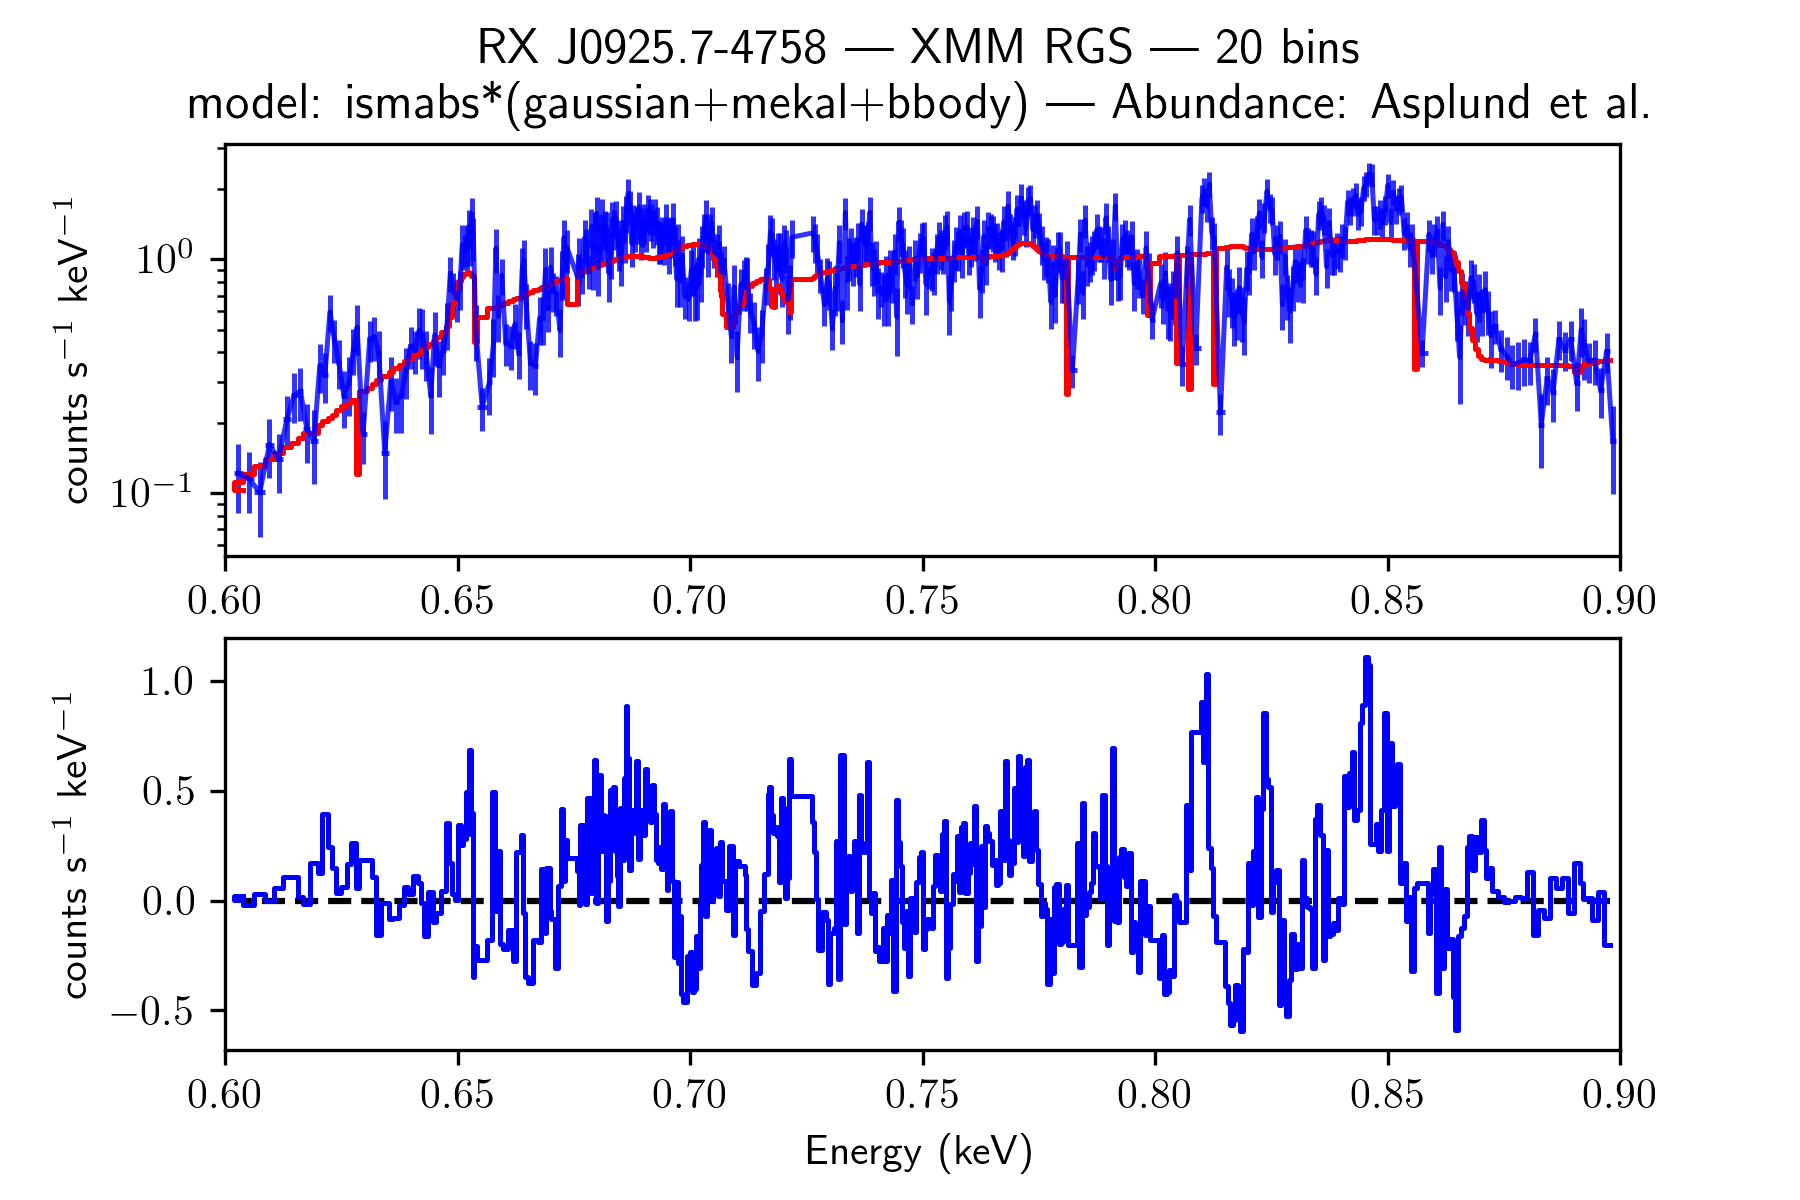
\includegraphics[width=0.9\textwidth]{mrvel-rgs1-o1-m07}} \hfill
				\subfloat[Order 2 \label{xmm:rgs1-m07:o2}]{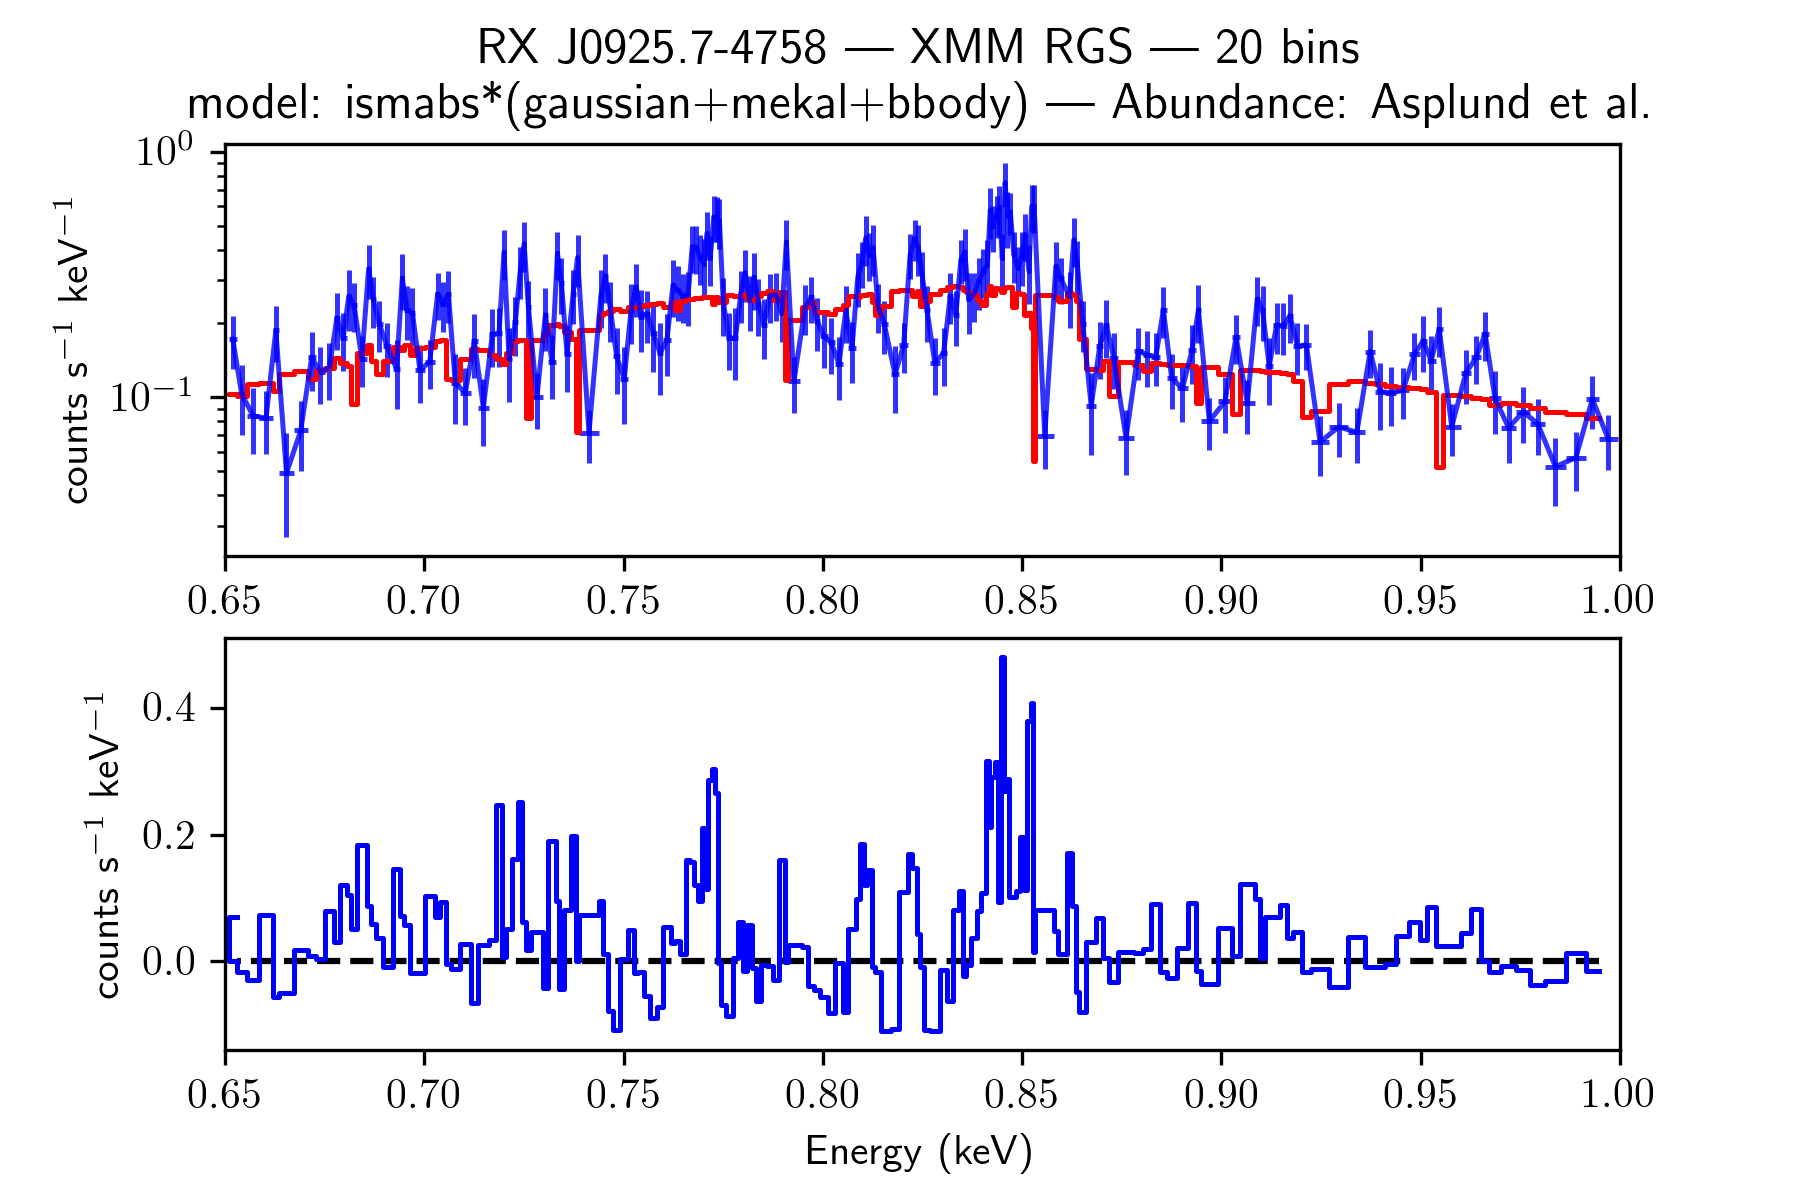
\includegraphics[width=0.9\textwidth]{mrvel-rgs1-o2-m07}} %\hfill
				\caption{Model M07 fit to RGS1 spectra}
				\label{xmm:rgs1-m07}
			\end{figure}
			
			\newpage
			\begin{figure}[h!]
				\centering
				\subfloat[Order 1 \label{xmm:rgs1-m08:o1}]{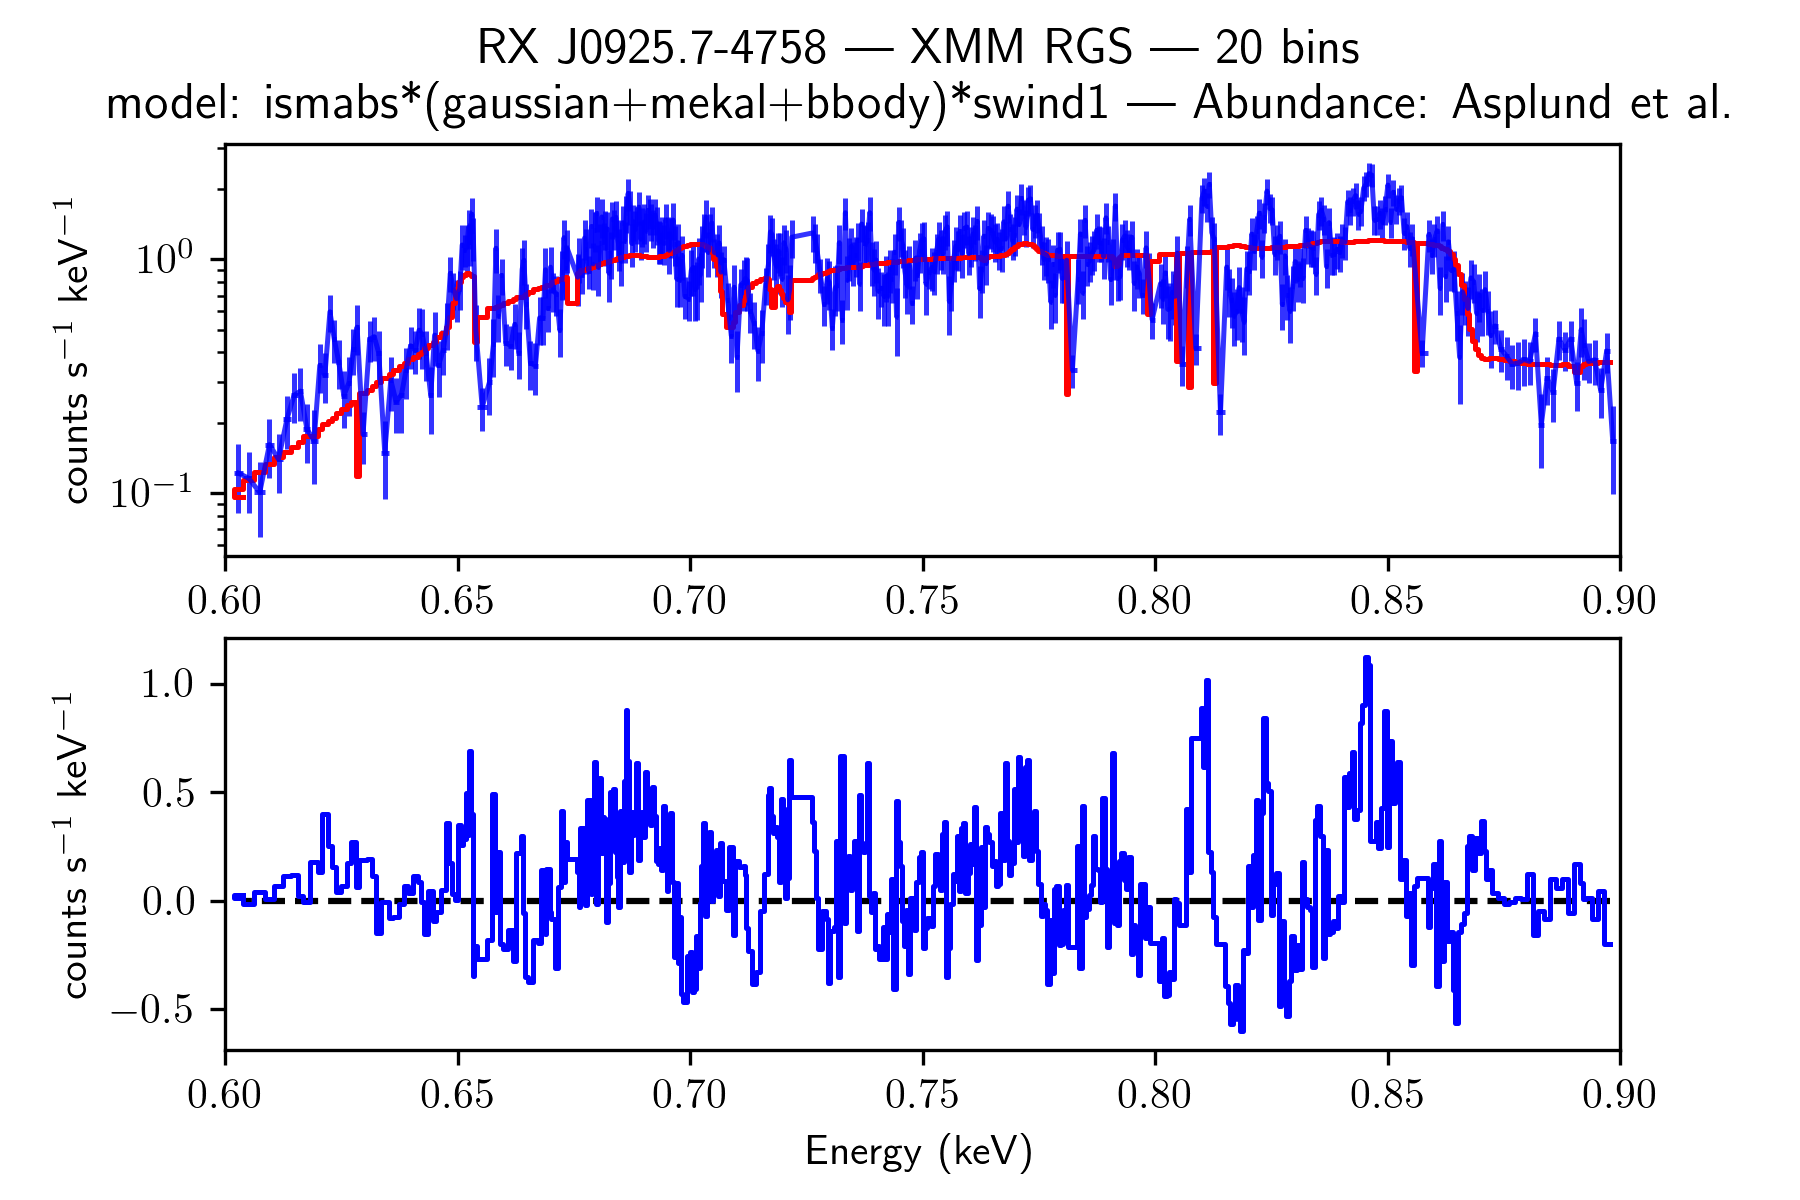
\includegraphics[width=0.9\textwidth]{mrvel-rgs1-o1-m08}} \hfill
				\subfloat[Order 2 \label{xmm:rgs1-m08:o2}]{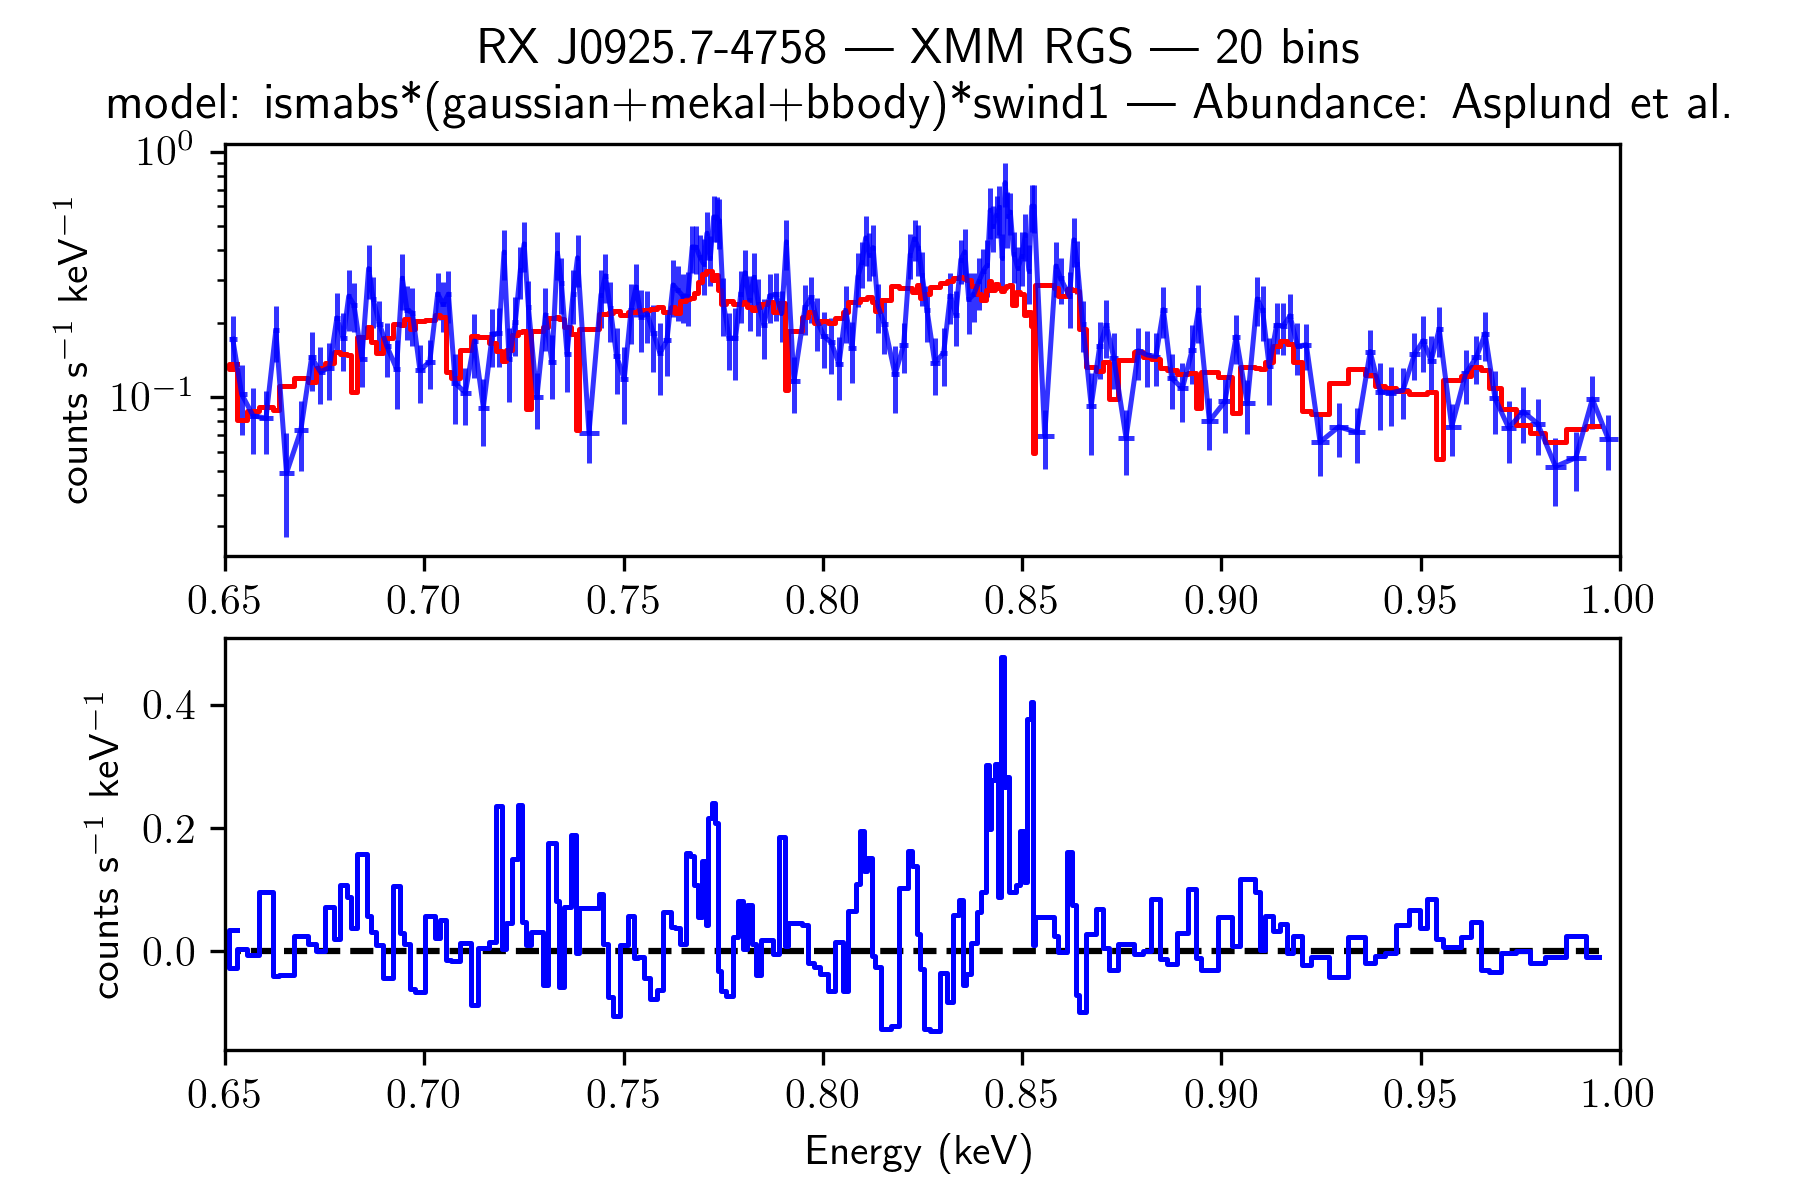
\includegraphics[width=0.9\textwidth]{mrvel-rgs1-o2-m08}} %\hfill
				\caption{Model M08 fit to RGS1 spectra}
				\label{xmm:rgs1-m08}
			\end{figure}
			
			\newpage
			\begin{figure}[h!]
				\centering
				\subfloat[Order 1 \label{xmm:rgs1-m09:o1}]{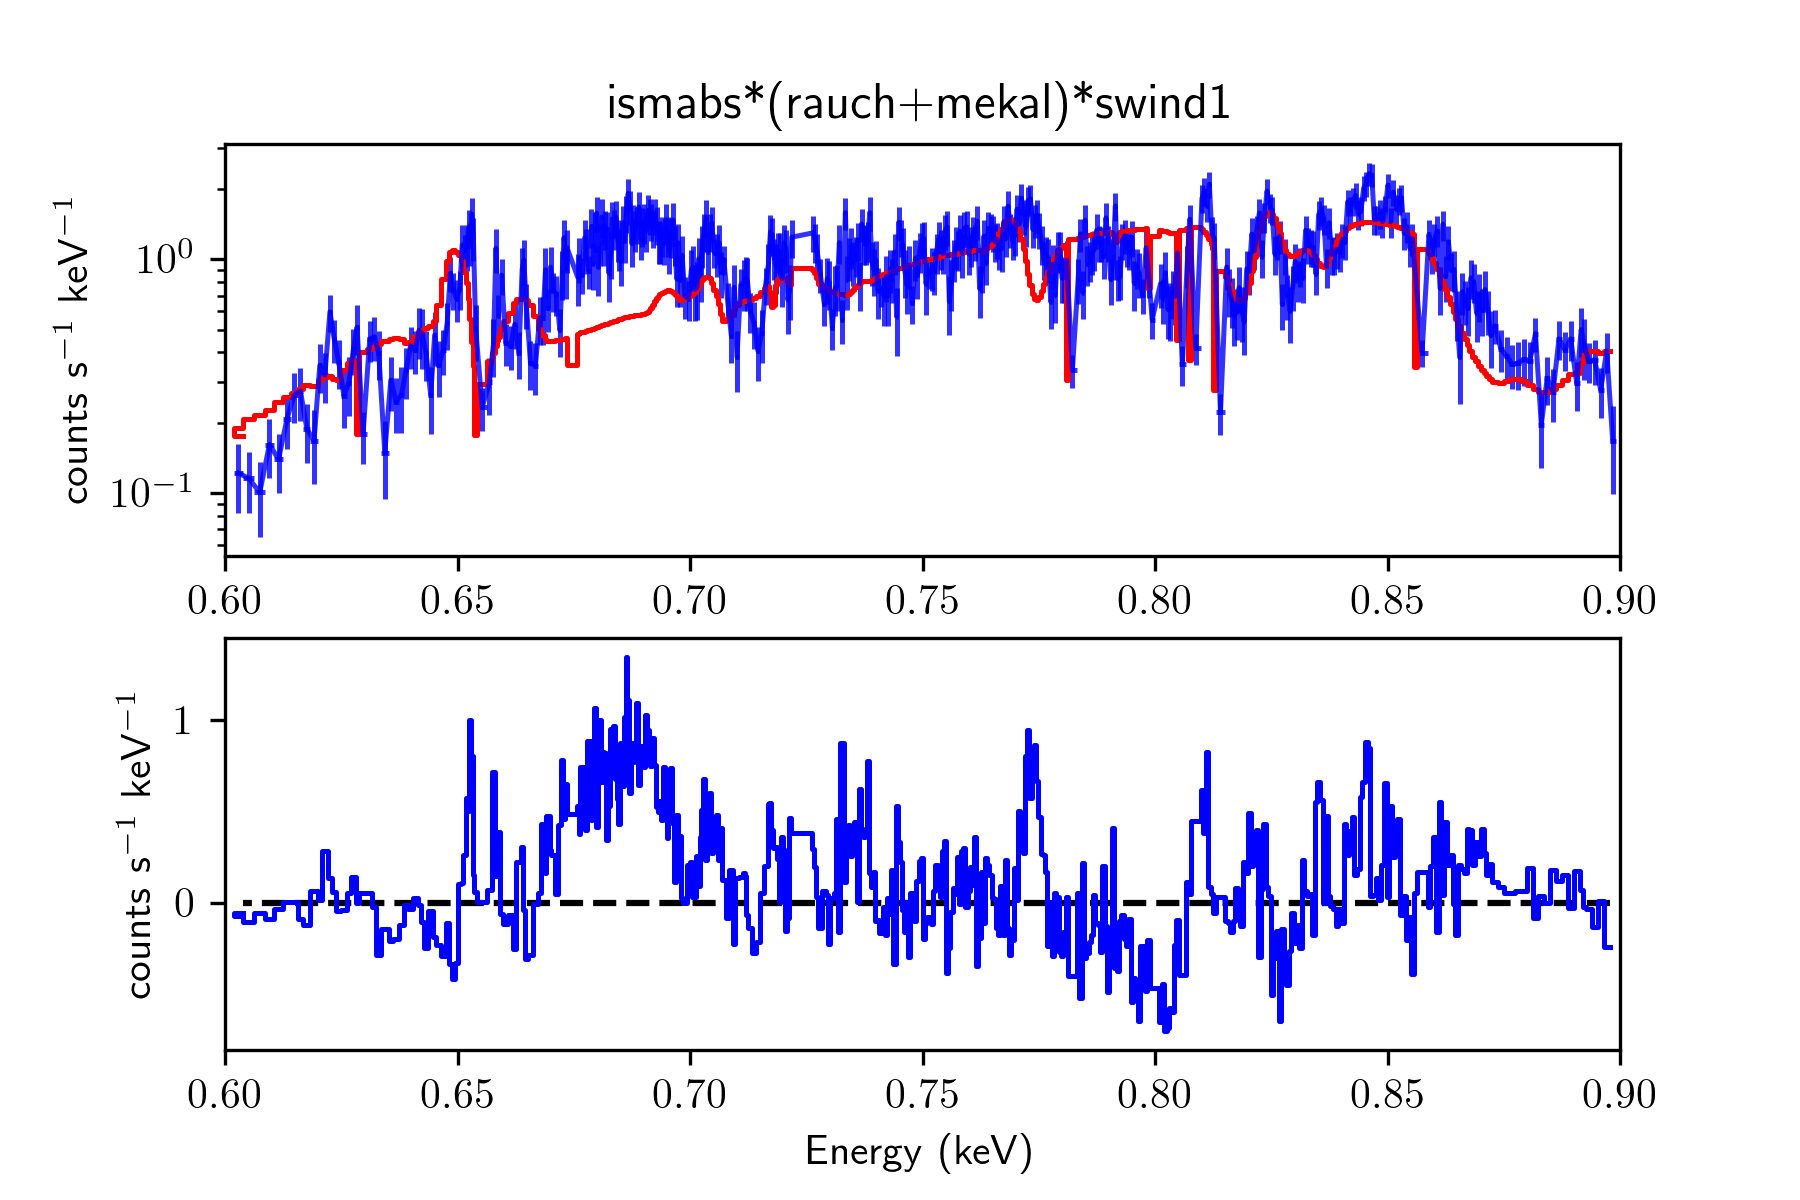
\includegraphics[width=0.9\textwidth]{mrvel-rgs1-o1-m09}} \hfill
				\subfloat[Order 2 \label{xmm:rgs1-m09:o2}]{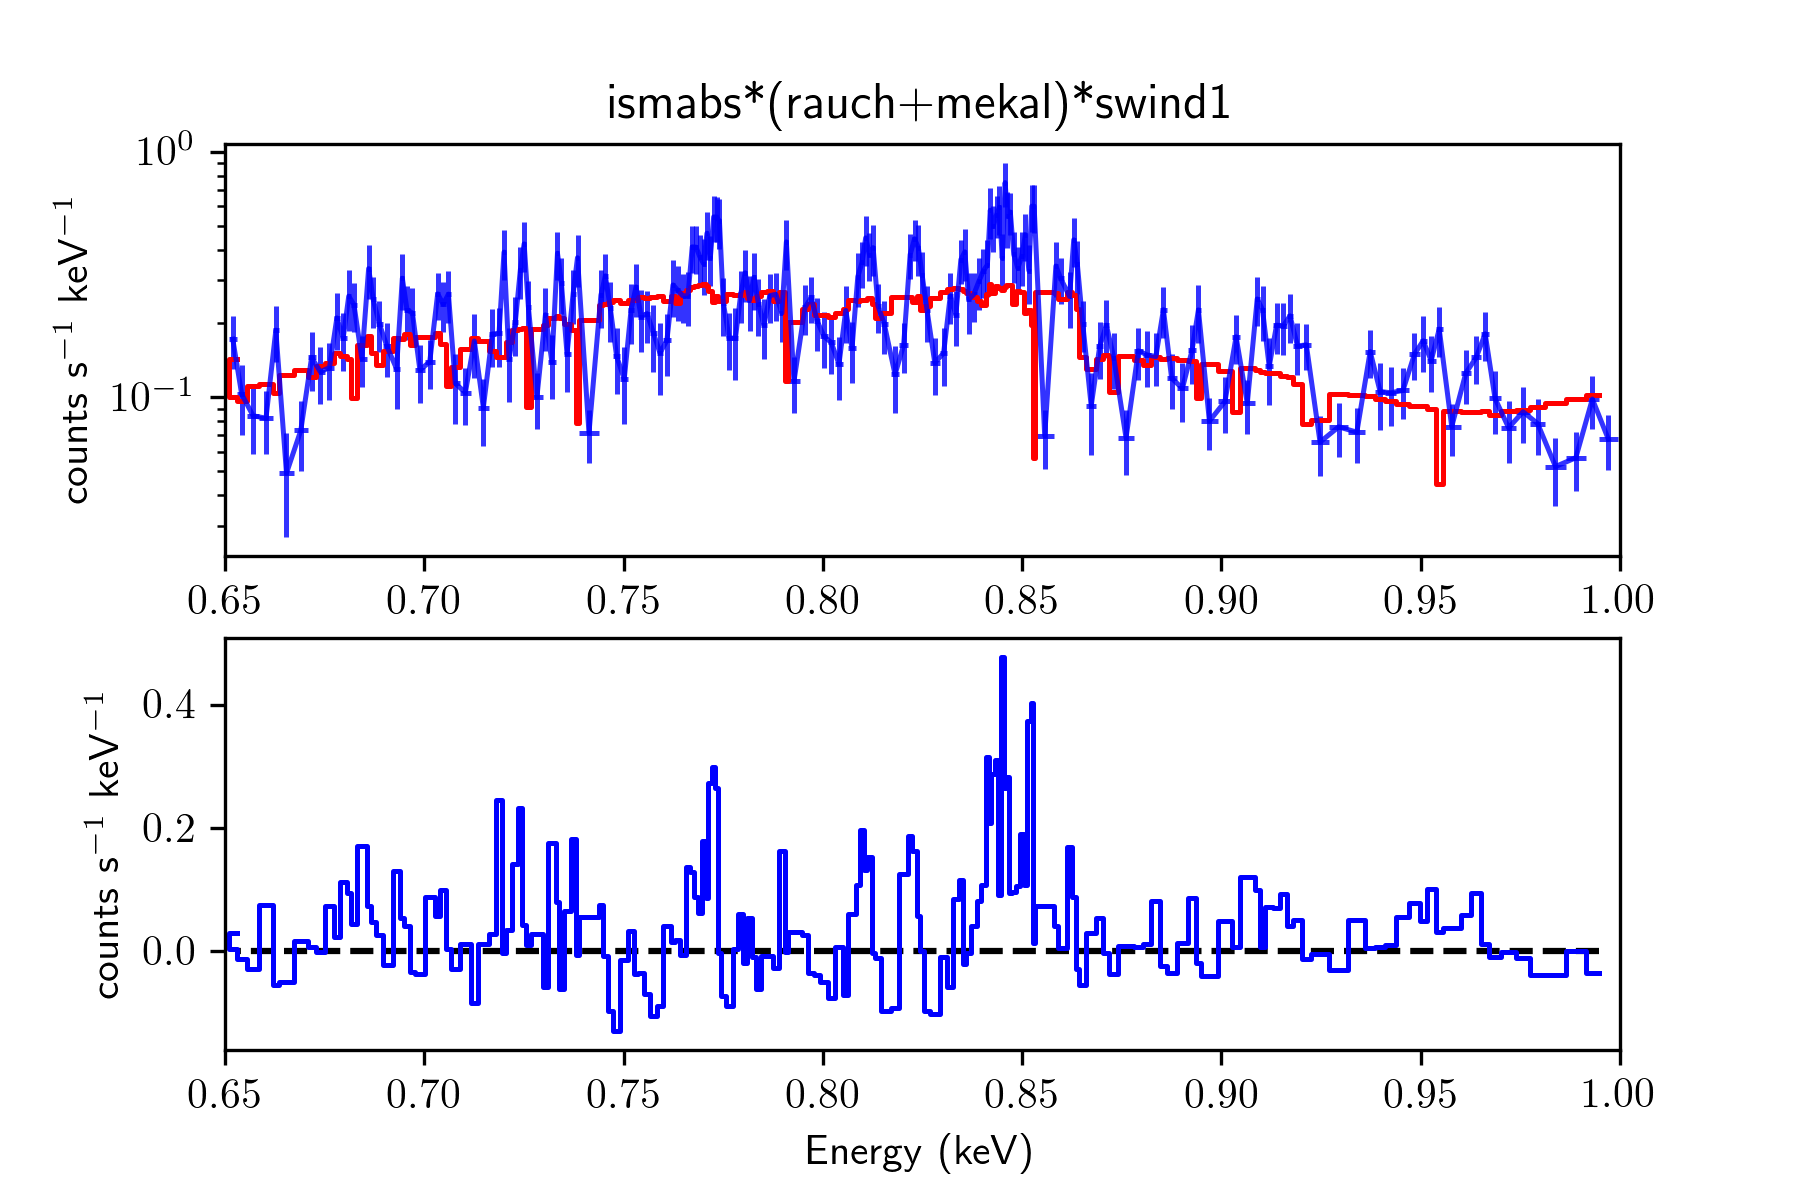
\includegraphics[width=0.9\textwidth]{mrvel-rgs1-o2-m09}} %\hfill
				\caption{Model M09 fit to RGS1 spectra}
				\label{xmm:rgs1-m09}
			\end{figure}
			
			\newpage
			\begin{figure}[h!]
				\centering
				\subfloat[Order 1 \label{xmm:rgs1-m10:o1}]{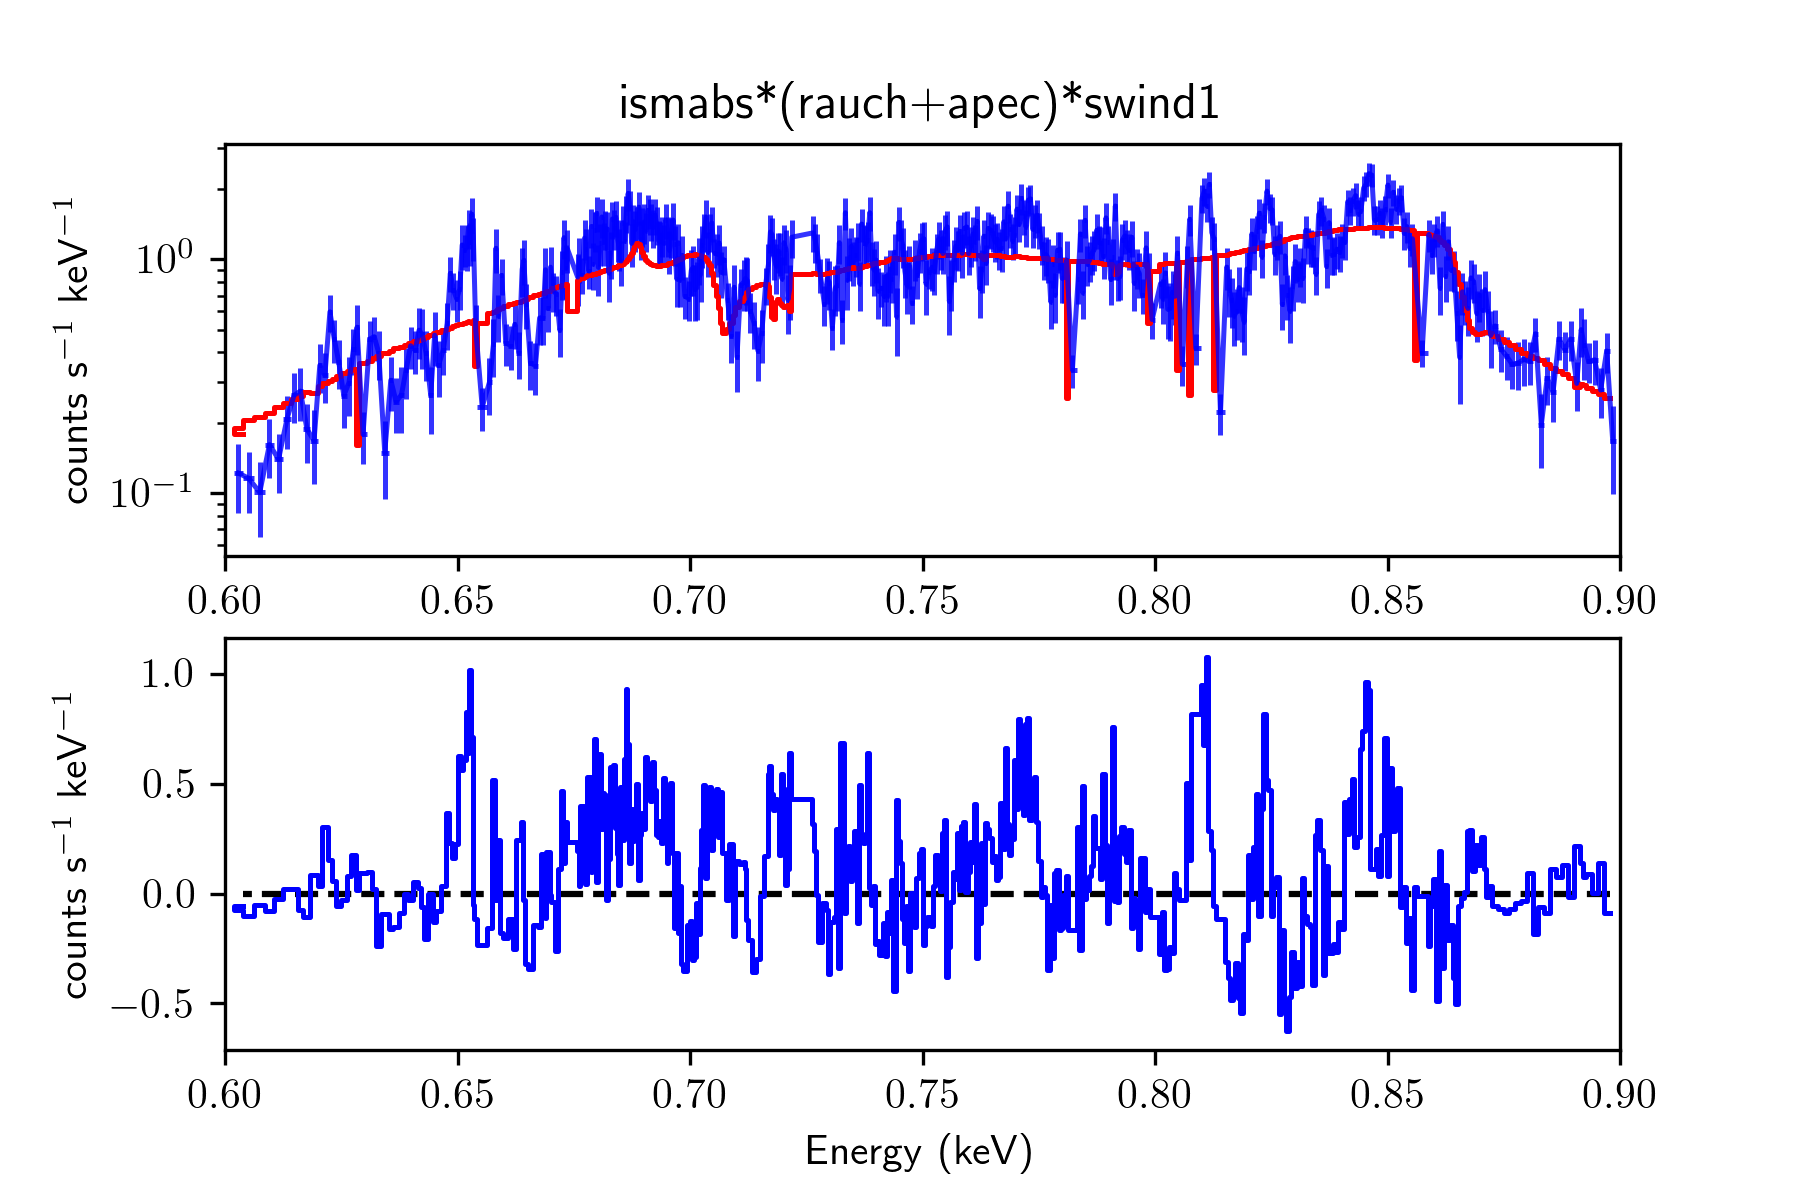
\includegraphics[width=0.9\textwidth]{mrvel-rgs1-o1-m10}} \hfill
				\subfloat[Order 2 \label{xmm:rgs1-m10:o2}]{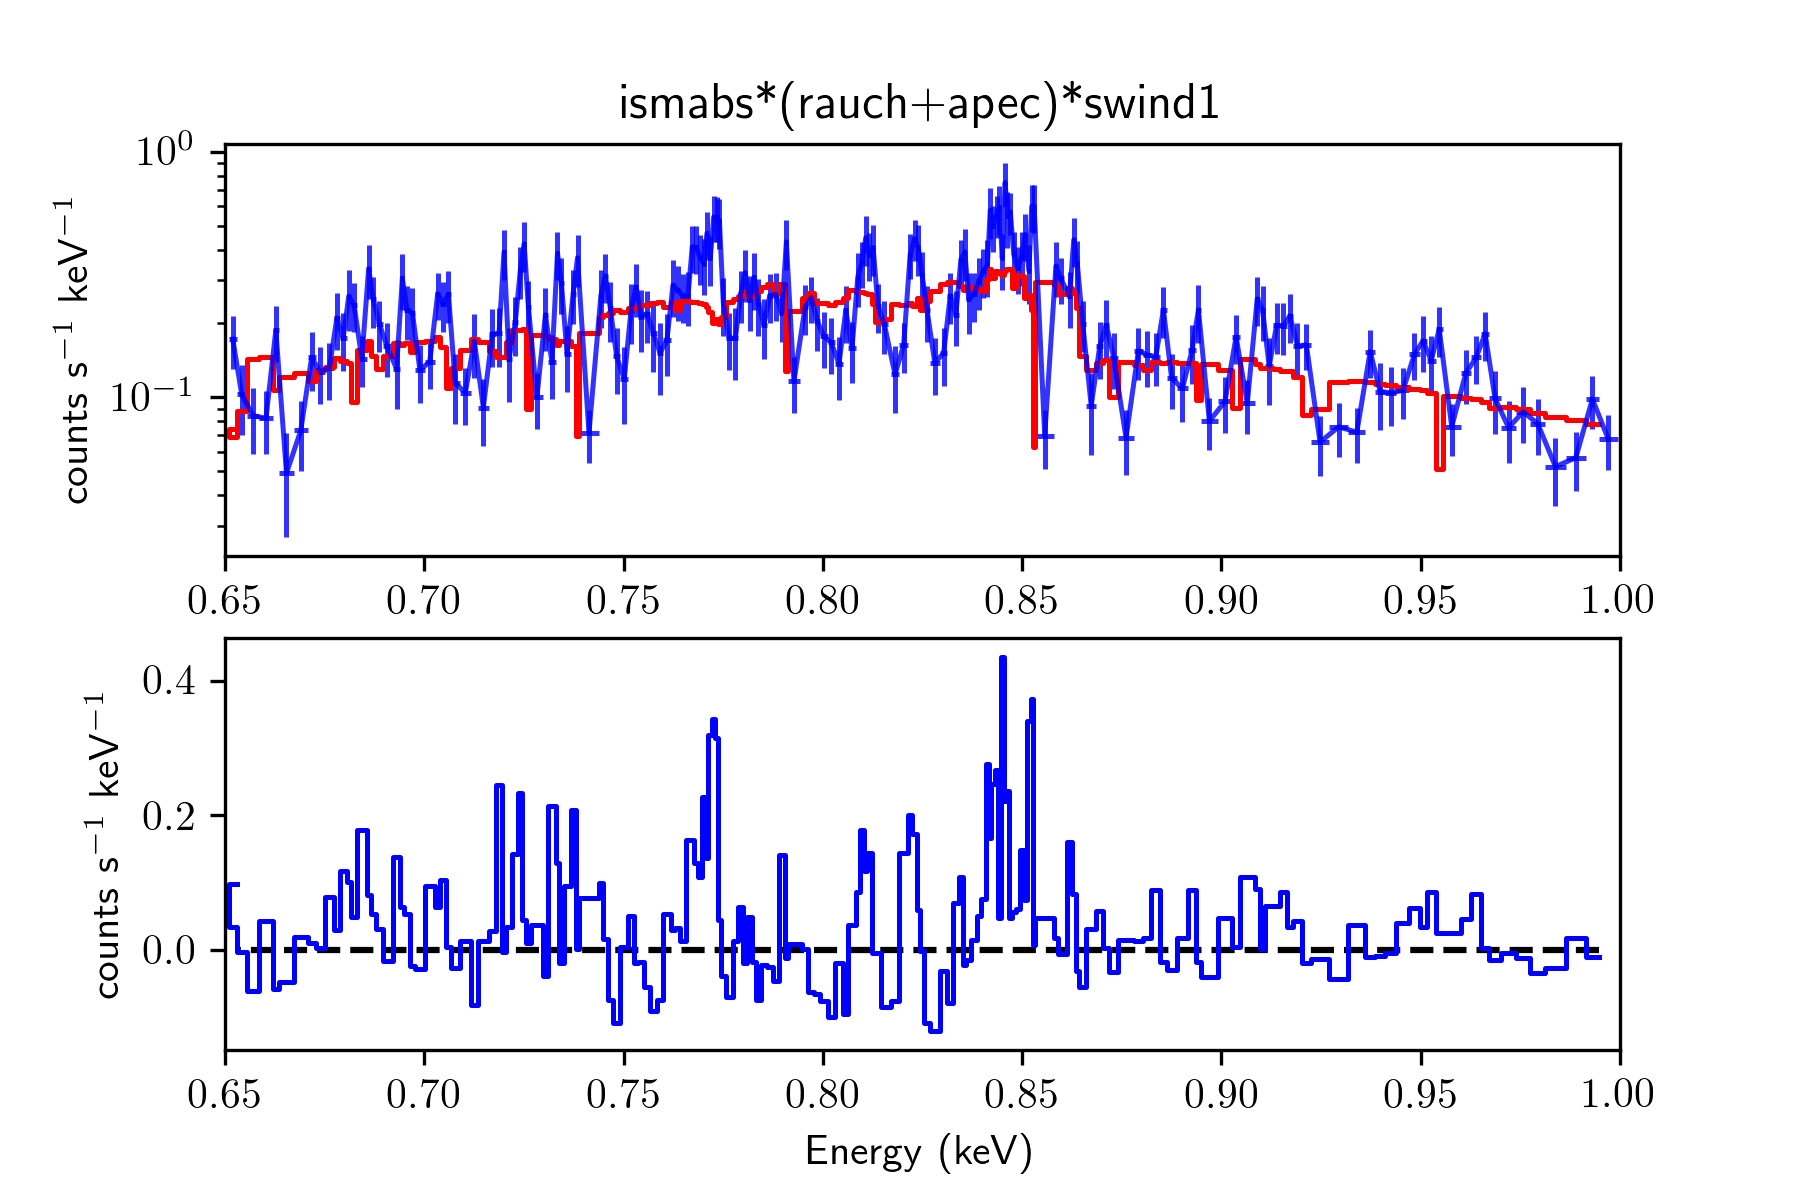
\includegraphics[width=0.9\textwidth]{mrvel-rgs1-o2-m10}} %\hfill
				\caption{Model M10 fit to RGS1 spectra}
				\label{xmm:rgs1-m10}
			\end{figure}
			
			\newpage
			\begin{figure}[h!]
				\centering
				\subfloat[Order 1 \label{xmm:rgs1-m11:o1}]{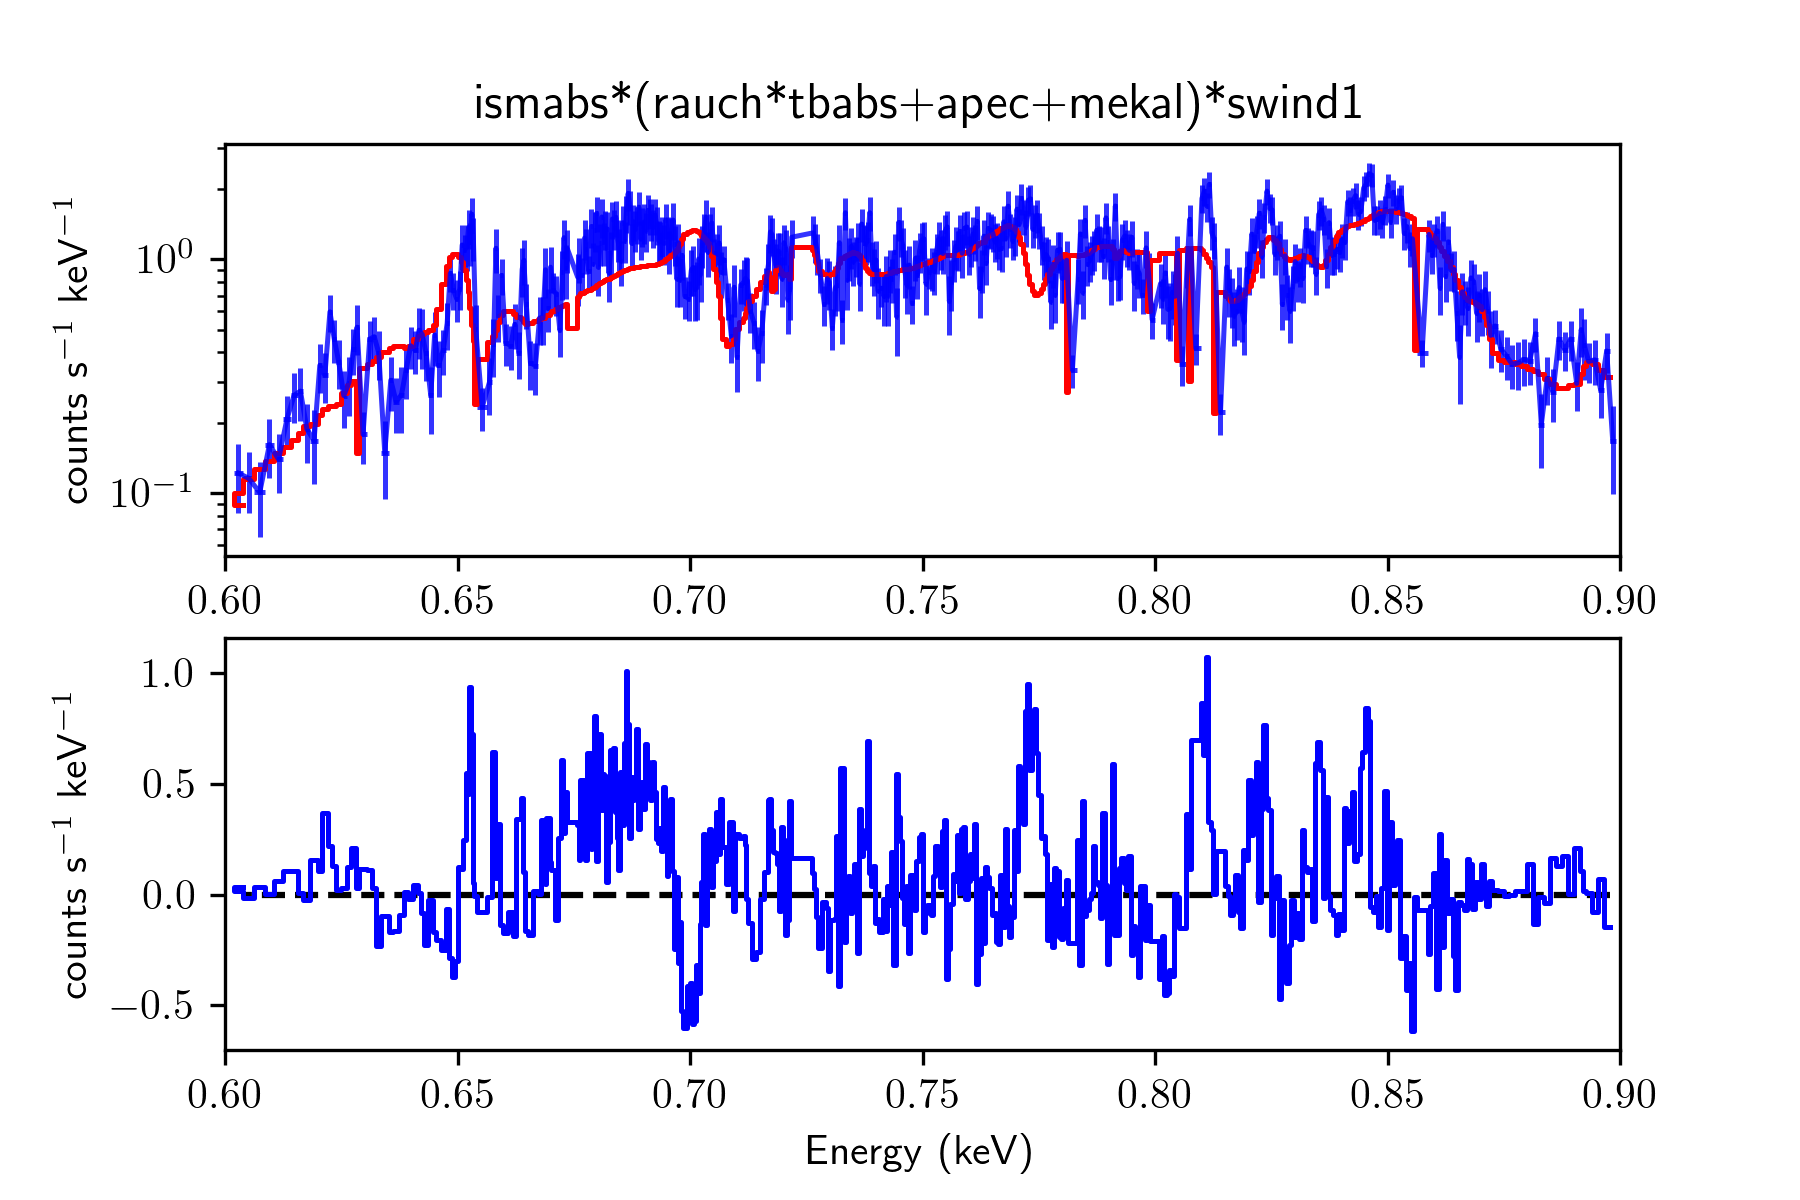
\includegraphics[width=0.9\textwidth]{mrvel-rgs1-o1-m11}} \hfill
				\subfloat[Order 2 \label{xmm:rgs1-m11:o2}]{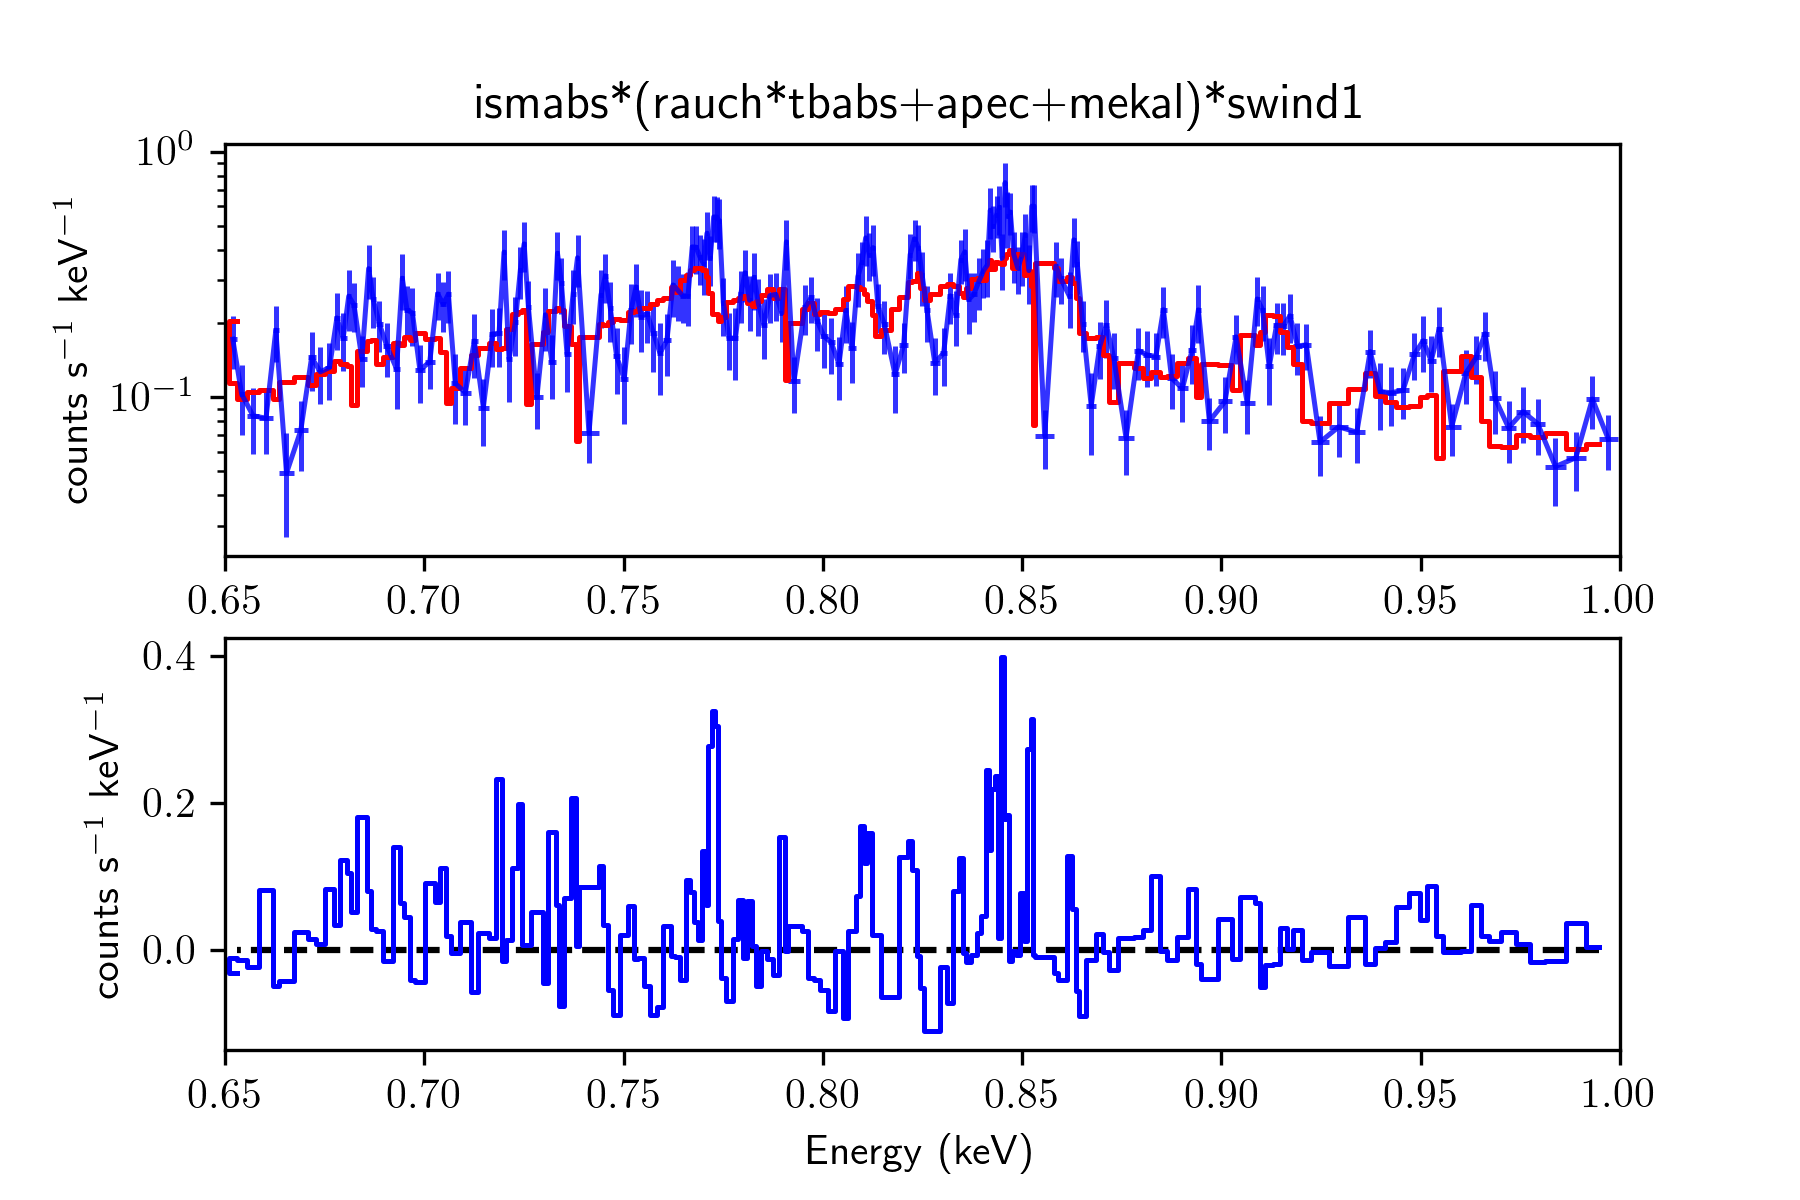
\includegraphics[width=0.9\textwidth]{mrvel-rgs1-o2-m11}} %\hfill
				\caption{Model M11 fit to RGS1 spectra}
				\label{xmm:rgs1-m11}
			\end{figure}
			
			\newpage
			\begin{figure}[h!]
				\centering
				\subfloat[Order 1 \label{xmm:rgs1-m12:o1}]{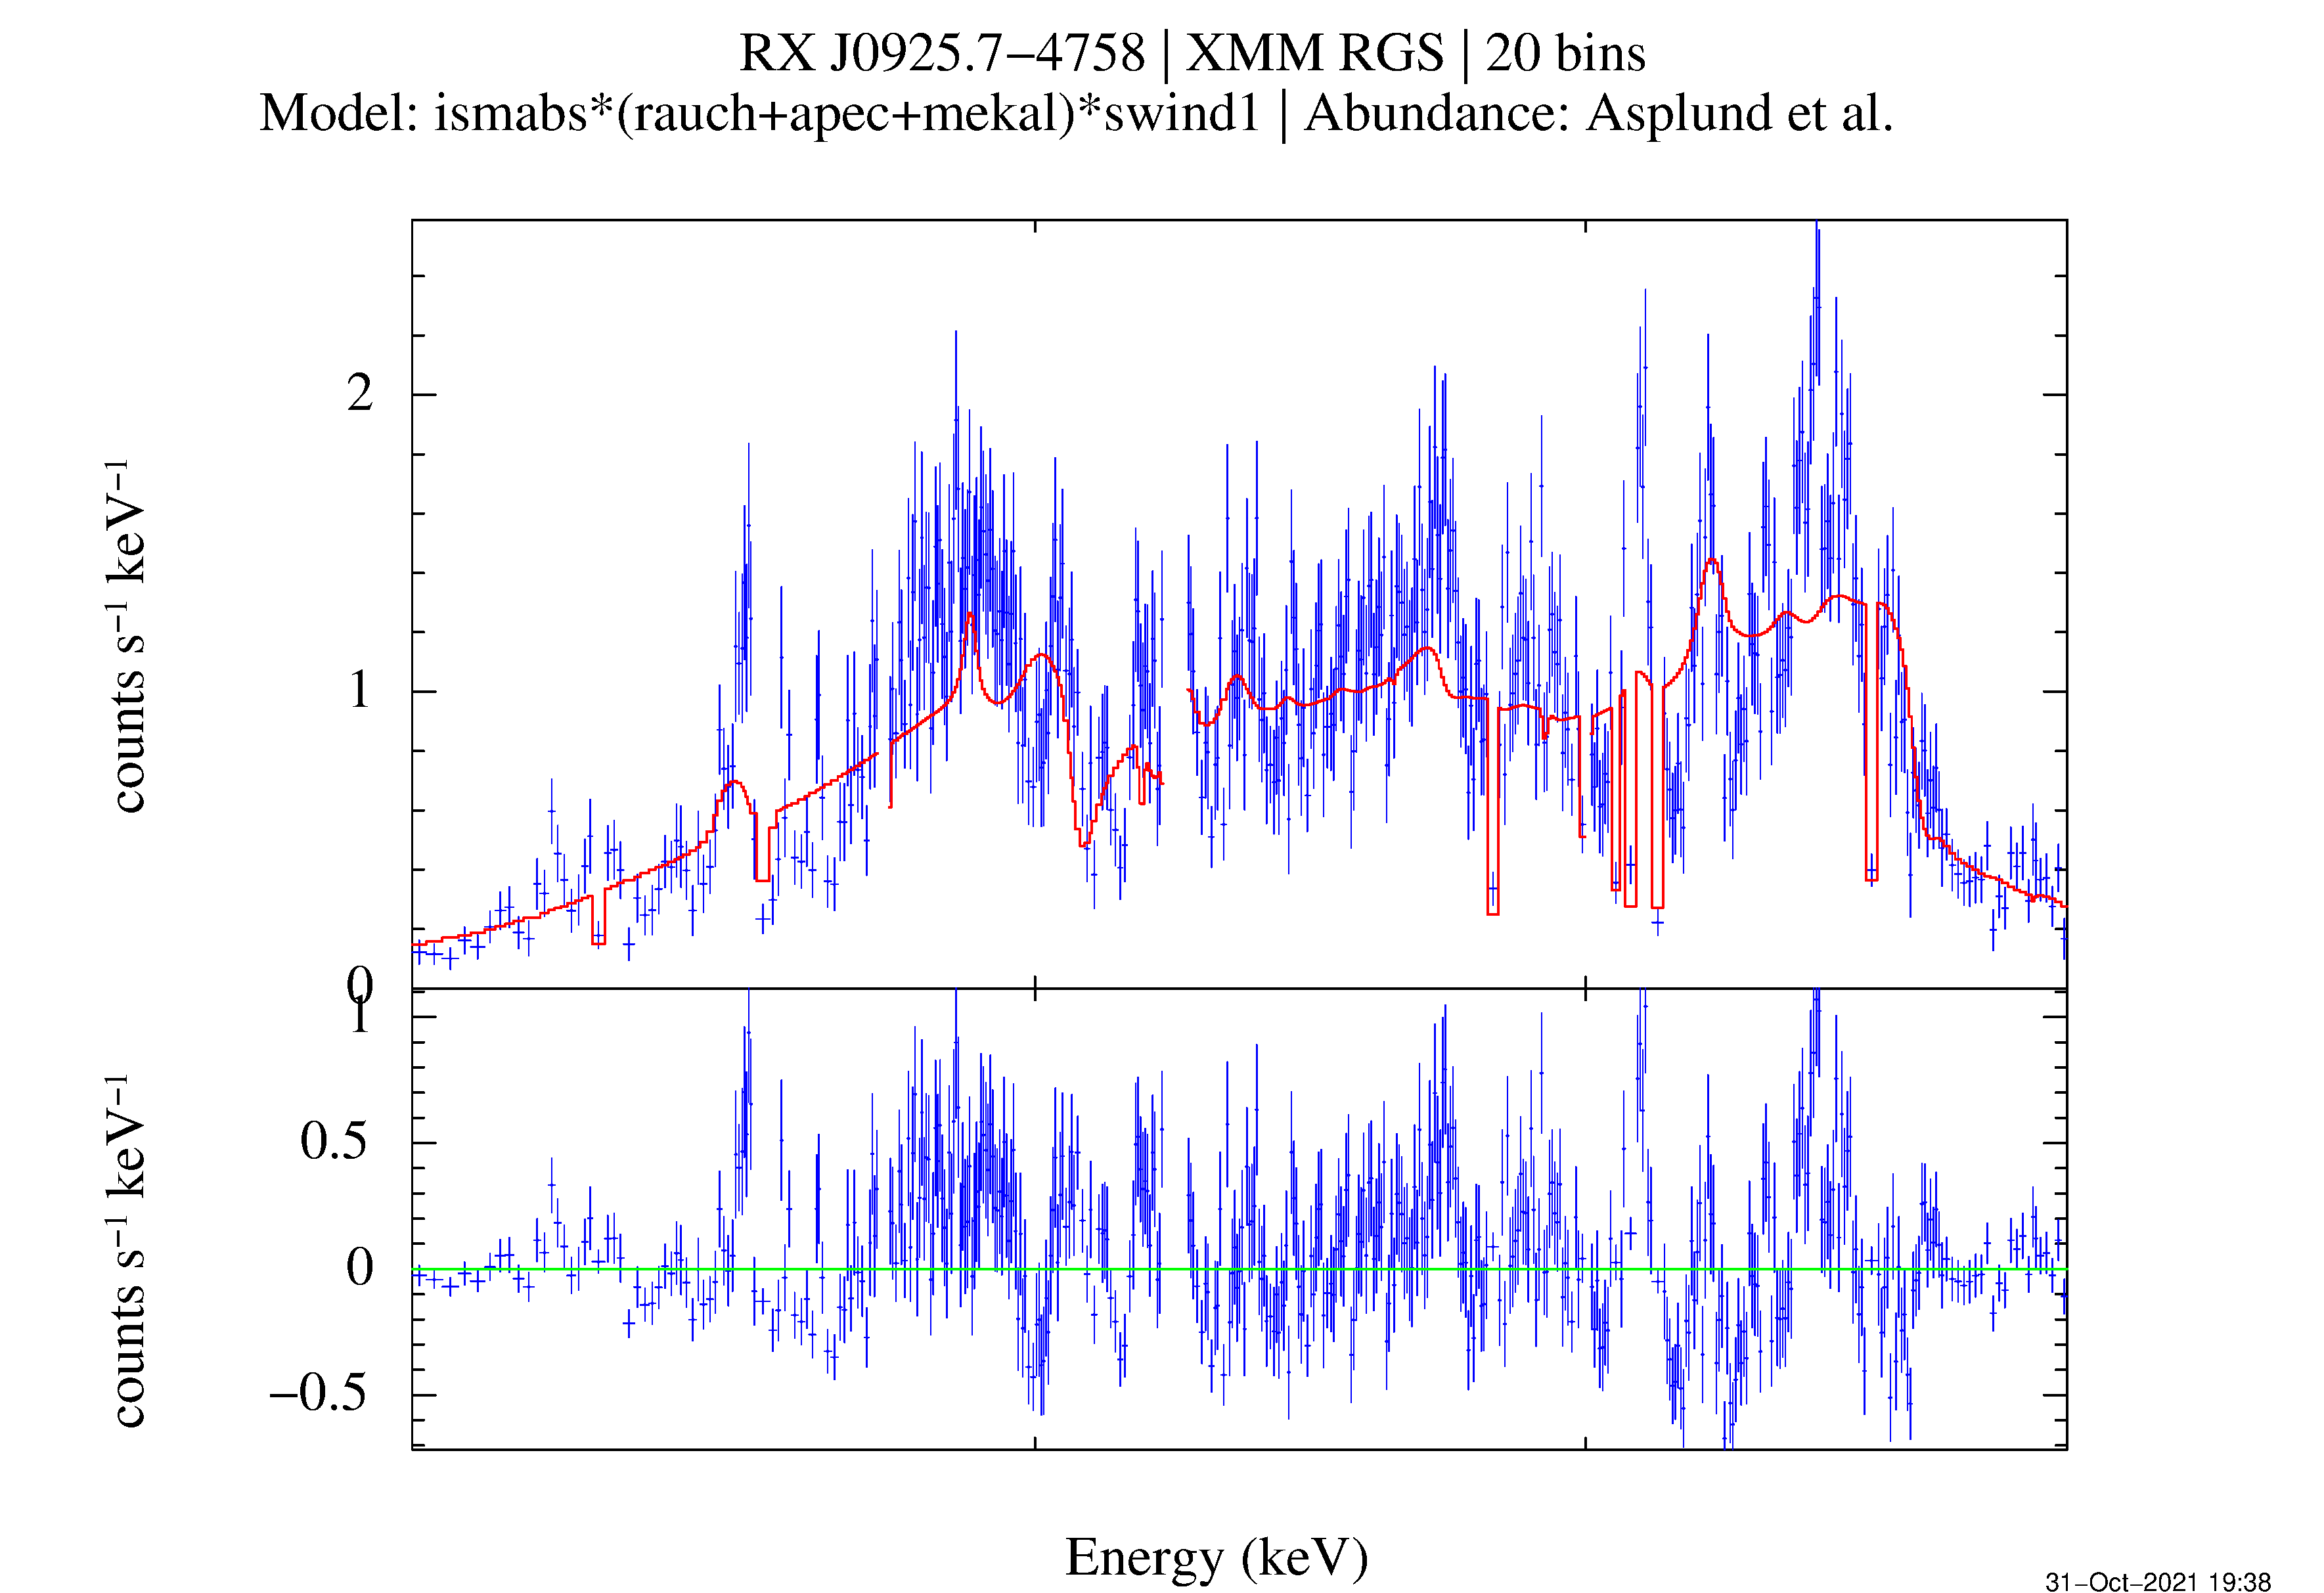
\includegraphics[width=0.9\textwidth]{mrvel-rgs1-o1-m12}} \hfill
				\subfloat[Order 2 \label{xmm:rgs1-m12:o2}]{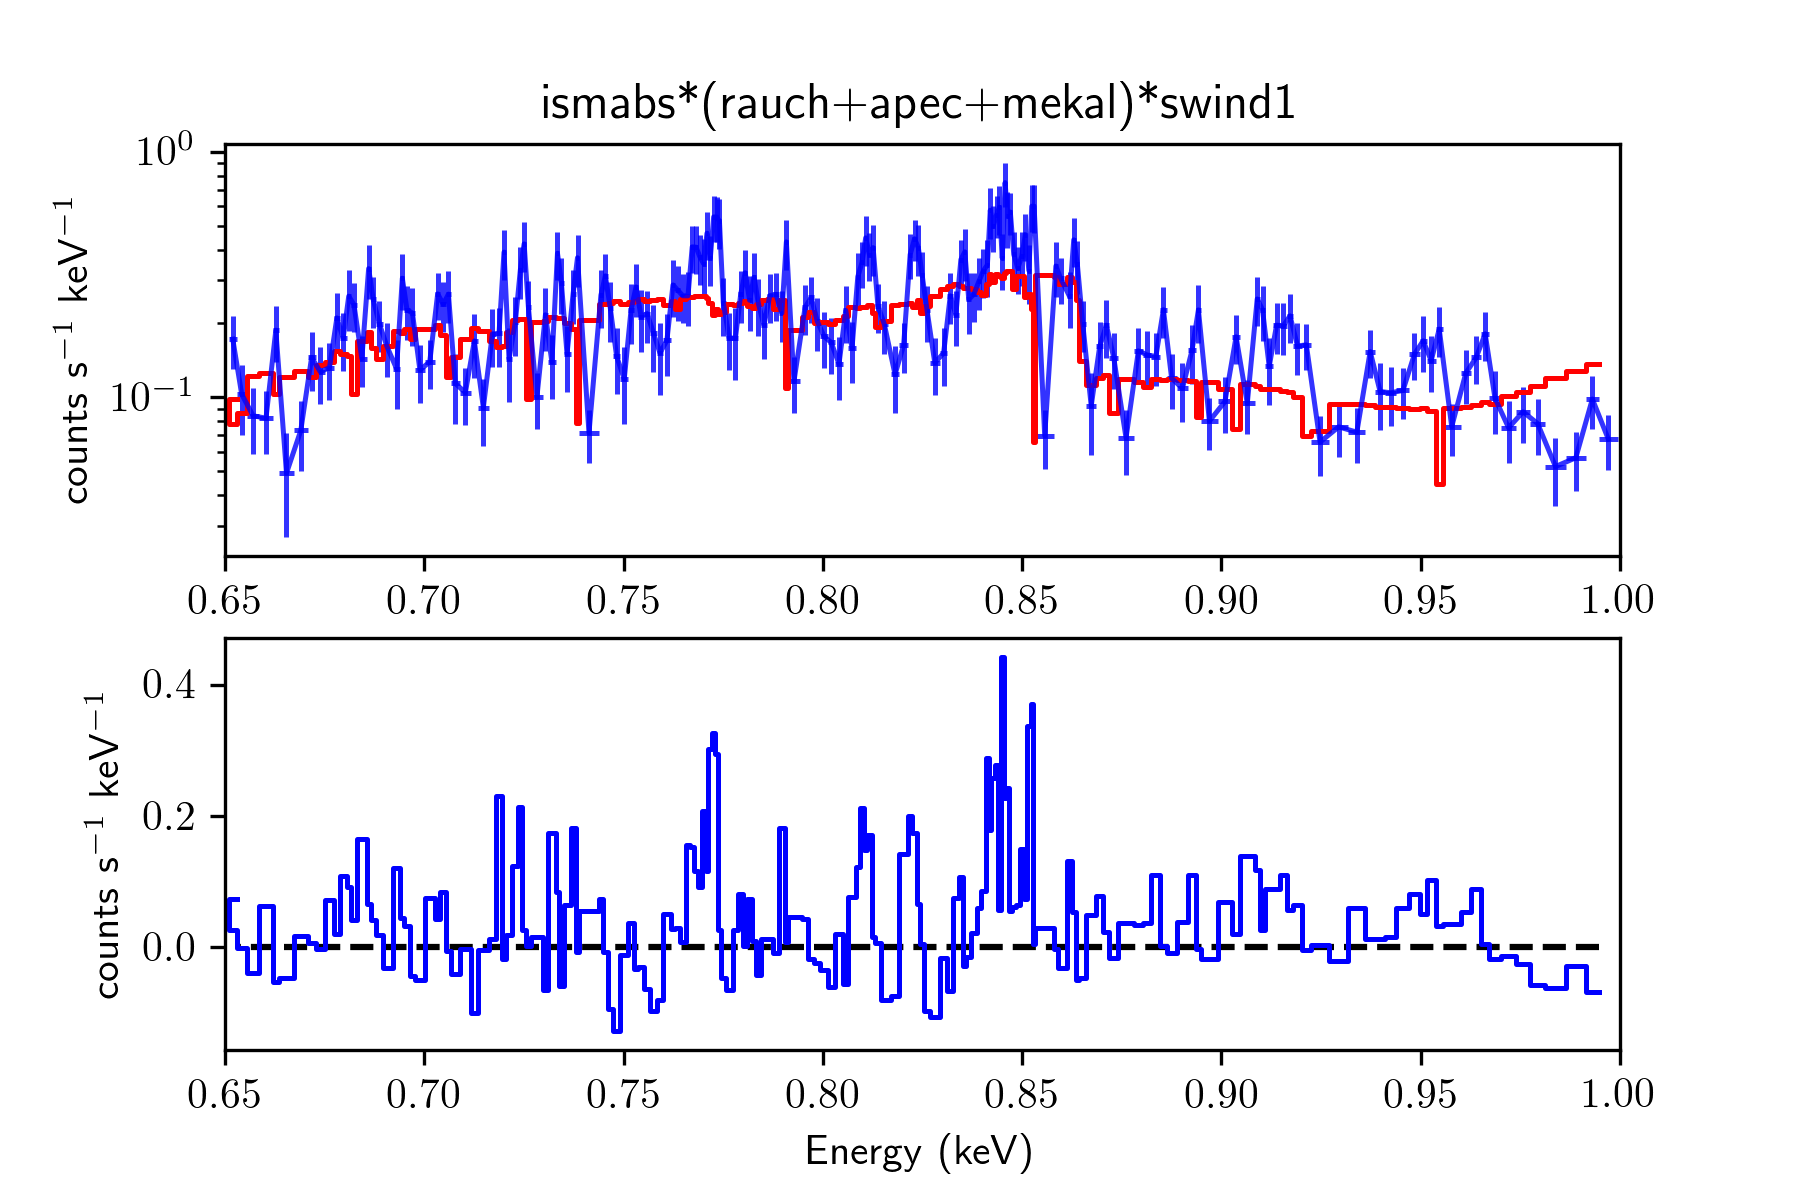
\includegraphics[width=0.9\textwidth]{mrvel-rgs1-o2-m12}} %\hfill
				\caption{Model M12 fit to RGS1 spectra}
				\label{xmm:rgs1-m12}
			\end{figure}
		
		%\newpage
		\subsection{Fitting of RGS2 Spectra} \label{hi-resolution:analysis:rgs2}
		
			\begin{figure}[h!]
				\centering
				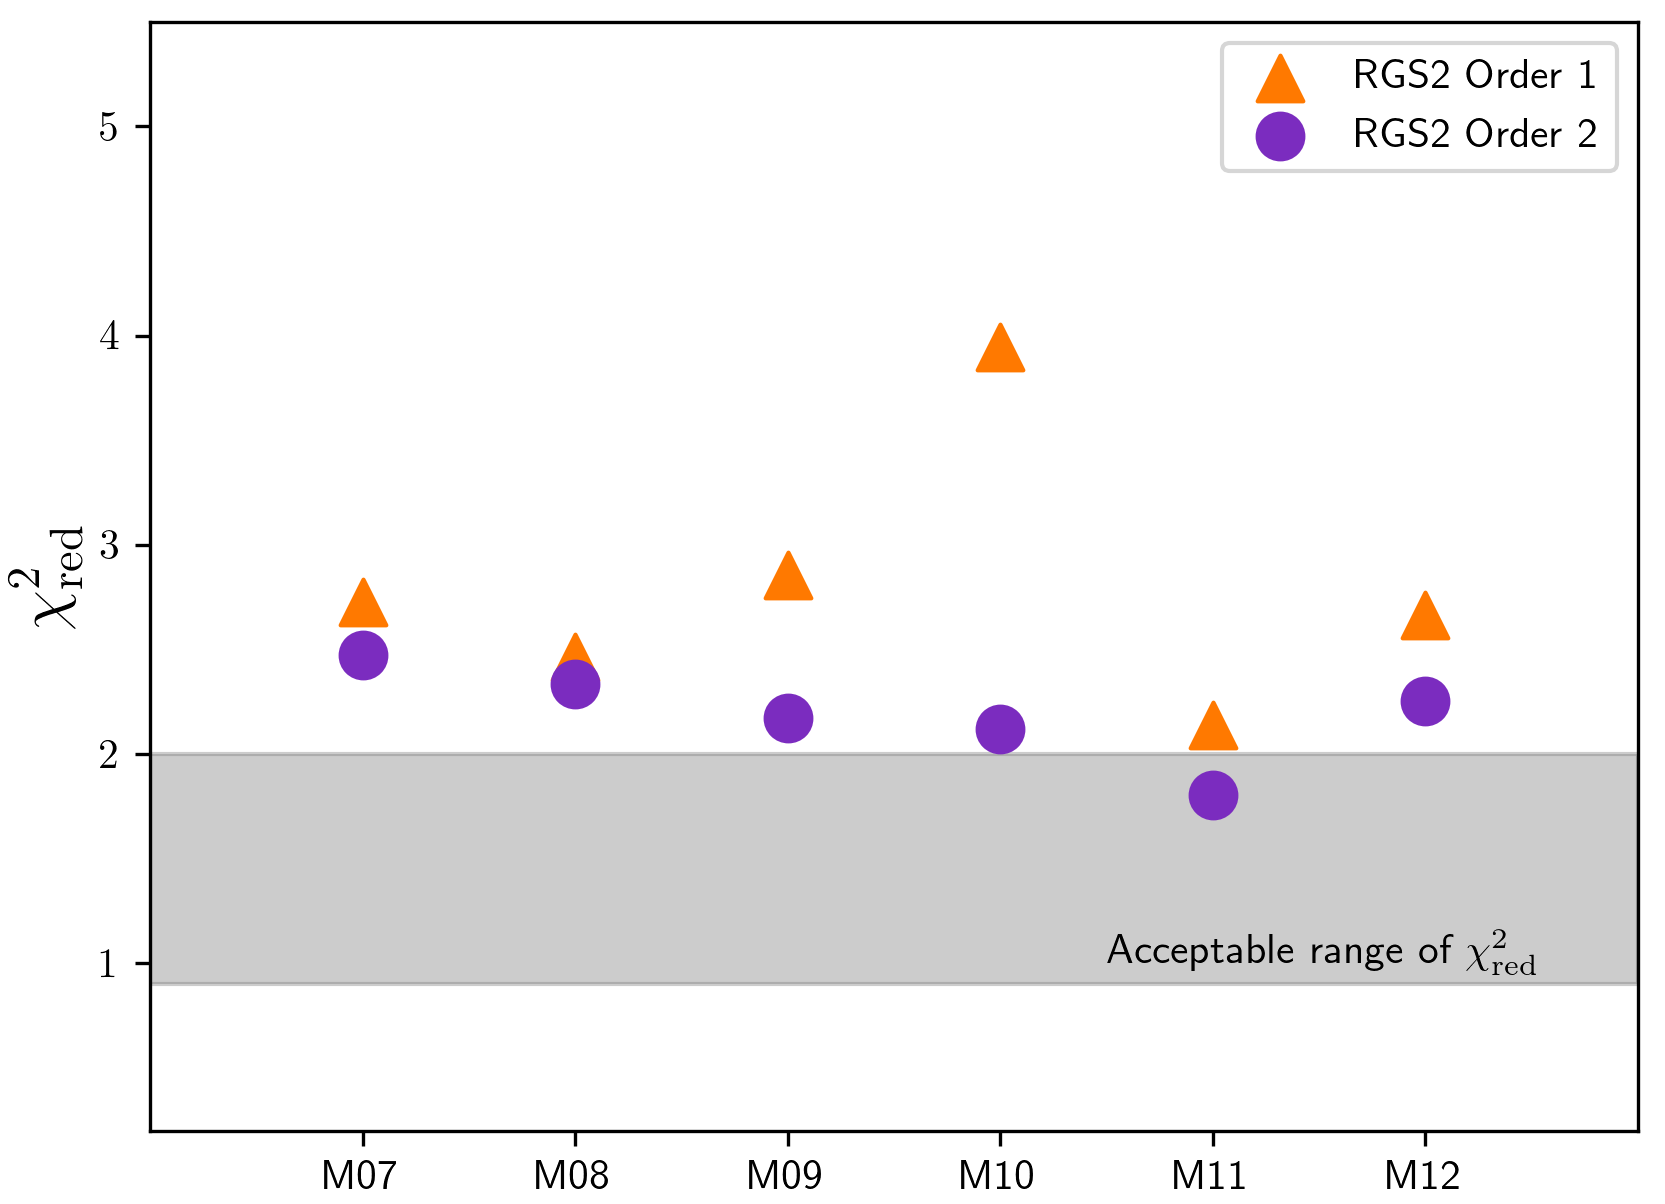
\includegraphics[width=\textwidth]{mrvel-rgs2-chisq_new}
				\caption{$\chi^2_\text{red}$ trend of RGS2 spectra from RX J0925.7-4758}
				\label{fig:mrvel-rgs2-chisq}
			\end{figure}
			
			We present here the results of fitting a selection of spectral models to the RGS2 data from RX J0925.7-4758. We assess the quality of each fit using the values of the reduced chi-squared statistic ($\chi^2_\text{reduced}$). Acceptable models typically have $\chi^2_\text{reduced}$ values in the range of 1 to 2. The fitting statistics are summarized in table \ref{tab:fit-stat:rgs1}.  These values are also plotted in figure \ref{fig:mrvel-rgs1-chisq} to visually identify models with acceptable $\chi^2_\text{reduced}$ values.
			%Here as well the best fits for both diffraction orders were obtained using the model M11. This seems to suggest that model M11 might be the best candidate model for RX J0925.7-4758. All the other models yield $\chi^2_\text{red}$ to be outside the acceptable range, with the exception of the model M08, which lies almost on the borderline. The trend shown by the $\chi^2_\text{red}$ across all the models considered here are shown in figure \ref{fig:mrvel-rgs2-chisq}.
			\begin{table}[!htb]
				\centering
				\caption{Fitting statistics of RGS2 spectra from RX J0925.7-4758}
				\label{tab:fit-stat:rgs2}
				\begin{tabular}{c|cc|cc}
					\hline
					\multirow{2}{*}{\textbf{Model ID}} & \multicolumn{2}{c|}{\textbf{RGS 1 $\vert$ Order 1}} & \multicolumn{2}{c}{\textbf{RGS 1 $\vert$ Order 2}} \\ \cline{2-5} & {$\boldsymbol{\chi^2}$/\textbf{d.o.f}} & {$\boldsymbol{\chi^2_\text{reduced}}$} & {$\boldsymbol{\chi^2}$/\textbf{d.o.f}} & {$\boldsymbol{\chi^2_\text{reduced}}$} \\ \hline
					{M07} & {1506.9/553} & {2.73} & {497.3/201} & {2.47} \\
					{M08} & {1353.8/550} & {2.46} & {462.0/198} & {2.33} \\
					{M09} & {1576.8/552} & {2.86} & {434.6/200} & {2.17} \\
					{M10} & {2176.7/552} & {3.94} & {423.8/200} & {2.12} \\
					{M11} & {1173.8/549} & {2.14} & {355.2/197} & {1.80} \\
					{M12} & {1465.1/552} & {2.65} & {445.9/198} & {2.25} \\ \hline
				\end{tabular}
			\end{table}
			
			As evident from table \ref{tab:fit-stat:rgs2} or figure \ref{fig:mrvel-rgs2-chisq}, the model M11 again provides the best fit for both spectral orders. While other models do not yield the best fit according to the $\chi^2_\text{reduced}$ statistic, with the exception of the models M09 and M10, which lies almost on the borderline for order 2 spectra. They still provide a reasonable fit that surpasses those found in previous literature. This trend of $\chi^2_\text{reduced}$ across all the models is illustrated in figure \ref{fig:mrvel-rgs2-chisq}.
			
			\subsubsection*{Detailed spectral fits}
				The accompanying figures illustrate the fitted spectra and their corresponding residuals for each model applied to RGS2 data. These visual representations provide a valuable tool for evaluating the quality of our spectral fits. By comparing the fitted spectra to the observed data, we can assess how well each model captures the underlying spectral features and intensity variations. Furthermore, the residuals, which represent the difference between the observed and fitted spectra, offer insights into the model's accuracy. A well-fitting model should produce residuals that are randomly distributed around zero, indicating a minimal discrepancy between the model predictions and the observed data. Conversely, systematic deviations in the residuals may suggest that the model is incomplete or that there are underlying systematic errors in the data. By carefully analyzing these figures, we can identify potential shortcomings in our models and refine our understanding of the physical processes governing the observed celestial object.
				%The following set of figures present the fitted spectra along with their residuals for each model applied to RGS2 data. These figures allow for a visual inspection of the quality of the fit for each model.
			%The fitted spectra, along with the residuals are displayed as follows:
			\newpage
			\begin{figure}[h!]
				\centering
				\subfloat[Order 1 \label{xmm:rgs2-m07:o1}]{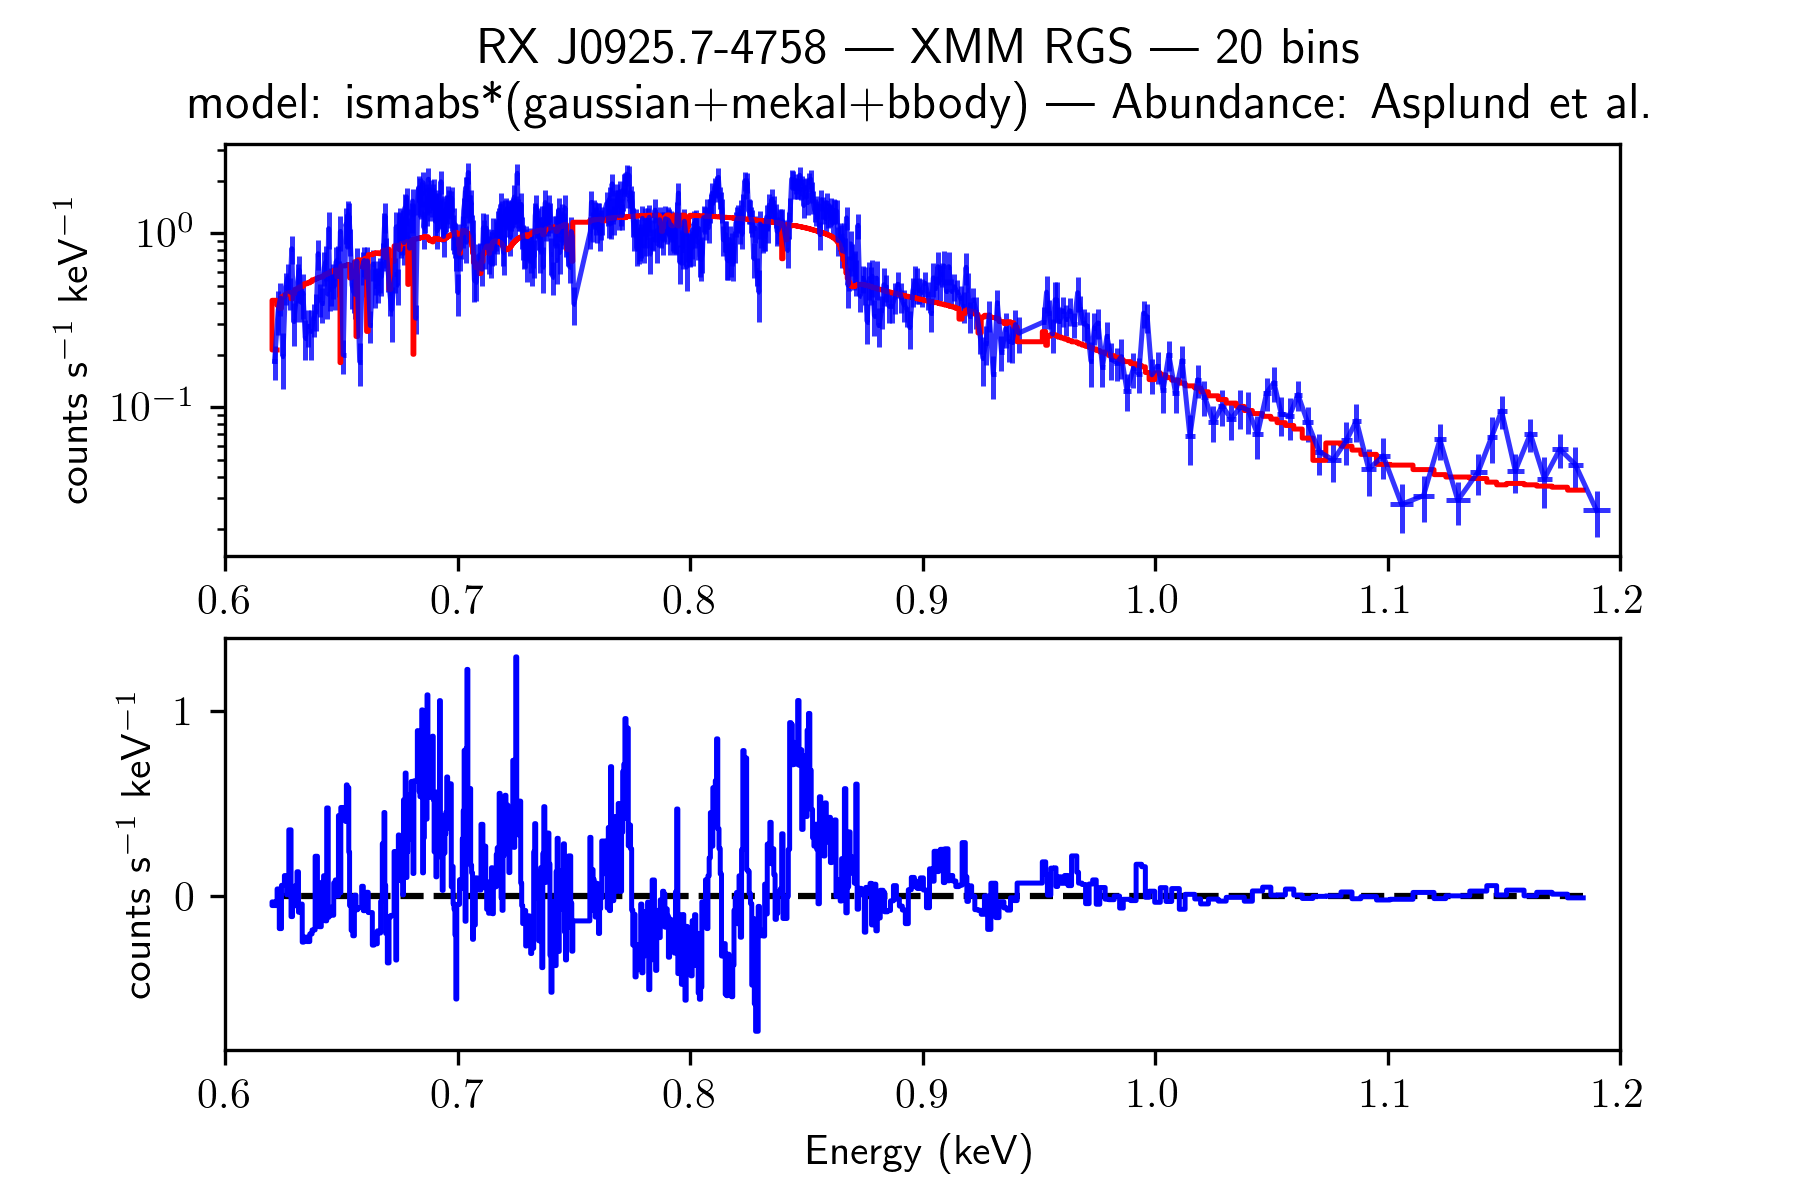
\includegraphics[width=0.9\textwidth]{mrvel-rgs2-o1-m07}} \hfill
				\subfloat[Order 2 \label{xmm:rgs2-m07:o2}]{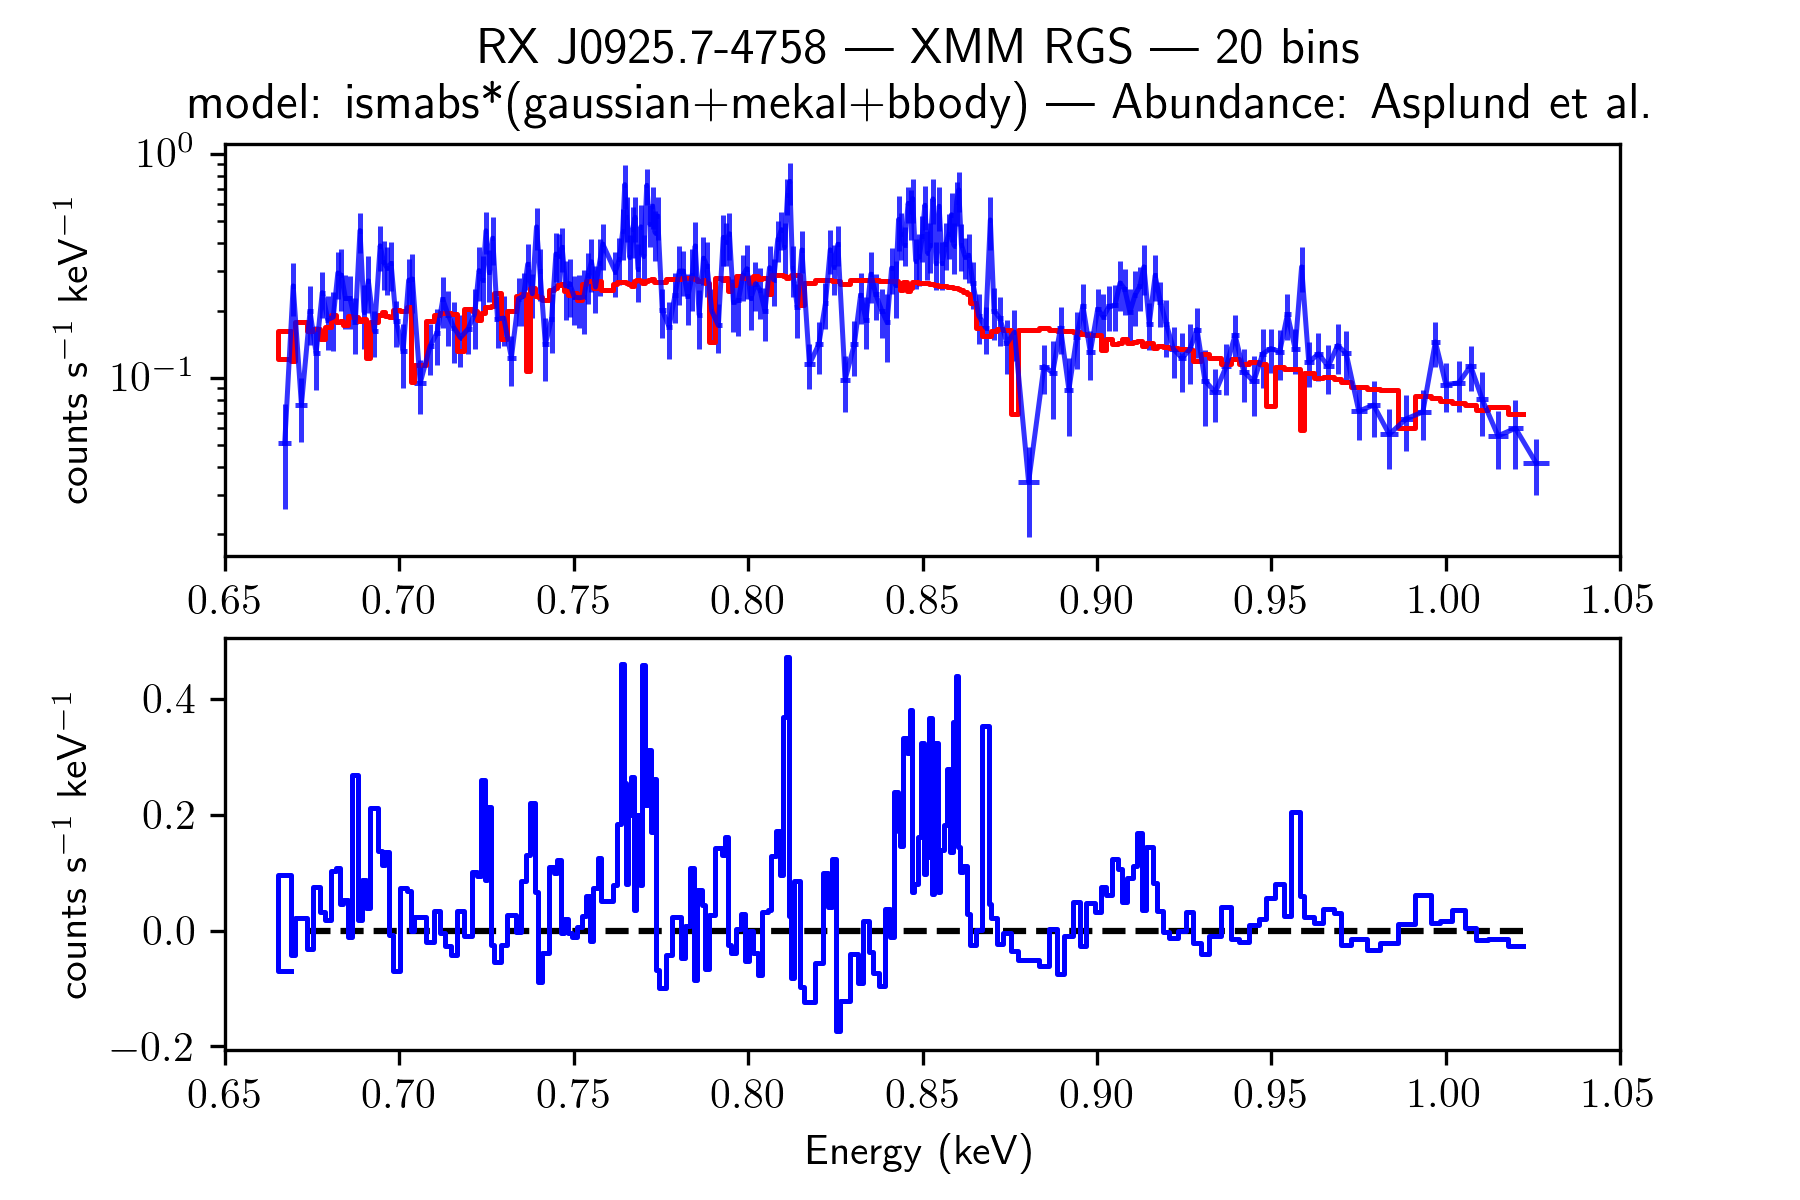
\includegraphics[width=0.9\textwidth]{mrvel-rgs2-o2-m07}} %\hfill
				\caption{Model M07 fit to RGS2 spectra}
				\label{xmm:rgs2-m07}
			\end{figure}
			
			\newpage
			\begin{figure}[h!]
				\centering
				\subfloat[Order 1 \label{xmm:rgs2-m08:o1}]{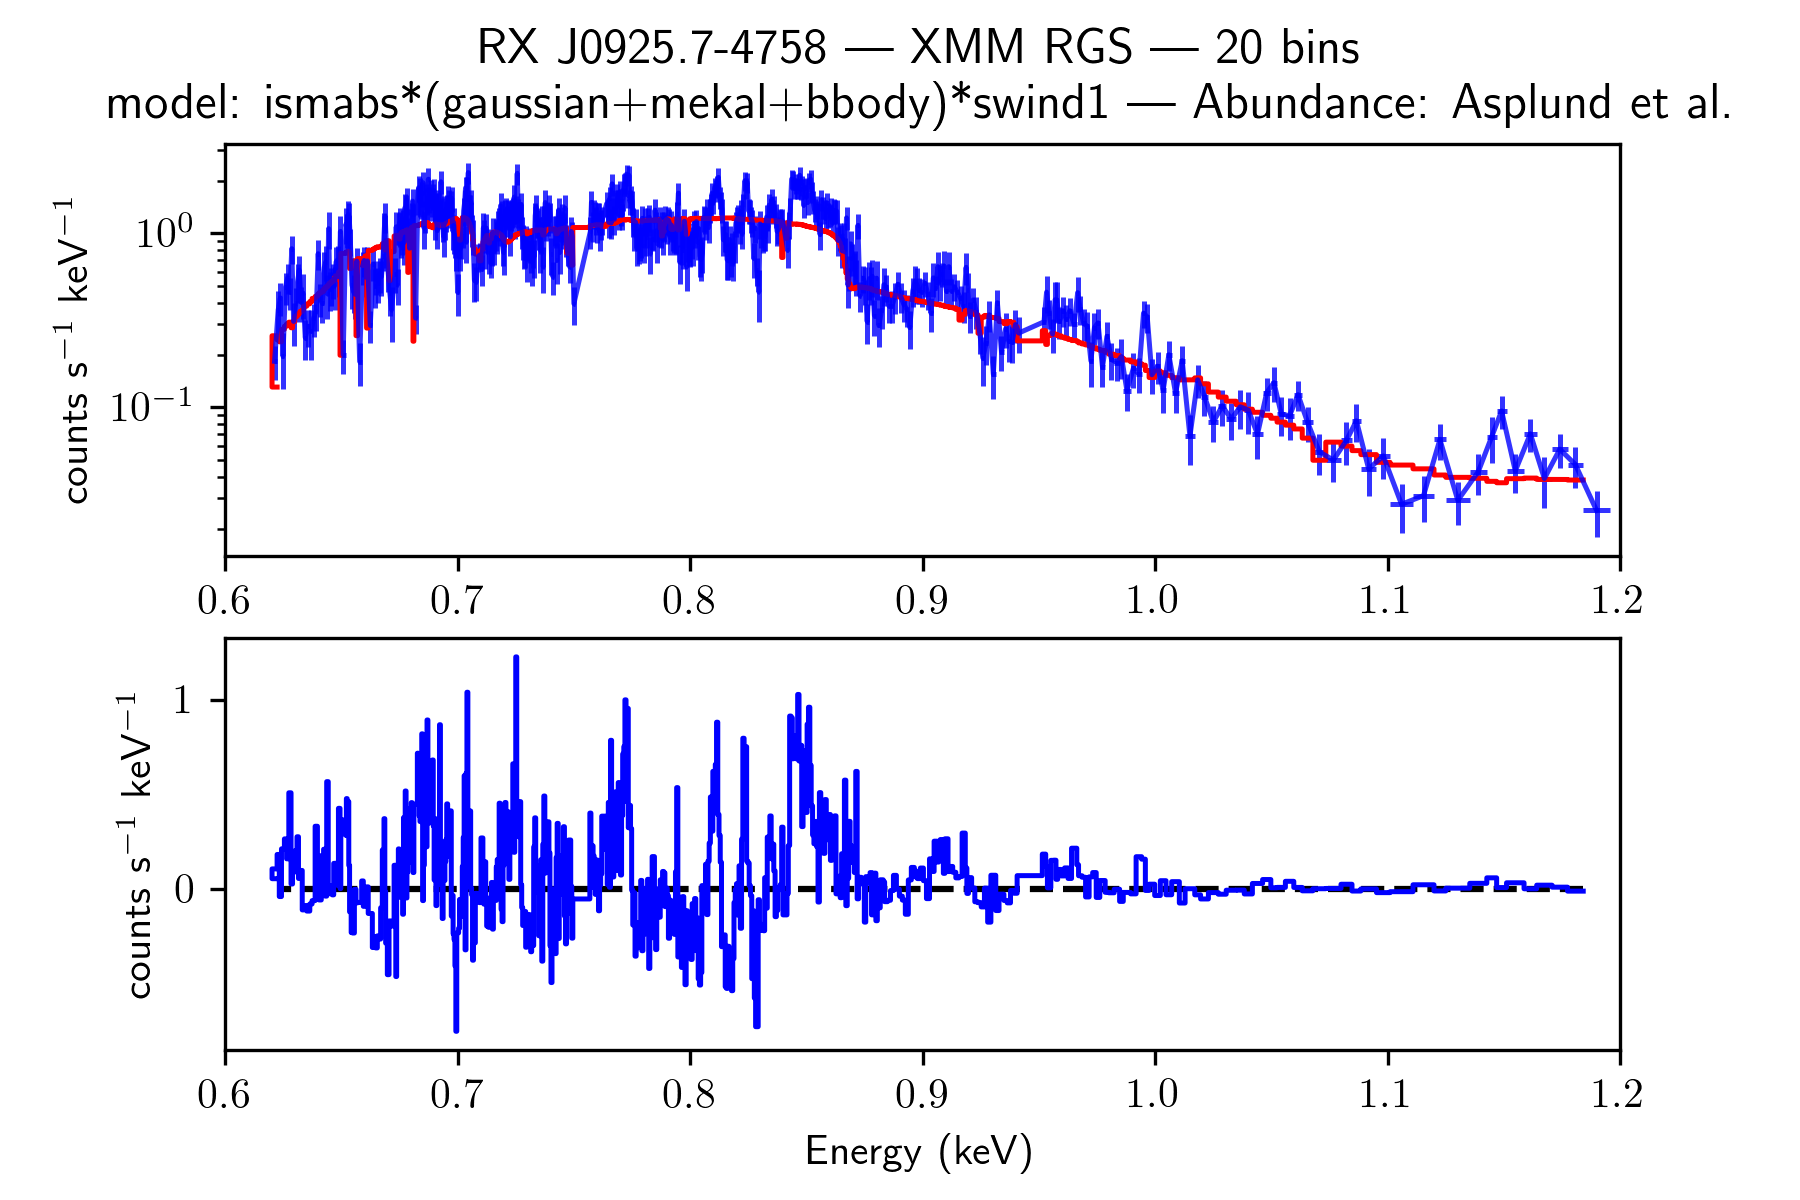
\includegraphics[width=0.9\textwidth]{mrvel-rgs2-o1-m08}} \hfill
				\subfloat[Order 2 \label{xmm:rgs2-m08:o2}]{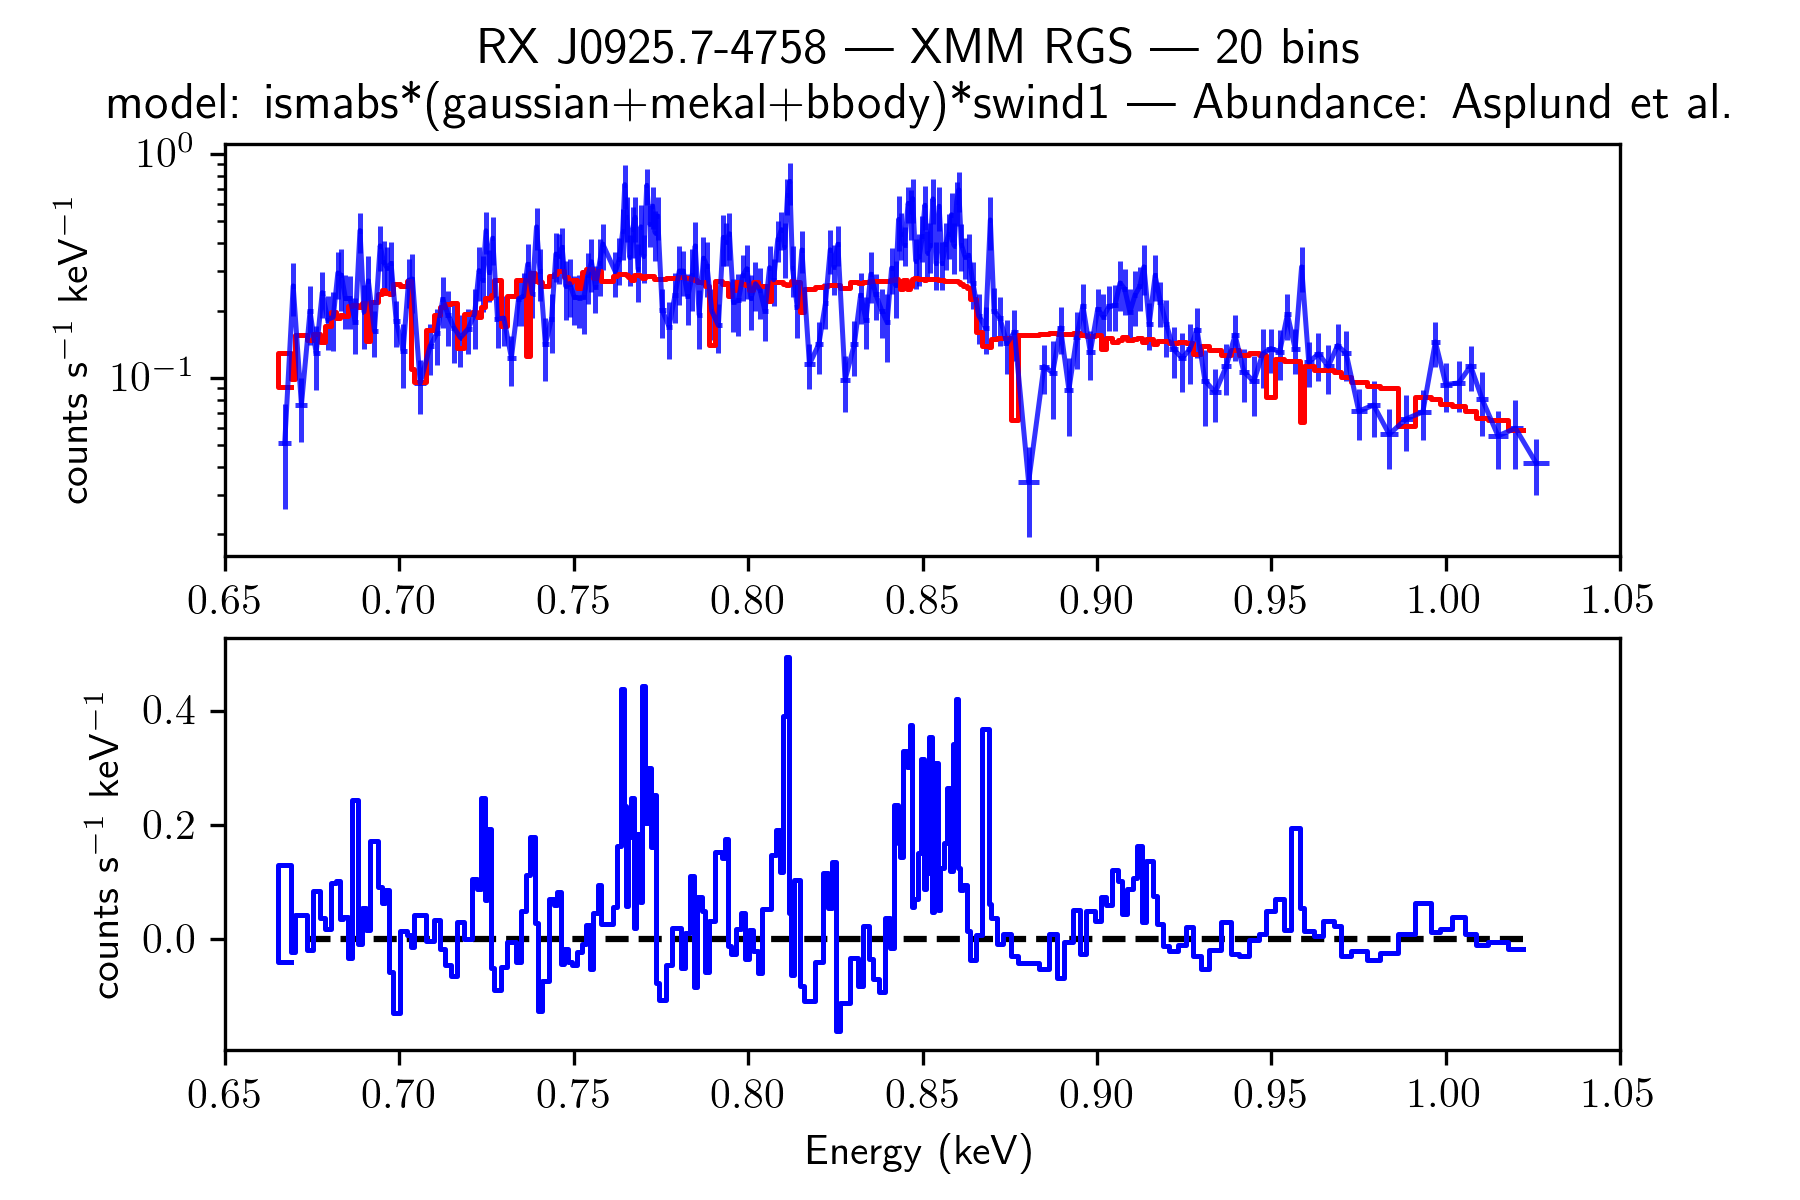
\includegraphics[width=0.9\textwidth]{mrvel-rgs2-o2-m08}} \hfill
				\caption{Model M08 fit to RGS2 spectra}
				\label{xmm:rgs2-m08}
			\end{figure}
			
			\newpage
			\begin{figure}[h!]
				\centering
				\subfloat[Order 1 \label{xmm:rgs2-m09:o1}]{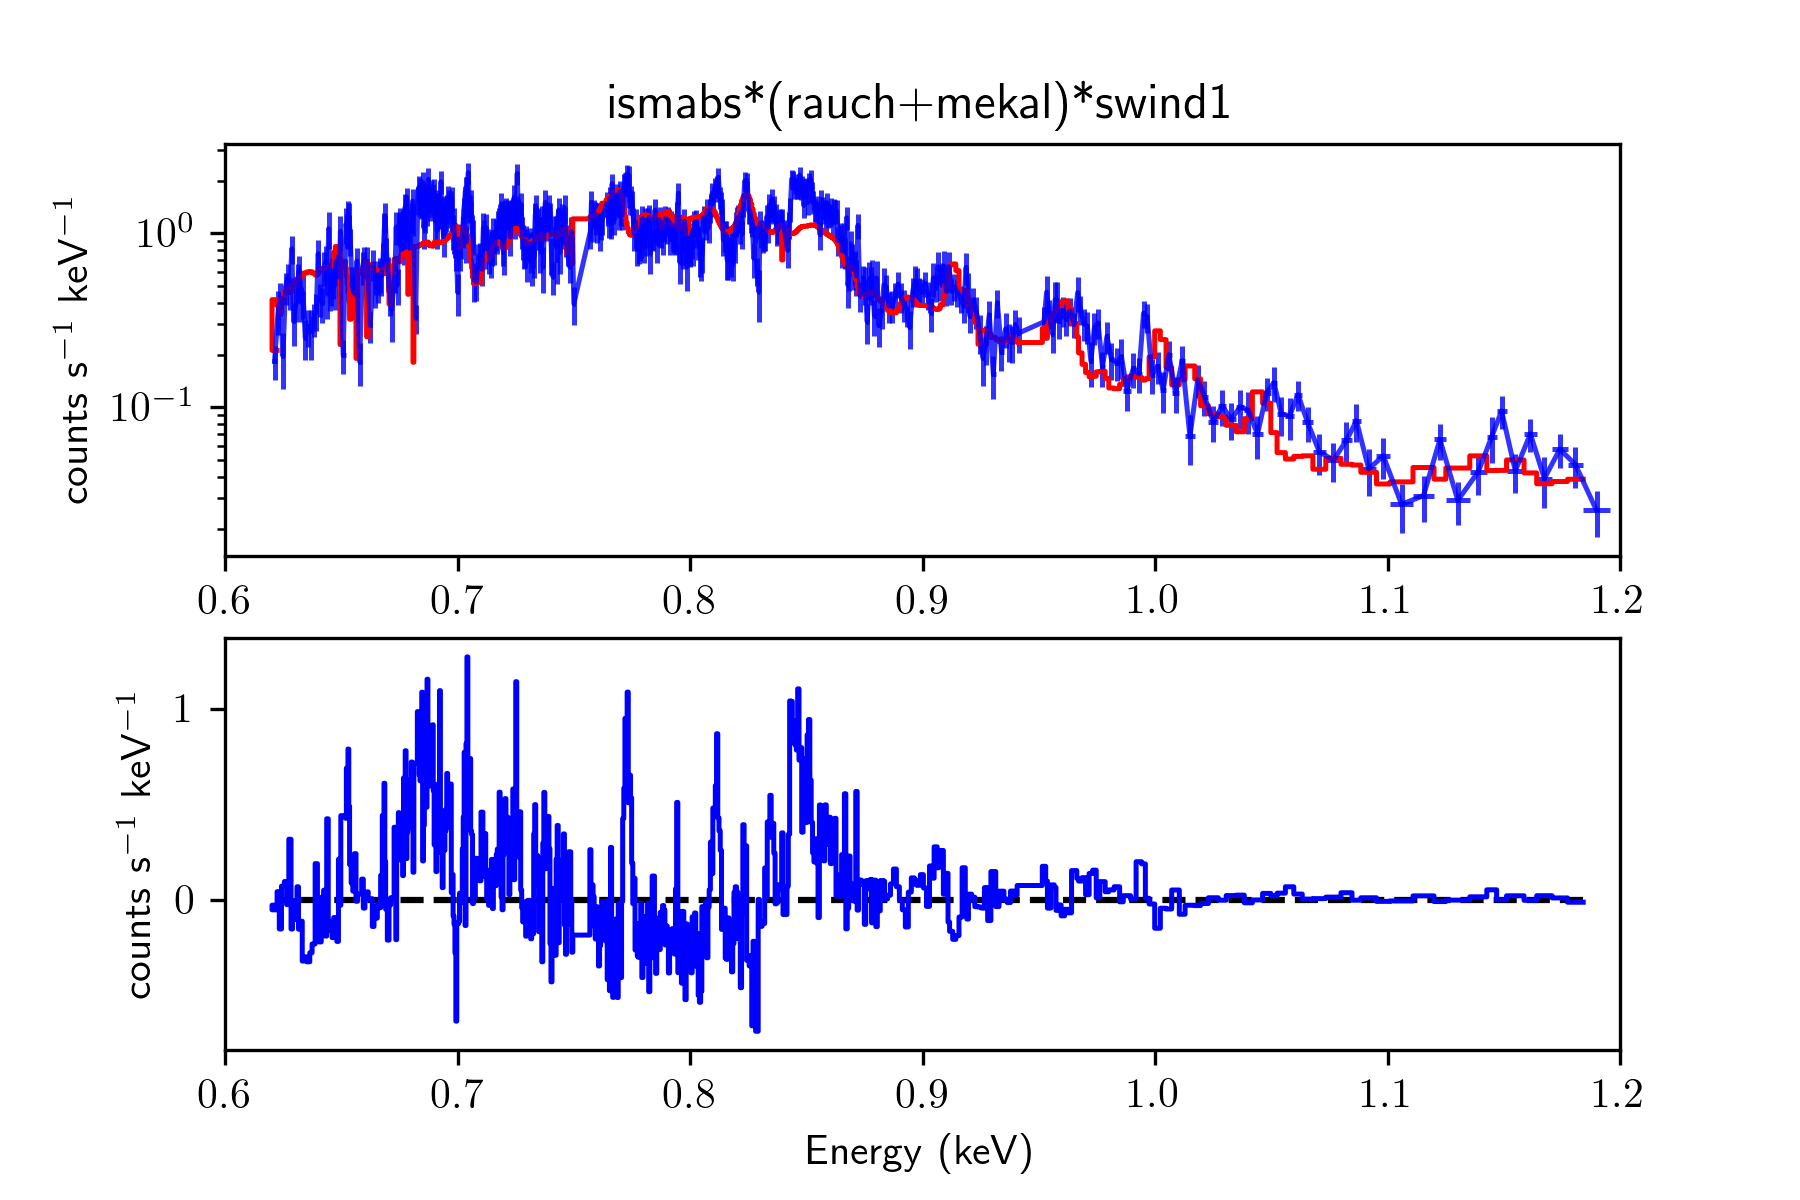
\includegraphics[width=0.9\textwidth]{mrvel-rgs2-o1-m09}} \hfill
				\subfloat[Order 2 \label{xmm:rgs2-m09:o2}]{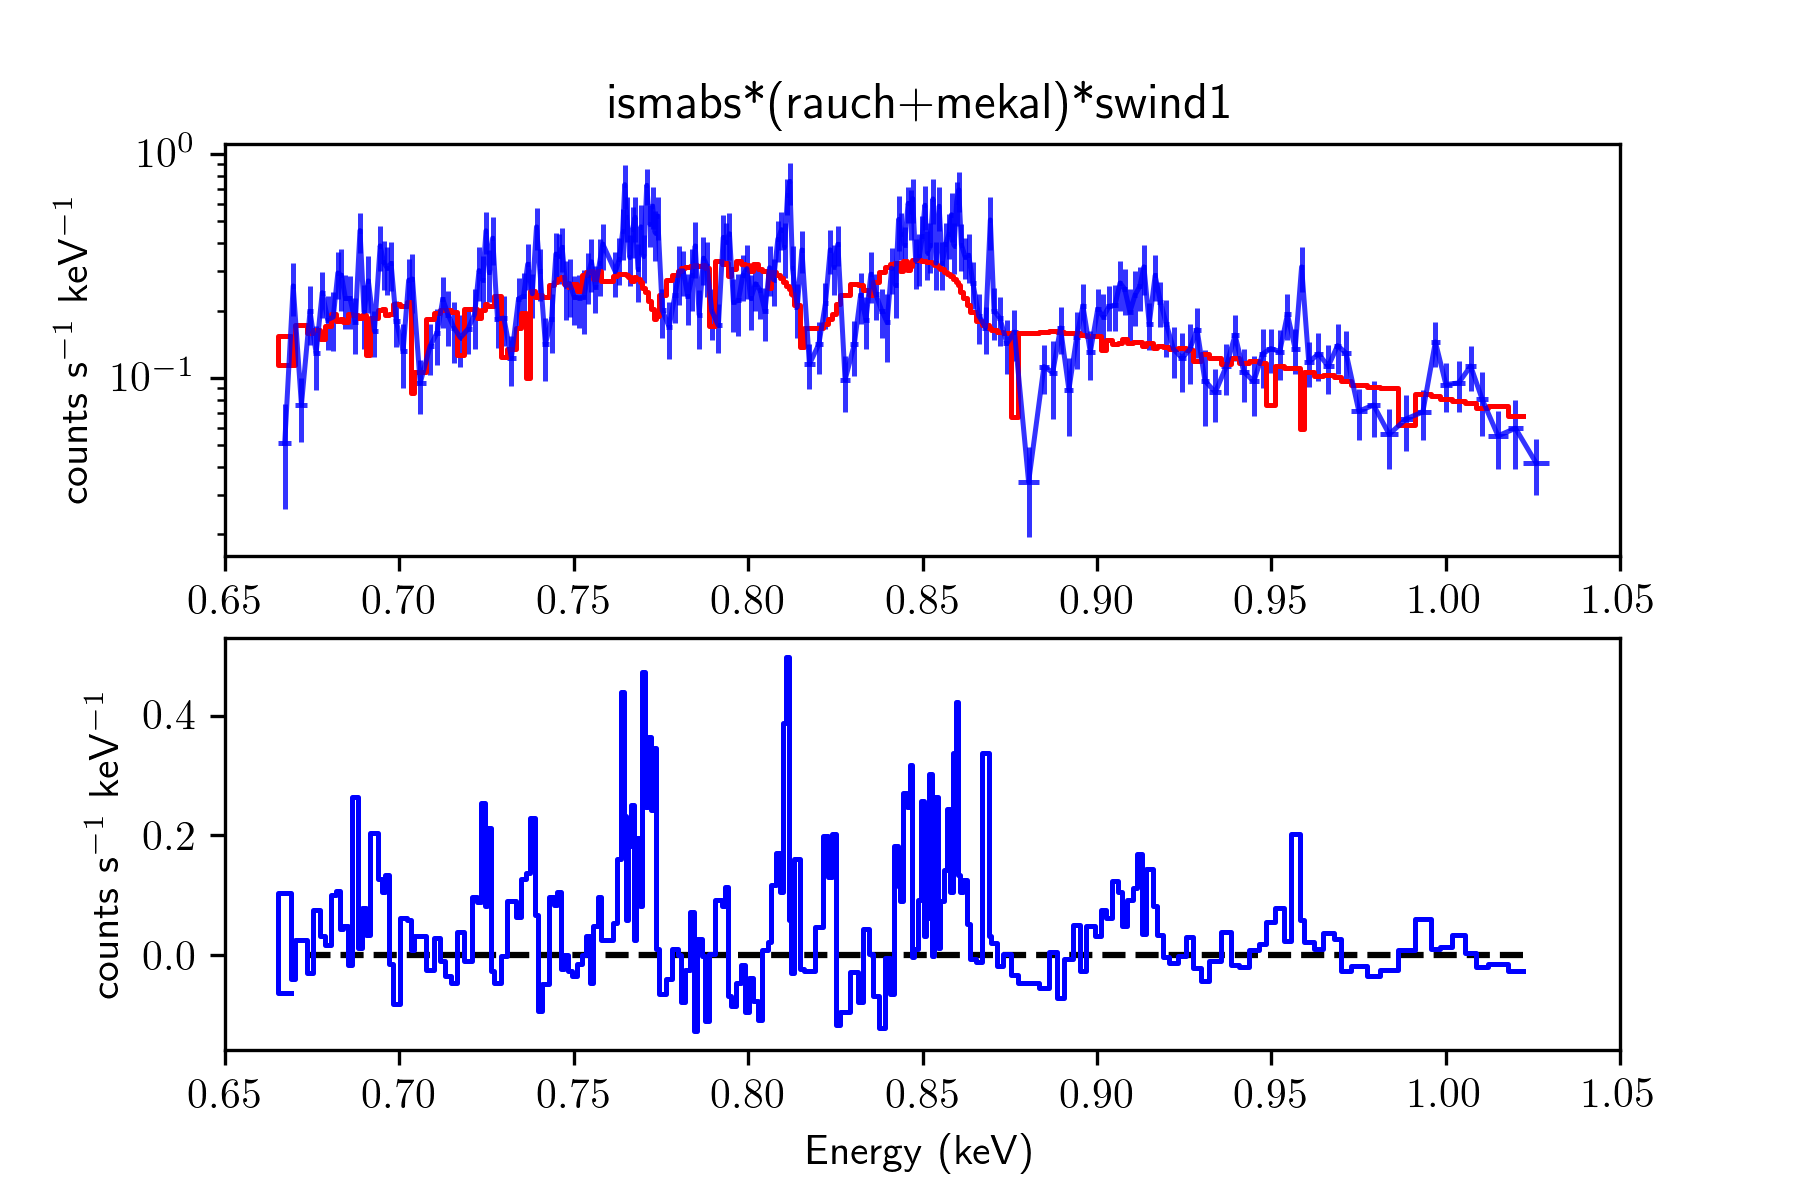
\includegraphics[width=0.9\textwidth]{mrvel-rgs2-o2-m09}} %\hfill
				\caption{Model M09 fit to RGS2 spectra}
				\label{xmm:rgs2-m09}
			\end{figure}
			
			\newpage
			\begin{figure}[h!]
				\centering
				\subfloat[Order 1 \label{xmm:rgs2-m10:o1}]{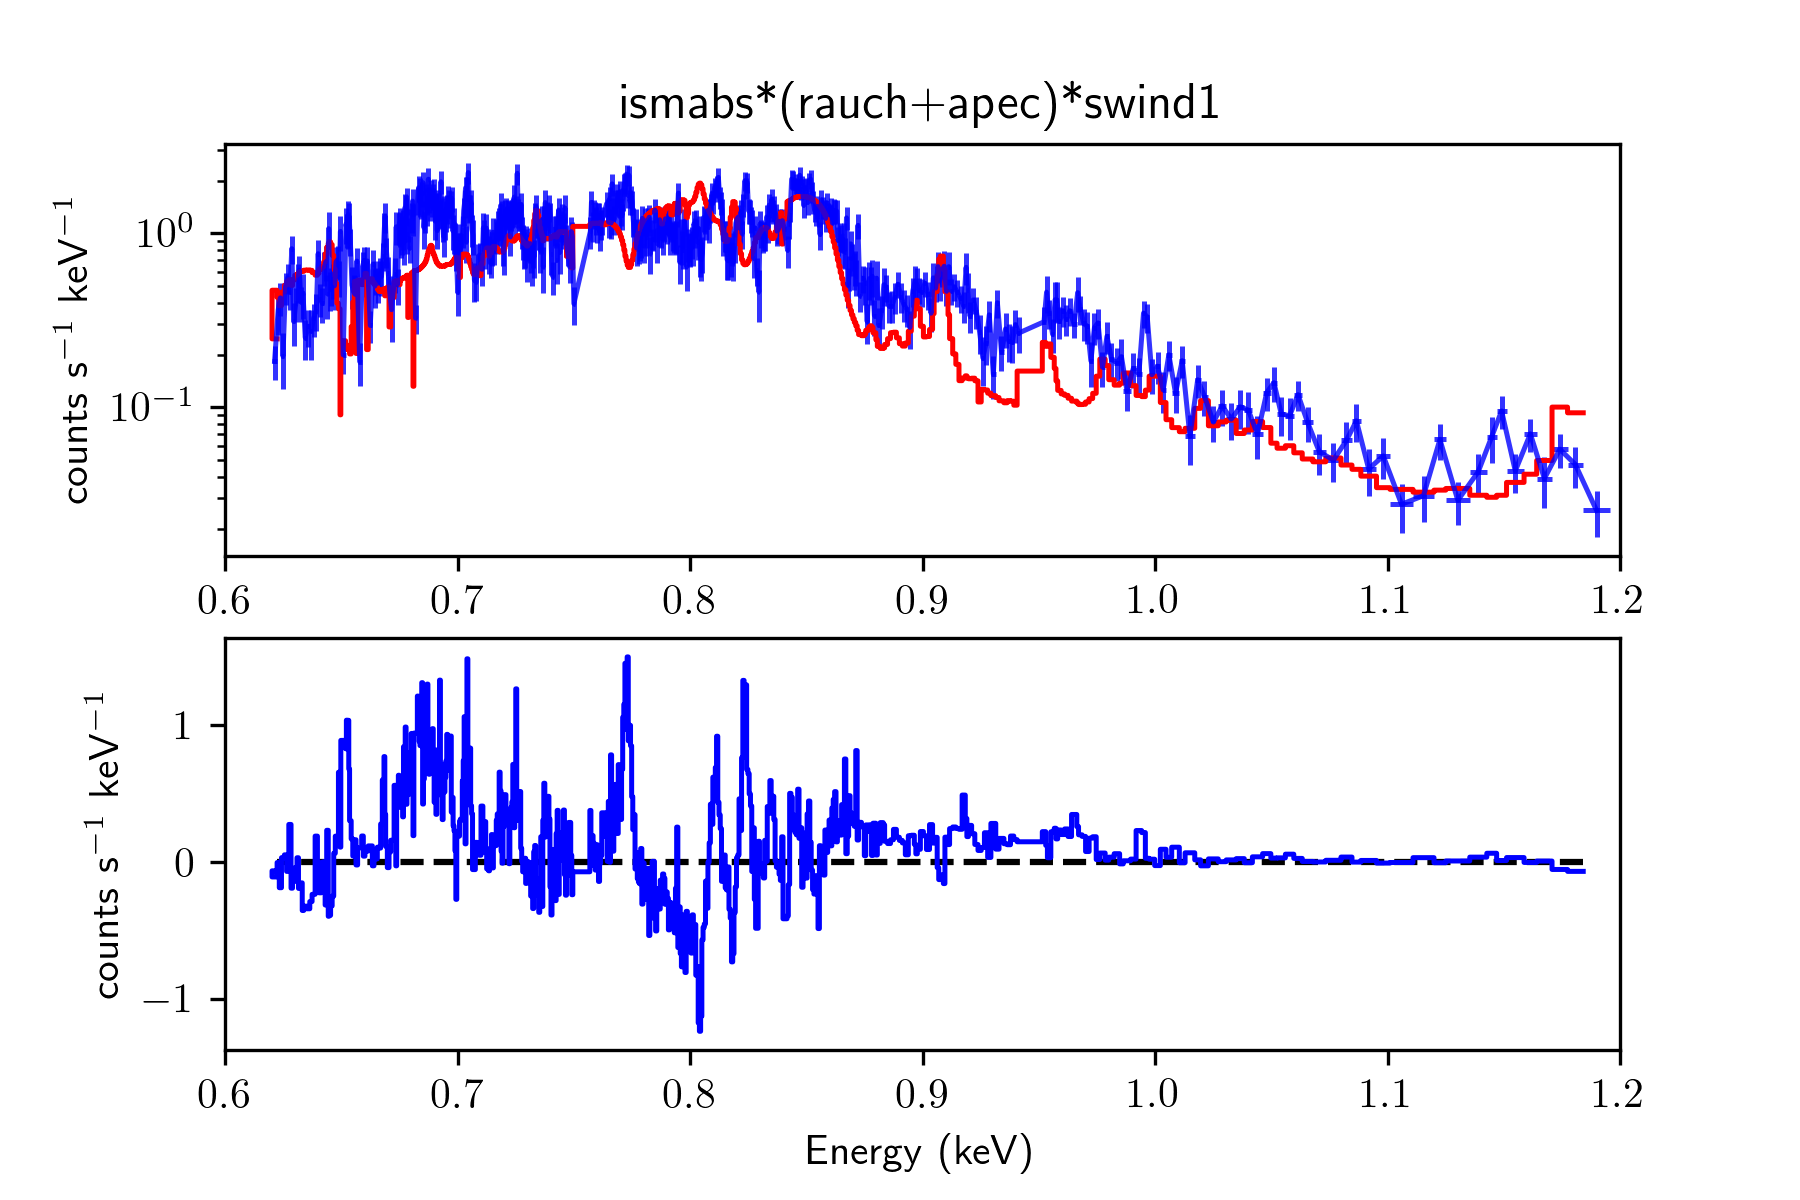
\includegraphics[width=0.9\textwidth]{mrvel-rgs2-o1-m10}} \hfill
				\subfloat[Order 2 \label{xmm:rgs2-m10:o2}]{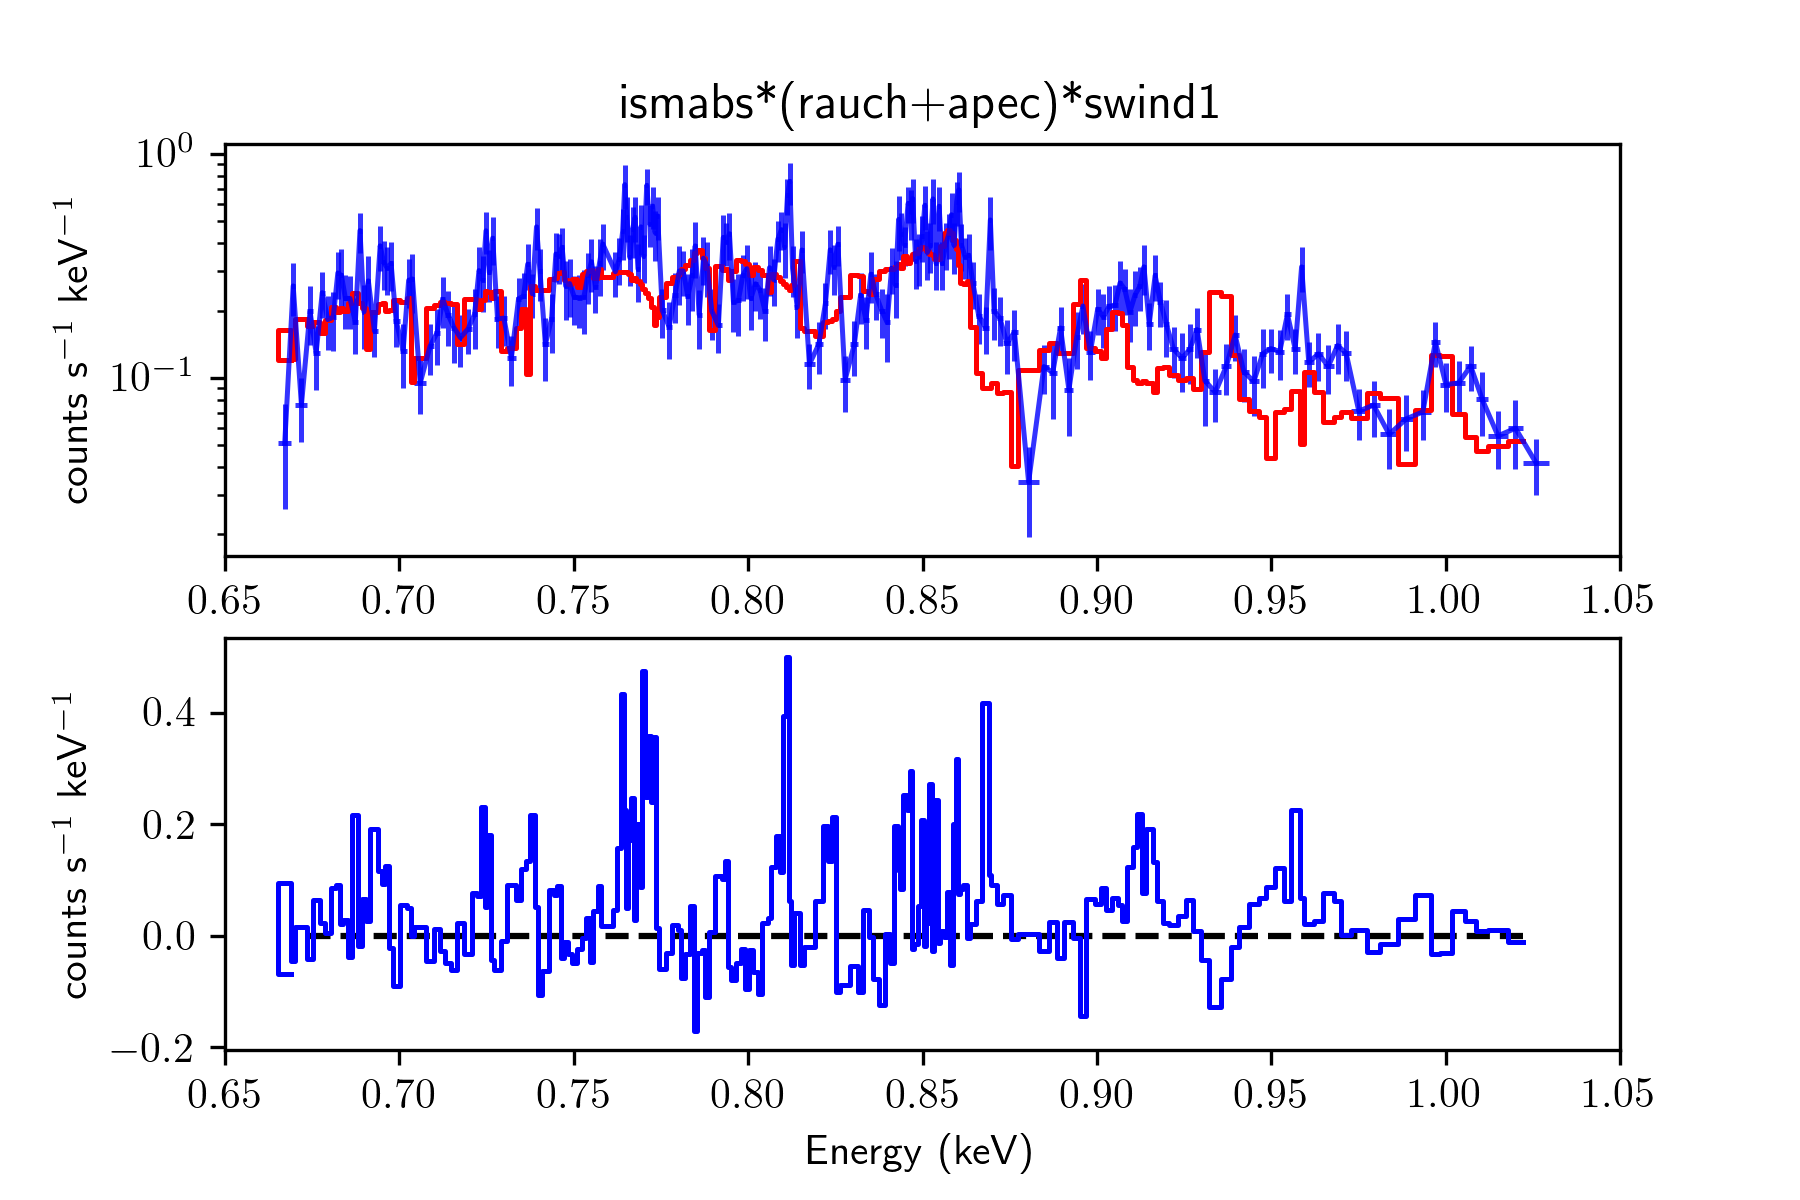
\includegraphics[width=0.9\textwidth]{mrvel-rgs2-o2-m10}} %\hfill
				\caption{Model M10 fit to RGS2 spectra}
				\label{xmm:rgs2-m10}
			\end{figure}
			
			\newpage
			\begin{figure}[h!]
				\centering
				\subfloat[Order 1 \label{xmm:rgs2-m11:o1}]{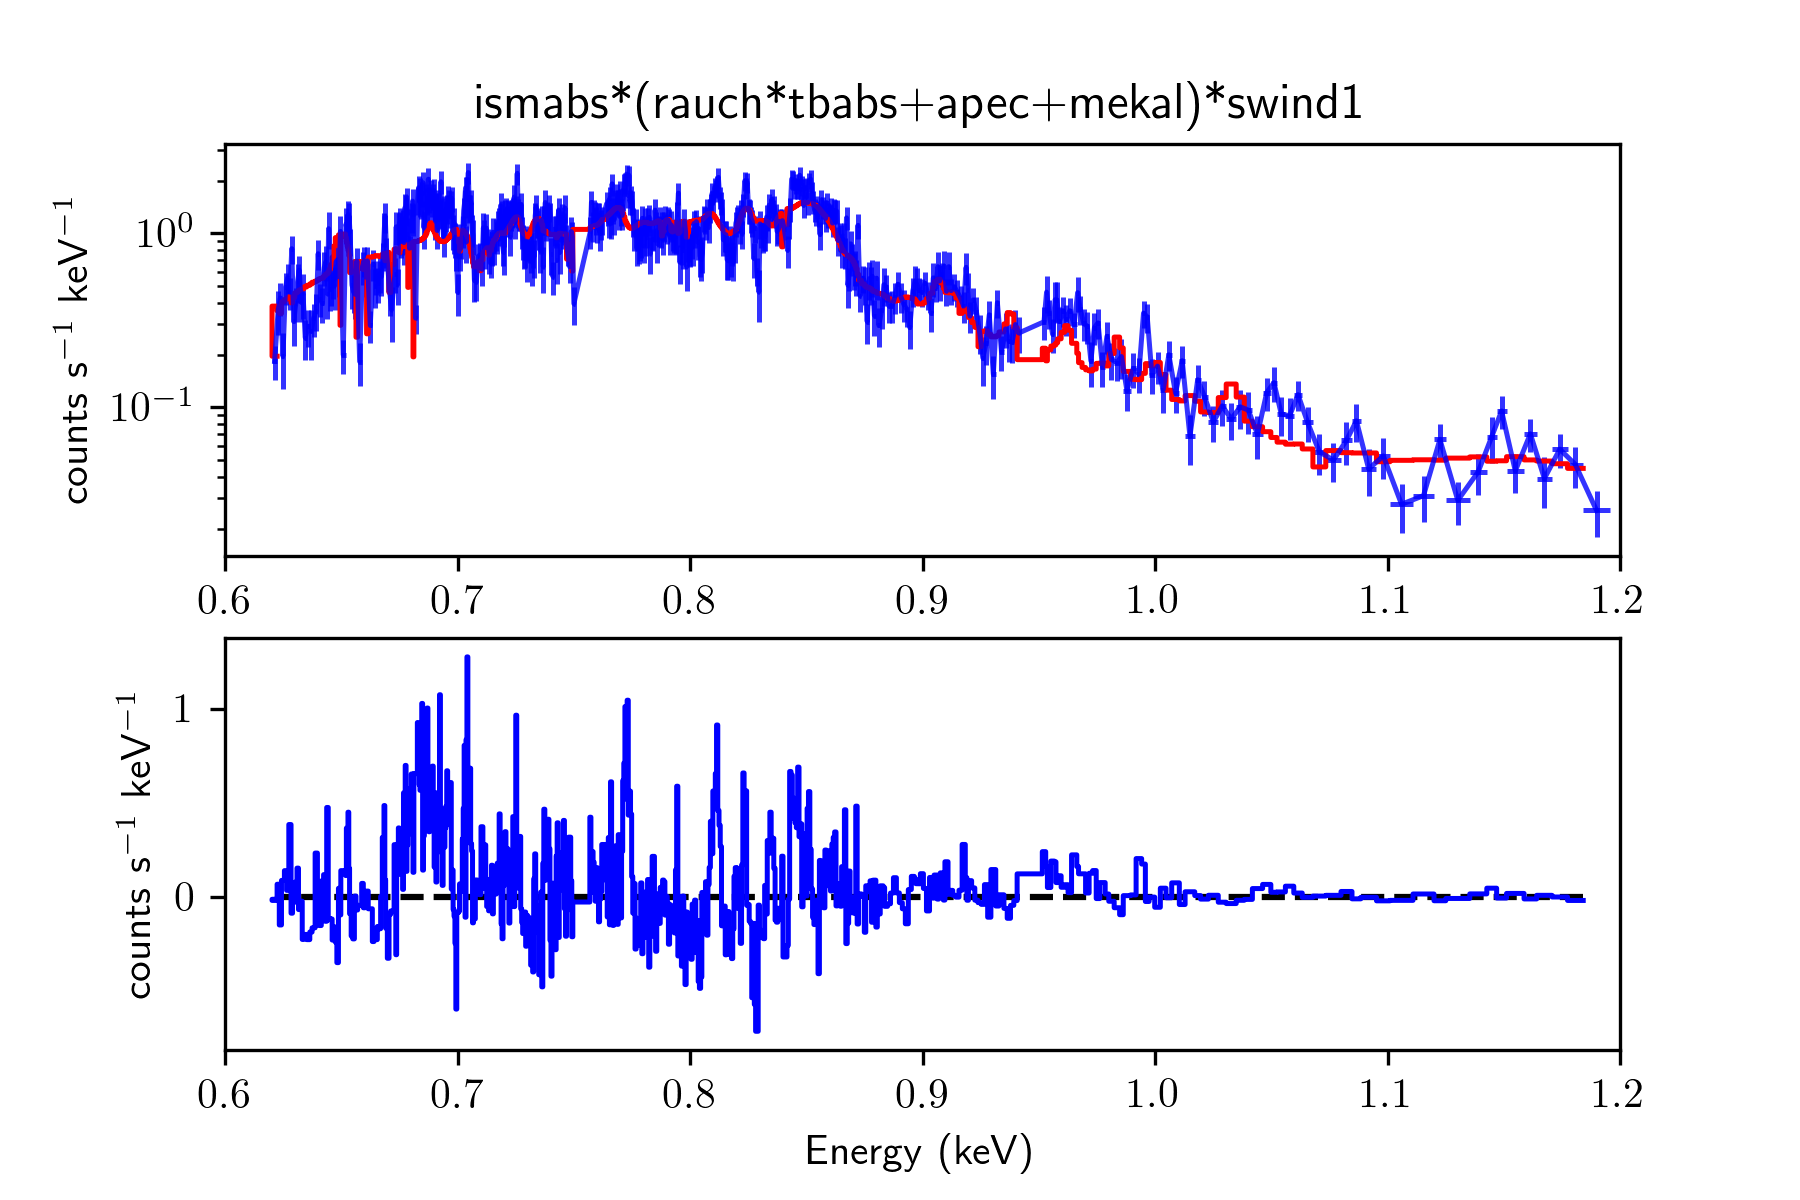
\includegraphics[width=0.9\textwidth]{mrvel-rgs2-o1-m11}} \hfill
				\subfloat[Order 2 \label{xmm:rgs2-m11:o2}]{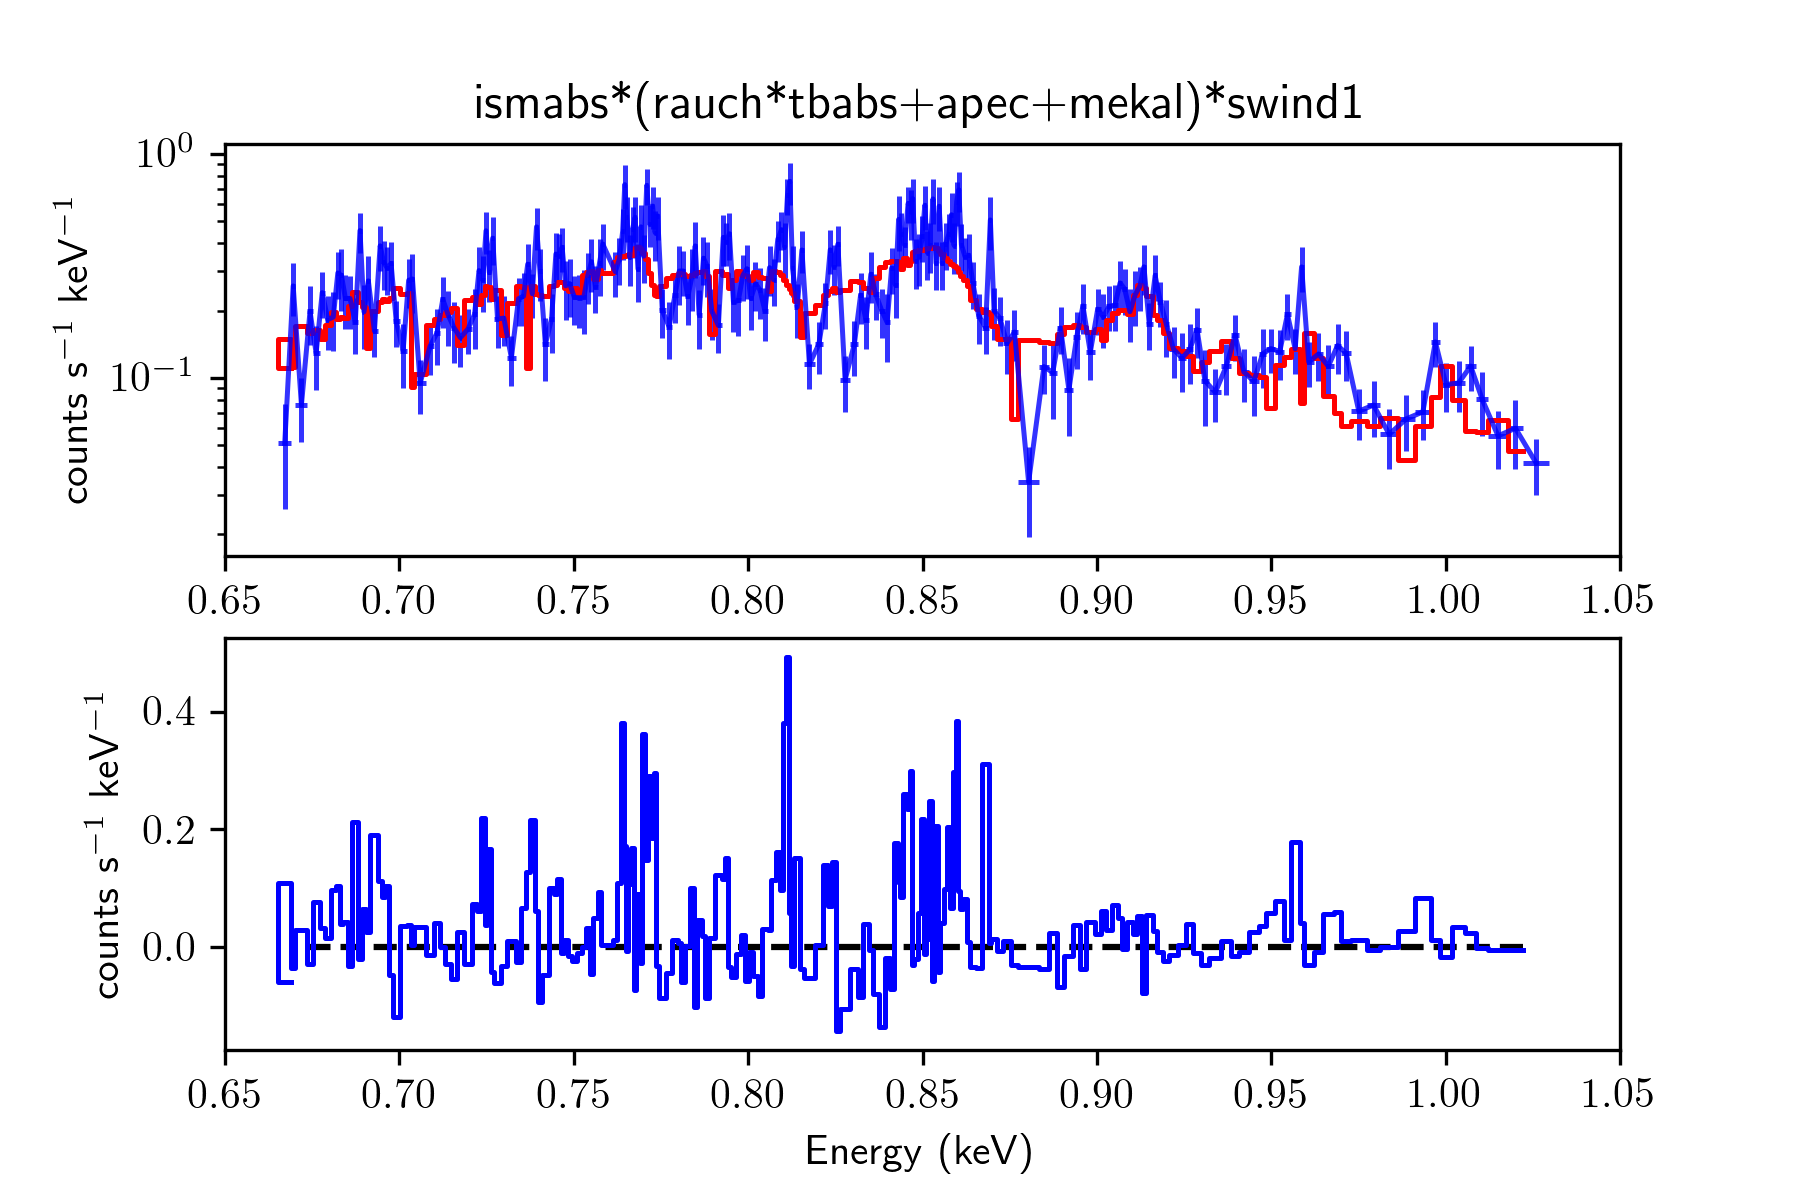
\includegraphics[width=0.9\textwidth]{mrvel-rgs2-o2-m11}} %\hfill
				\caption{Model M11 fit to RGS2 spectra}
				\label{xmm:rgs2-m11}
			\end{figure}
			
			\newpage
			\begin{figure}[h!]
				\centering
				\subfloat[Order 1 \label{xmm:rgs2-m12:o1}]{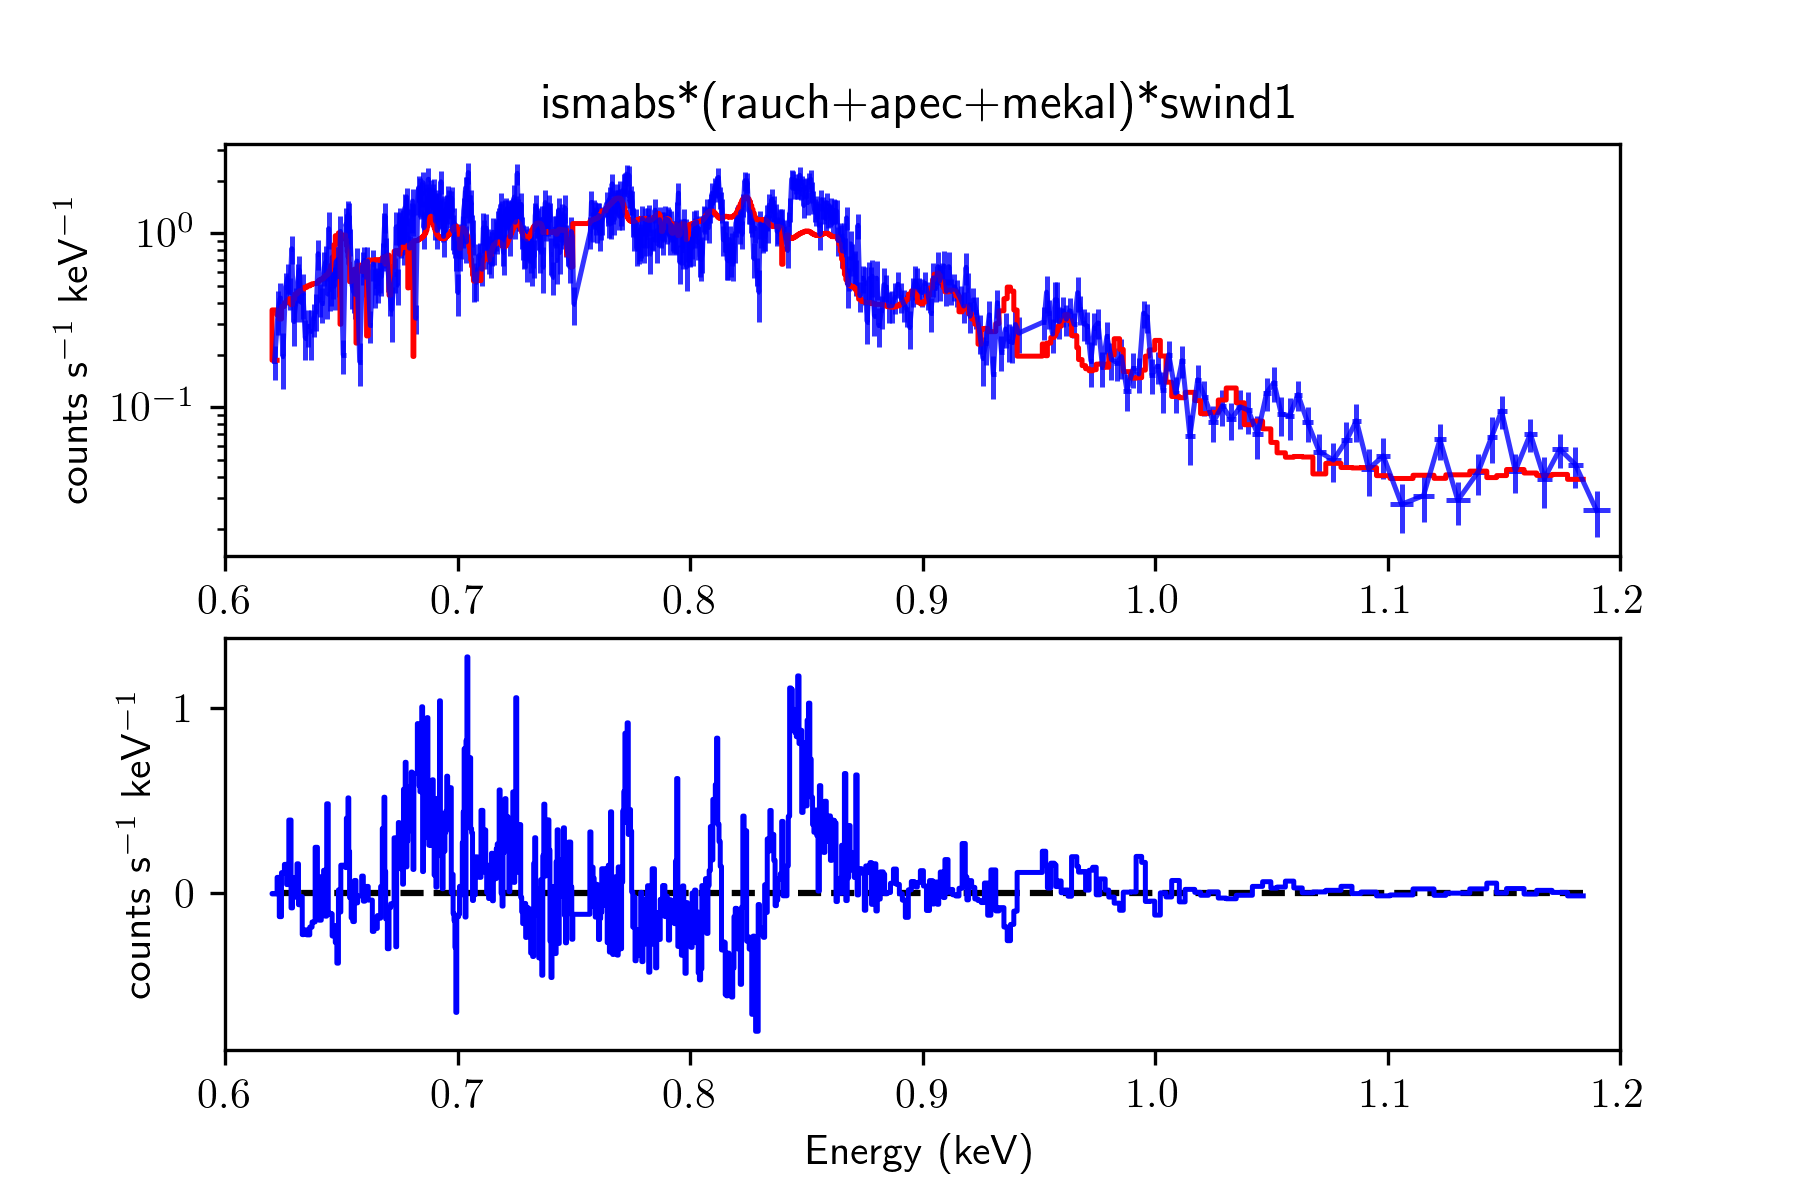
\includegraphics[width=0.9\textwidth]{mrvel-rgs2-o1-m12}} \hfill
				\subfloat[Order 2 \label{xmm:rgs2-m12:o2}]{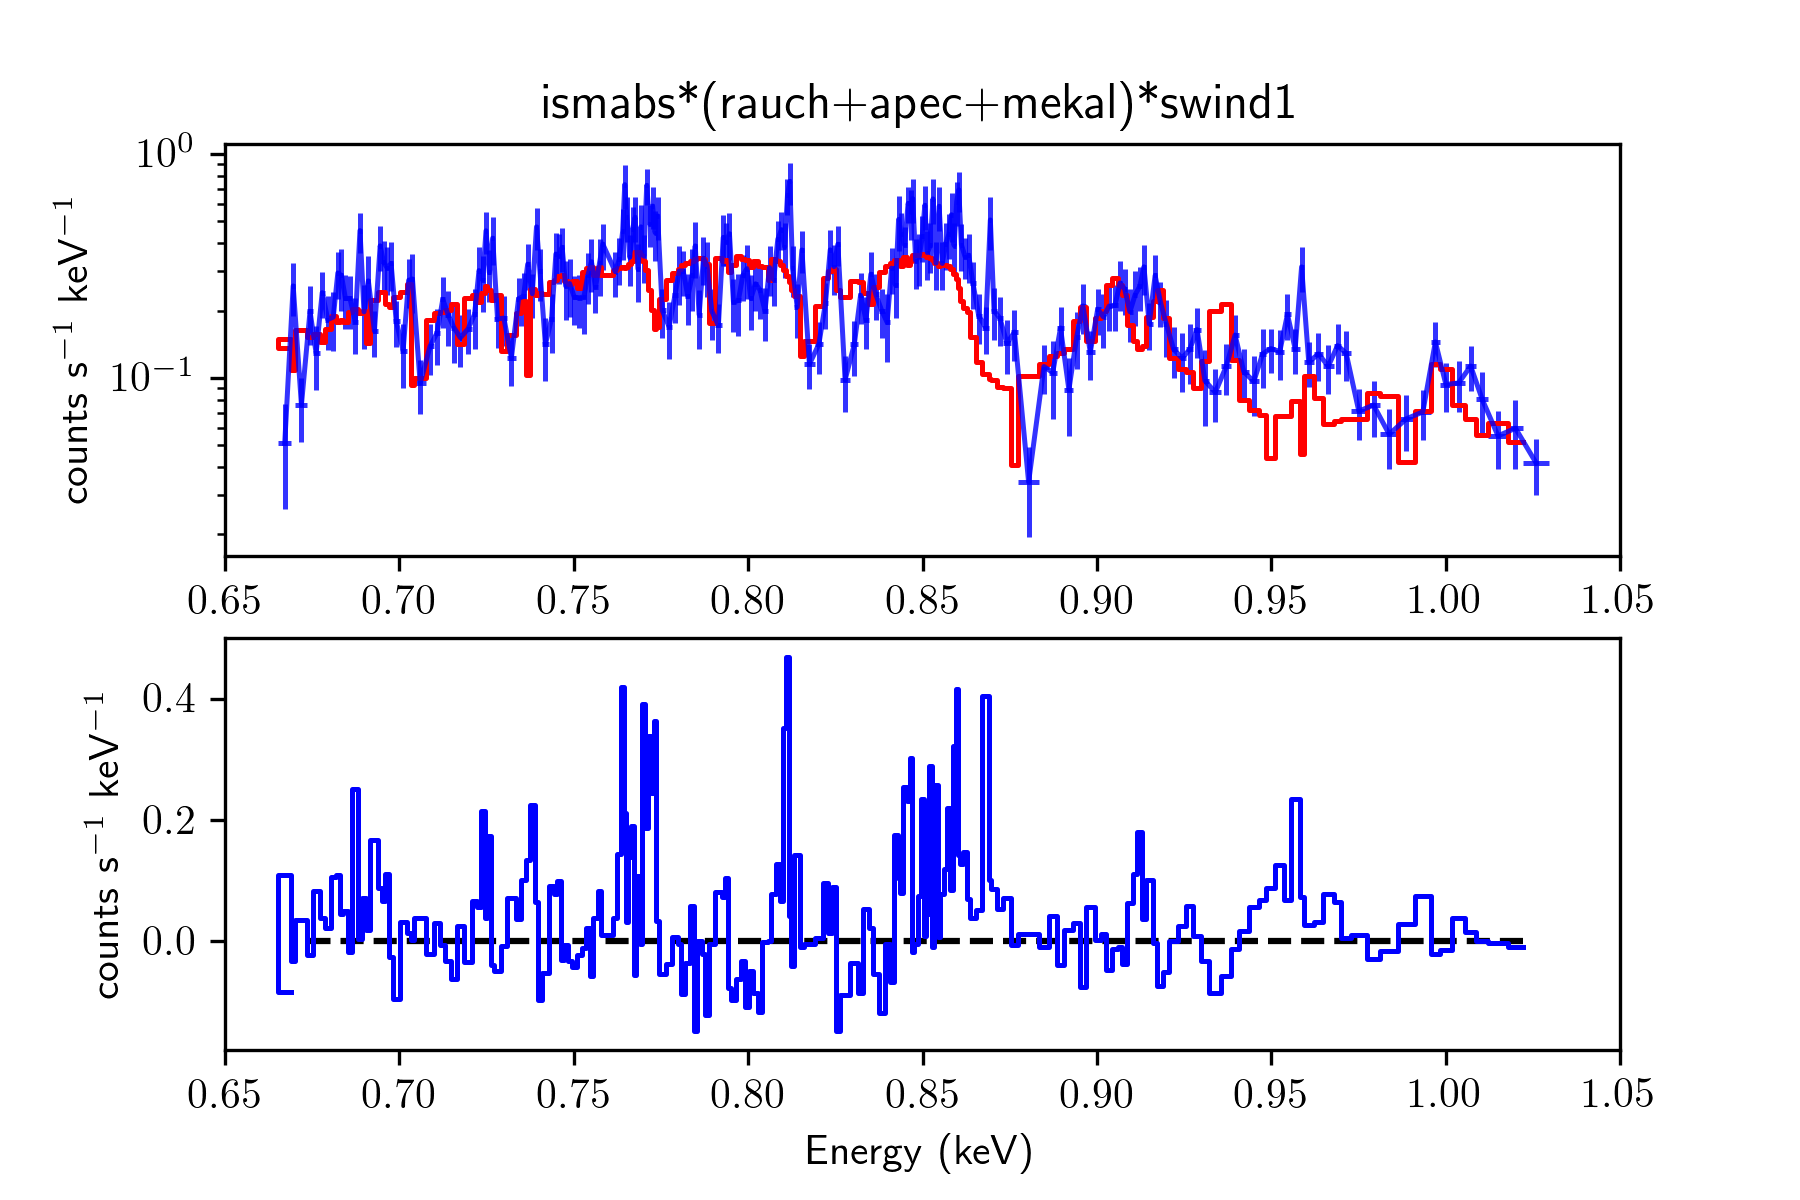
\includegraphics[width=0.9\textwidth]{mrvel-rgs2-o2-m12}} %\hfill
				\caption{Model M12 fit to RGS2 spectra}
				\label{xmm:rgs2-m12}
			\end{figure}
			
		\subsection{Comparison with Current Literature}
			Here we present a comparison of the quality of the spectral fit achieved in this work with those reported in previous studies. Table \ref{tab:mrvel-fit:comparison} summarizes the reduced chi-squared ($\chi^2_\text{reduced}$) values for the best-fitting model (M11) from our analysis, alongside results from existing literature.
			%In table \ref{tab:mrvel-fit:comparison}, we present a comparison of the best-fit statistics of the best performing model from our grid with results given in existing literature.
			\begin{table}[!htb]
				\centering
				\caption{Comparison of best-fit statistics of RGS spectra from RX J0925.7-4758}
				\label{tab:mrvel-fit:comparison}
				\begin{tabular}{llc}
					\hline
					\multicolumn{2}{l}{\textbf{Title of work}} & $\boldsymbol{\chi^2_\text{reduced}}$ \\ \hline
					\multicolumn{2}{l}{Ebisawa \etal\ (1996)} & 10.0 \\ %\hline
					\multicolumn{2}{l}{Bearda \etal\ (2002)} & Not quoted \\ %\hline
					\multicolumn{2}{l}{Motch \etal\ (2002)} & Not quoted \\ \hline
					\multicolumn{1}{l|}{\multirow{4}{*}{\begin{tabular}[c]{@{}l@{}}M11\\
						(current work)\end{tabular}}} & RGS1 (order 1) & {2.36} \\ %\cline{2-3}
						\multicolumn{1}{l|}{} & RGS1 (order 2) & {1.66} \\ %\cline{2-3}
						\multicolumn{1}{l|}{} & RGS2 (order 1) & {2.14} \\ %\cline{2-3}
						\multicolumn{1}{l|}{} & RGS2 (order 2) & {1.80} \\ \hline
				\end{tabular}
			\end{table}			
					
			As table \ref{tab:mrvel-fit:comparison} illustrates, the $\chi^2_\text{reduced}$ values obtained for model M11 in this work (ranging from 1.66 to 2.36) are significantly lower than the value reported by Ebisawa \etal\ (1996) \cite{ebisawa1996}.  Bearda \etal\ (2002) and Motch \etal\ (2002) do not provide $\chi^2_\text{reduced}$ values in their studies, merely reporting the near impossibility of modelling the RGS spectrum of RX J0925.7-4758 using an NLTE model atmosphere \cite{beardaChandra2002AA,motchXmmNewton2002AA}.  The substantial improvement in fit quality achieved here suggests that model M11 seems to offer a more accurate representation of the physical processes governing the X-ray emission from RX J0925.7-4758.
			%As it is evident, the model M11 seems to provide a far better fit to the RGS spectra, as compared to existing literature. This model can be written mathematically as:
			
			Mathematically, the expression for model M11 can be written as,
			\begin{center}
				\texttt{ismabs*(rauch*tbabs+apec+mekal)*swind1}
			\end{center}
			
		\subsection{Supersoft X-ray Physics Using Best-fit RGS Model}
			The model M11, by virtue of its individual components, sheds light on the physical mechanisms responsible for the X-ray emission observed from RX J0925.7-4758. The \texttt{ismabs} term specifically accounts for the partial absorption of X-rays along the line of sight due to the interstellar medium (ISM). The ISM, comprising primarily gas and dust, attenuates the incoming X-ray photons before they reach the object, effectively weakening the observed X-ray flux.
			
			Delving deeper into RX J0925.7-4758, the \texttt{rauch*tbabs} component sheds light on the intrinsic X-ray emission. The \texttt{tbabs} element maintains its role as a standard model for photoelectric absorption by cold, denser gas within the object. However, the \texttt{rauch} term introduces a new layer of complexity. It represents an emission component arising from a non-local thermodynamic equilibrium (NLTE) atmosphere, which captures the effects of this specific atmospheric model on the X-ray emission. This suggests that the intrinsic X-ray emission from RX J0925.7-4758 might not be uniform but influenced by the properties of this NLTE atmosphere, potentially caused by deviations from thermal equilibrium within the emitting gas.
			
			The narrative of X-ray emission from RX J0925.7-4758 takes a significant turn with the inclusion of both \texttt{apec} and \texttt{mekal} terms. These terms represent distinct thermal plasma emission models. \texttt{Apec} is indicative of optically thin plasma, where the surrounding gas is relatively sparse. In such an environment, X-rays have a higher probability of traveling freely with minimal interactions before inducing radiative emission. \texttt{Mekal}, on the other hand, is suited for modeling thicker plasma regions. Here, X-rays are more likely to collide with particles within the gas, leading to a different emission mechanism. The presence of both models in the model M11 suggests that the hot gas surrounding RX J0925.7-4758 might exhibit variations in density. Consequently, the X-ray emission from this hot gas could potentially originate from two distinct processes depending on the local plasma conditions.
			
			The final component, i.e. \texttt{swind1}, adds a layer of complexity by incorporating the possibility of deviations from a uniform velocity field within the emitting gas. This term suggests the presence of internal motions within the hot gas surrounding RX J0925.7-4758. These motions could be due to various factors, such as turbulence, bulk flows, or outflows. Including \texttt{swind1} recognizes the dynamic nature of the emitting region and suggests the need for more complex models. %The inclusion of \texttt{swind1} acknowledges the dynamic nature of the emitting region and highlights the potential need for more sophisticated modeling approaches to fully characterize the physical processes at play.
			
%		\subsection{With Order 1 Spectrum} \label{hi-resolution:analysis:order-1}
%			The 1$^{\mathrm{st}}$ order diffraction spectrum was fitted using the six models mentioned in \S\ref{hi-resolution:analysis} in the same order. The progression of the models increased the number of parameters, in spite of which there seems to be an improvement in the fit, as compared to those in available in literature. The best fit also seems to show significant abundances for NeI, MgI and ArI, at $2.87\times 10^{18}$, $1.10\times 10^{18}$ and $5.35\times 10^{18}$ respectively, as compared to the other metals included in the model.
%			
%			\begin{figure}[h!]
%				\centering
%				\caption{Fitted spectrum using composite model}
%				\subfloat[\texttt{ismabs*edge*edge*edge*(gaussian+bbody)} \label{xmm-rgs:01}]{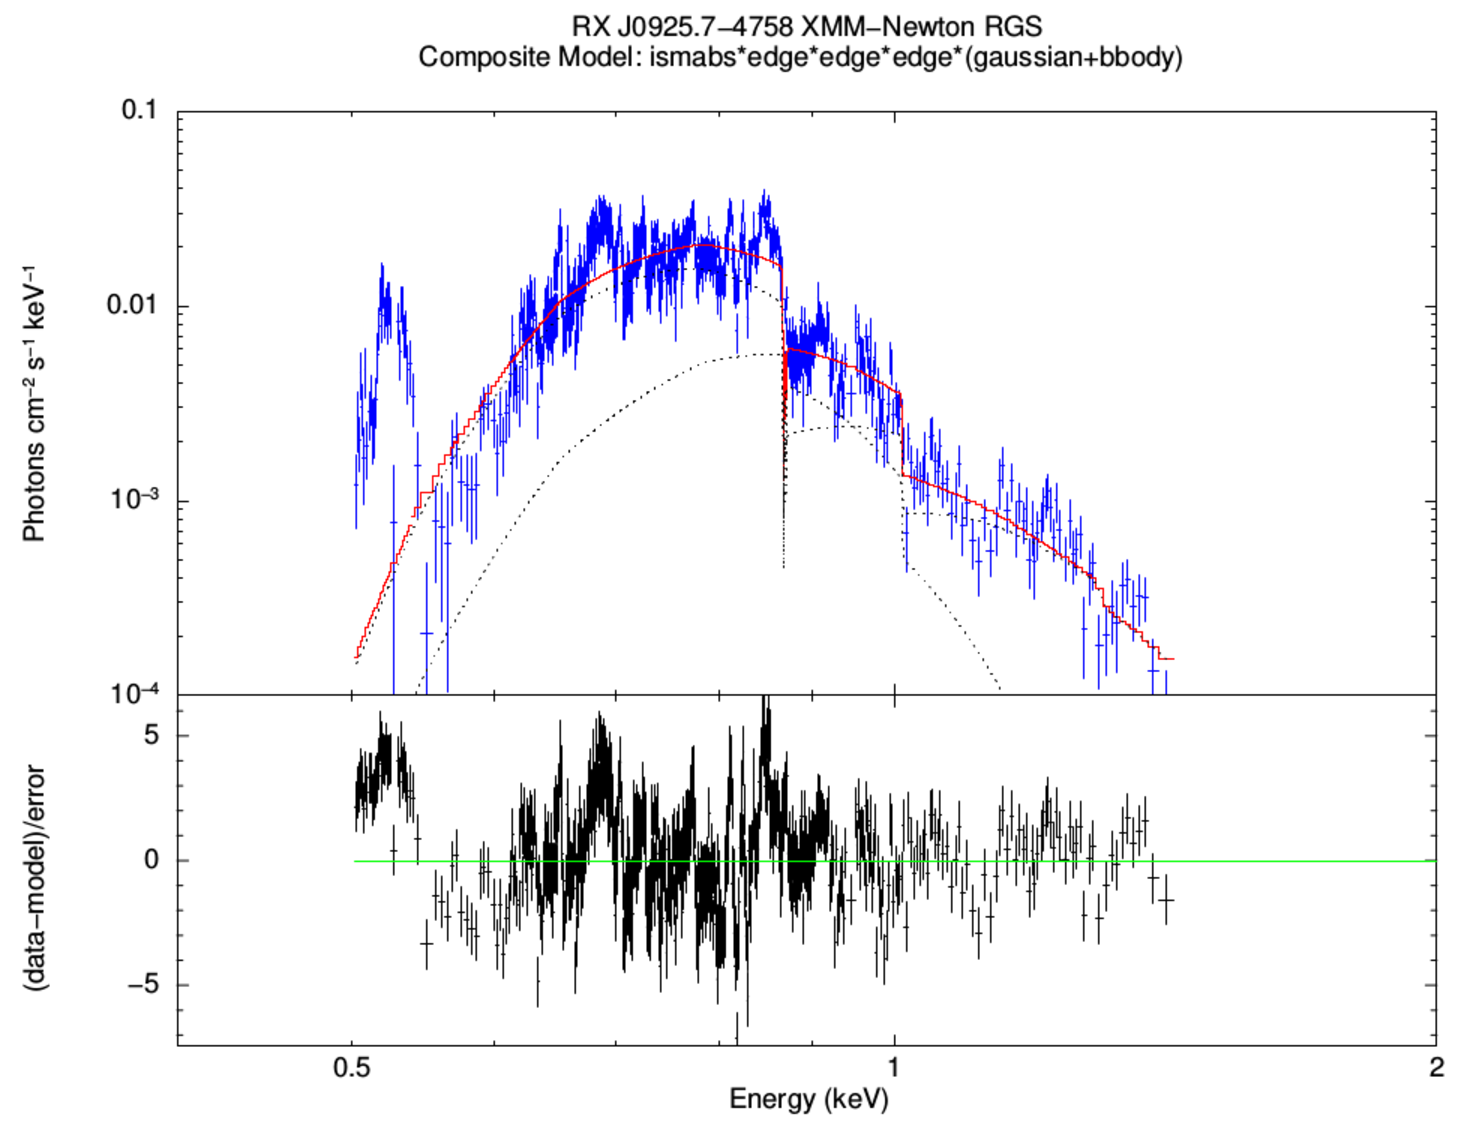
\includegraphics[scale=0.45]{mr-vel-xmm-rgs-01.pdf}}
%			\end{figure}
%			
%			But there are large deviations, especially for the softer X-ray photons. This is mainly because of the fact that the current model only incorporates continuum components. To fit the large number of observed lines in the spectrum, one needs to also include model components that account for emission lines. The additive model \texttt{mekal} computes an emission spectrum from hot diffuse optical plasma (perhaps a hot corona) based on the model calculations of Mewe, Kaastra and Liedahl. The \texttt{gaussian} component is replaced with \texttt{mekal} and an attempt was made to fit the same spectrum again.
%			\begin{figure}[h!]
%				\centering
%				\caption{Fitted spectrum using composite model}
%				\subfloat[\texttt{ismabs*edge*edge*edge*(mekal+bbody)} \label{xmm-rgs:02}]{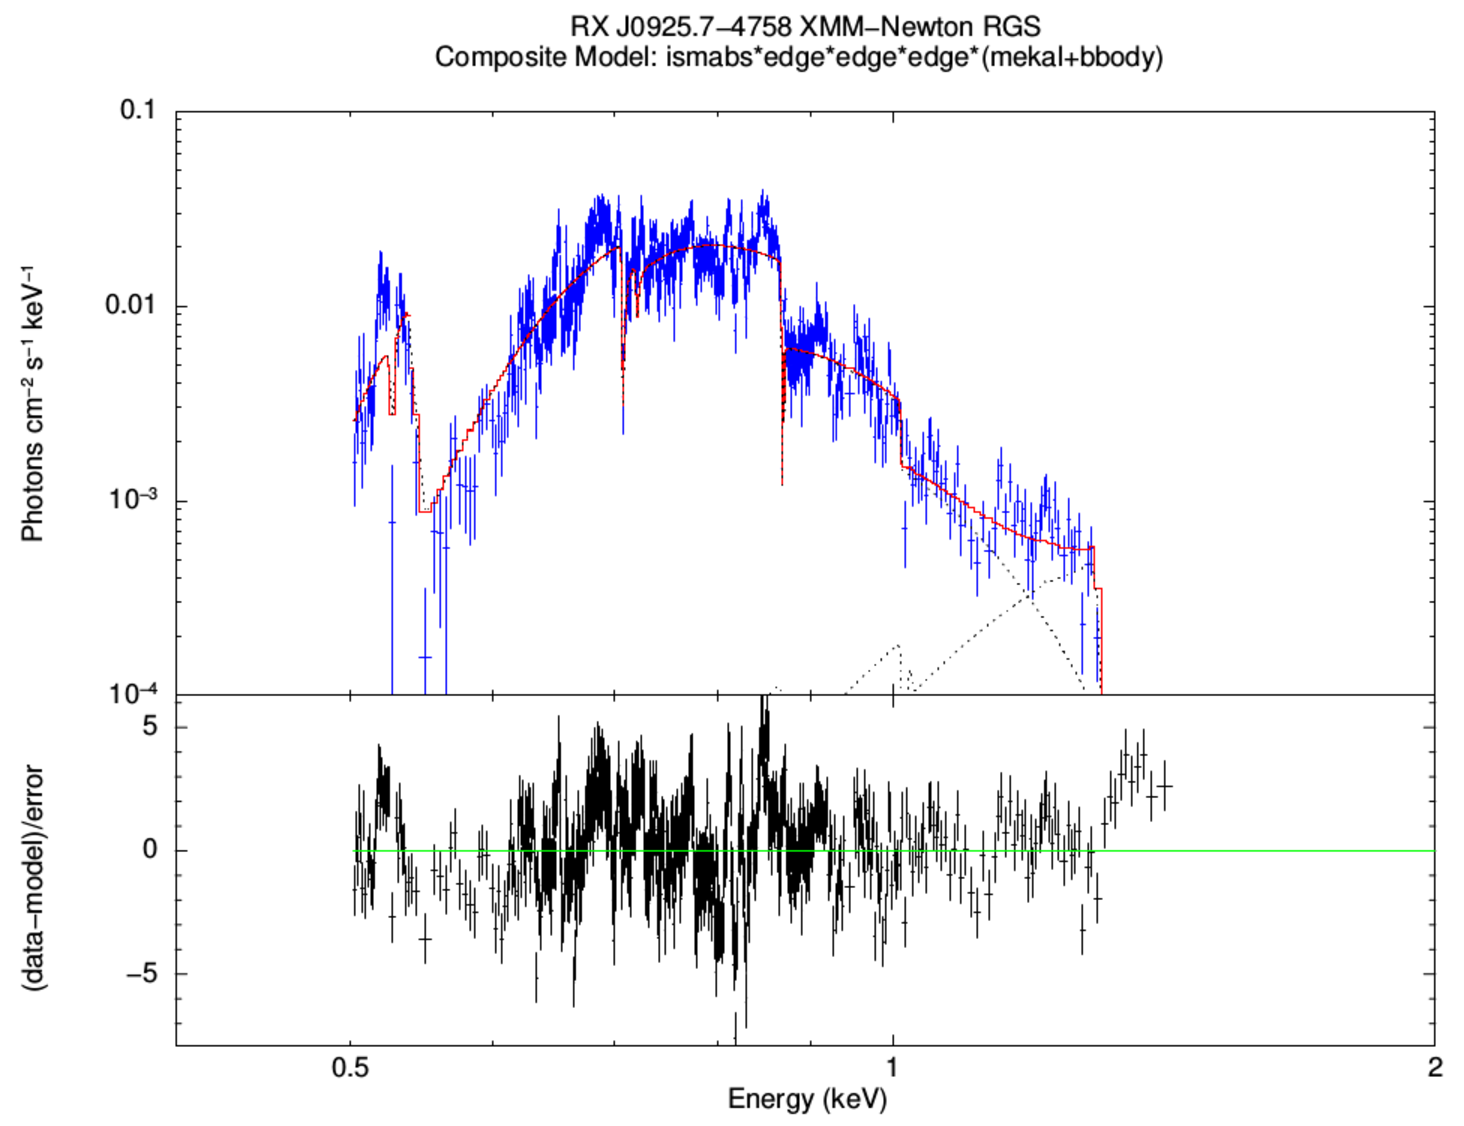
\includegraphics[scale=0.45]{mr-vel-xmm-rgs-02.pdf}}
%			\end{figure}
%			
%			An improvement in the fit was observed, with a reduced $\chi^2$ value of 3.81. A visual inspection of the fitted spectrum shows that the softer photons have been accounted for with this model. This model also seems to show significant abundances for OI, NeI, MgI and SiI at $5.57\times 10^{18}$, $3.06\times 10^{18}$, $3.84\times 10^{19}$ and $7.02\times 10^{18}$ respectively.
%
%		\subsection{With Order 2 Spectrum} \label{hi-resolution:analysis:order-2}
%			The previous composite model was used to fit the 2$^{\mathrm{nd}}$ order diffraction spectrum, with a maximum grouping of 20 bins.
%			
%			\begin{figure}[h!]
%				\centering
%				\caption{Fitted spectrum using composite model}
%				\subfloat[\texttt{ismabs*edge*edge*edge*(mekal+bbody)} \label{xmm-rgs:03}]{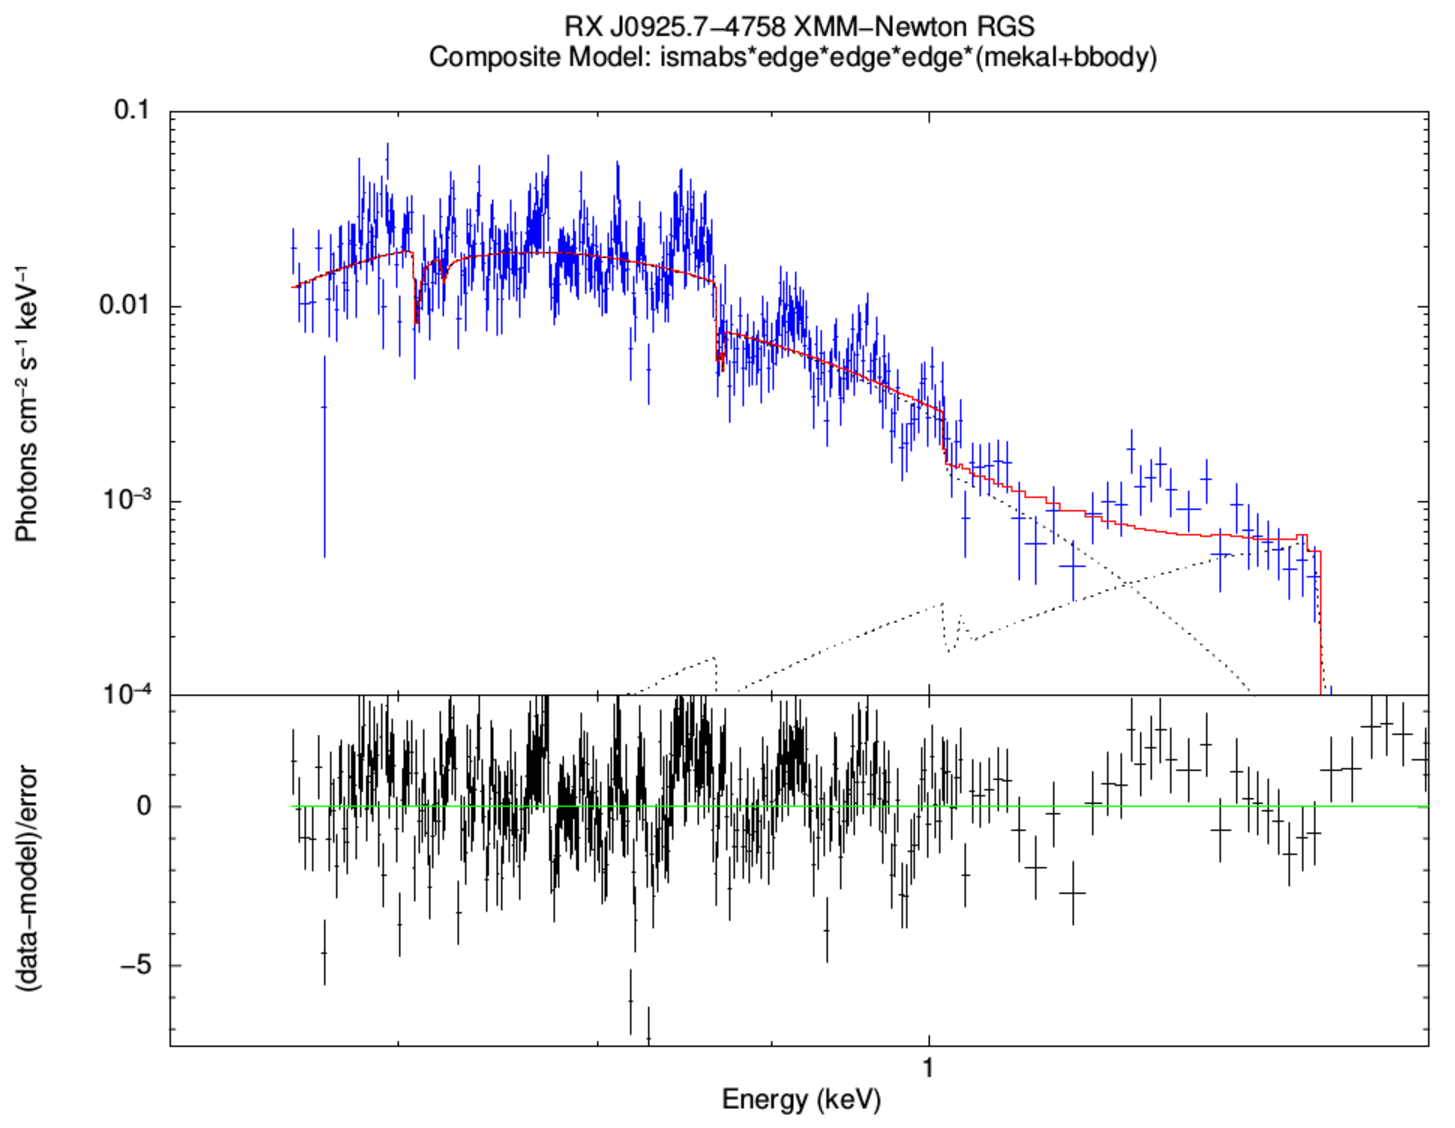
\includegraphics[scale=0.45]{mr-vel-xmm-rgs-03.pdf}}
%			\end{figure}
%			
%			This spectrum showed another improvement in the fit, which is reflected in the reduced $\chi^2$ value of 2.56. This fit shows the abundances for many species. NI, OI, NeI, MgI, SiI, ArI and Fe showing abundances of $1.06\times 10^{18}$, $4.61\times 10^{18}$, $1.67\times 10^{18}$, $3.61\times 10^{19}$, $5.54\times 10^{18}$, $5.20\times 10^{16}$ and $1.31\times 10^{17}$ respectively.
%			
%			However, the soft X-ray photons seen in the 1$^{\mathrm{st}}$ order spectrum seems to be missing in the  2$^{\mathrm{nd}}$ order spectrum. A fluxed spectrum comprising of data from both diffraction orders could be constructed and subsequently analysed.

	\setcounter{footnotecount}{\value{footnote}}